\documentclass[11pt]{article}

\usepackage[T1]{fontenc}
\usepackage{lmodern}
\usepackage[margin=1in]{geometry}
\usepackage{microtype}
\usepackage{amsmath}
\usepackage{amssymb}
\usepackage{array}
\usepackage{booktabs}
\usepackage{enumitem}
\usepackage{longtable}
\usepackage{tabularx}
\usepackage{graphicx}
\usepackage{float}
\usepackage{xcolor}
\usepackage{tikz}
\usetikzlibrary{arrows.meta,calc,fit,positioning,shapes.geometric,shapes.misc}
\usepackage{hyperref}

\hypersetup{
  colorlinks=true,
  linkcolor=black,
  citecolor=black,
  urlcolor=black,
  pdftitle={MPP-I: Machine Payments Protocol for Inference},
  pdfauthor={Alethieum; Jamie},
  pdfsubject={An MPP payment profile for inference execution, metering, and settlement},
  pdfkeywords={machine payments, metered inference payments, HTTP 402, MPP, x402, inference wallets, metered inference, streaming payments}
}

\setlength{\parindent}{0pt}
\setlength{\parskip}{0.65em}
\hyphenpenalty=10000
\exhyphenpenalty=10000
\emergencystretch=3em
\setlist[itemize]{topsep=0.25em,itemsep=0.15em,leftmargin=1.35em}
\setlist[enumerate]{topsep=0.25em,itemsep=0.15em,leftmargin=1.55em}
\renewcommand{\arraystretch}{1.15}
\newcommand{\field}[1]{\texttt{\detokenize{#1}}}
\newcommand{\mppi}{MPP-I}
\newcommand{\docversion}{Paper v1.0}
\newcommand{\publicationdate}{June 28, 2026}
\newcommand{\copyrightnotice}{Copyright (c) 2026 Alethieum. All rights reserved.}
\newcommand{\statusnotice}{Protocol proposal. Not legal, regulatory, tax, accounting, investment, or financial advice.}

\tikzset{
  actor/.style={draw, rounded corners=2pt, fill=white, minimum width=2.9cm, minimum height=0.82cm, align=center, font=\small},
  system/.style={draw, rounded corners=2pt, fill=gray!8, minimum width=3.0cm, minimum height=0.82cm, align=center, font=\small},
  rail/.style={draw, rounded corners=2pt, fill=gray!14, minimum width=3.0cm, minimum height=0.82cm, align=center, font=\small},
  process/.style={draw, rounded corners=2pt, fill=gray!6, minimum width=2.9cm, minimum height=0.82cm, align=center, font=\small},
  decision/.style={draw, diamond, aspect=2.15, fill=gray!12, align=center, inner sep=1.2pt, font=\scriptsize},
  state/.style={draw, rounded corners=2pt, fill=gray!8, minimum width=2.4cm, minimum height=0.76cm, align=center, font=\scriptsize},
  note/.style={draw, rounded corners=2pt, fill=white, align=left, font=\scriptsize, text width=3.4cm},
  flow/.style={-{Latex[length=2.2mm]}, thick},
  dataflow/.style={-{Latex[length=2.2mm]}, thick, black},
  payflow/.style={-{Latex[length=2.2mm]}, thick, black},
  riskflow/.style={-{Latex[length=2.2mm]}, thick, black, dashed}
}

\title{\textbf{\mppi{}: Machine Payments Protocol for Inference}\\\large Machine Payments for Metered Inference\\\normalsize An MPP payment profile for inference execution, metering, and settlement}
\author{Alethieum\\Written by Jamie\\Contact: \href{mailto:jamie@alethieum.com}{jamie@alethieum.com}}
\date{\docversion\\Publication date: \publicationdate}

\begin{document}

\maketitle

\begin{center}
{\small \copyrightnotice}\\[-0.15em]
{\small \statusnotice}
\end{center}

\begin{center}
\begin{minipage}{0.92\linewidth}
\small This paper is non-normative. In this paper, \emph{should} marks proposal-level guidance. Uses of \emph{must} identify safety invariants that a future formal profile should preserve, not final conformance language.
\end{minipage}
\end{center}

\begin{abstract}
\mppi{} (Machine Payments Protocol for Inference) is proposed as an MPP-native payment profile for metered inference. It is designed for autonomous agents, human users, applications, inference wallets, inference providers, settlement methods, facilitators, and blockchain networks that support machine payments. MPP and related Payment HTTP drafts supply the intended \field{402} challenge, credential, and receipt envelope. \mppi{} defines the inference-specific lifecycle inside that envelope.

\noindent Inference is not a fixed-price resource access call. A provider can publish machine-readable prices, bounds, and admission requirements, but the final delivered output length is not known when the request is admitted. The serving path must cover prompt tokenisation, prefill, scheduler admission, KV-cache allocation, autoregressive decode, output delivery, and final settlement. \mppi{} proposes run-scoped authorisation, cumulative credit grants, signed meter frames, low-credit and drain states, delivered-unit billing, settlement references, and final inference receipts. Its core design goal is to synchronise delivered-output production with payment authorisation, so agents, apps, users, wallets, and providers can use machine payments for metered inference without placing payment in the per-token critical path, while keeping authorisation ahead of the next disclosed admitted interval.
\end{abstract}

\textbf{Keywords:} machine payments, metered inference payments, HTTP 402, MPP, x402, inference wallets, metered inference, streaming payments.

\section*{Executive Summary}
\addcontentsline{toc}{section}{Executive Summary}

MPP-I is a proposed MPP-compatible, inference-native payment profile for metered inference.

MPP and related Payment HTTP efforts are defining a way for agents and apps to pay for API requests, tool calls, and content through an HTTP payment flow. That matters because agents that rely on external resources need a way to buy digital services without human checkout, account setup, invoices, or provider-specific commercial agreements for every call.

Inference is a central resource for that machine-payment flow. An agent may handle memory, tools, routing, policy, and workflow itself, but inference is what lets it reason, plan, generate, verify, and act. Agents that depend on external inference providers need a way to authorise bounded, metered inference when they need stronger reasoning, larger context, specialised capability, or higher reliability than they can run locally. Human users, apps, tools, and inference wallets can use the same payment flow to access inference providers through machine payments.

The problem is that inference does not behave like a fixed-price resource request. The final metered amount due is not known when prefill or scheduler admission begins. The provider must admit prefill, allocate scheduler and KV cache state, and run decode while output tokens are being produced. Once this begins, the provider is already spending scarce serving resources. Holding back the response does not remove that cost. Checking payment only after generation creates provider credit risk. Asking the buyer to authorise the worst case up front creates buyer over-authorisation.

Standard MPP sessions and x402 payment flows provide useful payment, voucher, cap, and settlement primitives, but they do not by themselves define the inference execution lifecycle. For inference, authorisation must remain ahead of admitted execution and be visible to the provider execution gate before the next metering boundary is admitted.

\mppi{} defines that lifecycle. It keeps MPP compatibility for the outer \field{402} challenge, credential, payment, and receipt flow, then adds semantics specific to inference: inference quotes, client policy, authorisation scoped to the run, cumulative vouchers or credit grants, signed meter frames, low-credit states, drain-entry behaviour, hard-stop boundary rules, settlement references, and final inference receipts.

The core execution gate has two related checks:

\[
\begin{aligned}
A_t^{\mathrm{gate}} &=
\min(A_t^{\mathrm{valid}},\mathrm{policy\_max\_total},\mathrm{run\_claimable\_limit}_t)\\
a_t \equiv \mathrm{available\_for\_new}_t &=
A_t^{\mathrm{gate}} - P_t - B_{\mathrm{active},t}\\
\mathrm{post\_admission\_finishable}_{j,t} &\iff
\forall i \in \mathcal{I}_t^{+j}:
a_{t,i}^{\mathrm{finish},+j} \geq H_{i,t}^{\mathrm{finish}(q)}\\
\mathrm{may\_admit\_new\_interval}_{j,t} &\iff
a_t \geq H_{j,t}^{\mathrm{admit}(q)}\\
&\quad\land\;
a_t \geq D_{j,t}\\
&\quad\land\;
\mathrm{ack\_lag\_ok}_t\\
&\quad\land\;
\mathrm{post\_admission\_finishable}_{j,t}\\
\mathrm{may\_finish\_interval}_{i,t} &\iff
a_{t,i}^{\mathrm{finish}} \geq H_{i,t}^{\mathrm{finish}(q)}\\
&\quad\land\;
\mathrm{ack\_lag\_ok}_t
\end{aligned}
\]

Here \(A_t\) is the latest accepted cumulative authorisation, \(A_t^{\mathrm{valid}}\) is the portion of that authorisation that is valid for the relevant gate decision under the grant-validity and settlement-method rules, and \(A_t^{\mathrm{gate}}\) is the portion currently usable by the execution gate after policy and run-claimability checks. \(P_t\) is boundary-posted cumulative amount due, \(B_{\mathrm{active},t}\) is the maximum cost bound of active admitted intervals not yet posted to due, \(C_i^{\max}\) is the admitted bound for interval \(i\), and \(a_{t,i}^{\mathrm{finish}}=A_t^{\mathrm{gate}}-P_t-(B_{\mathrm{active},t}-C_i^{\max})\). \(\mathcal{I}_t^{+j}\) is the active set that would exist after admitting candidate interval \(j\), and \(a_{t,i}^{\mathrm{finish},+j}\) is interval \(i\)'s hypothetical finish amount under that post-admission active set. Candidate interval \(j\) may be admitted only when its own admission headroom \(H_{j,t}^{\mathrm{admit}(q)}\), its drain-entry threshold \(D_{j,t}\), acknowledgement lag, and post-admission finishability all hold. The finish check only allows an already admitted bounded interval to reach its disclosed metering boundary while its own finish headroom remains covered. The acknowledgement-lag check keeps delivered but unacknowledged output within the profile's disclosed range, buffer, or exposure limit; it does not make unacknowledged output billable under the base profile.

The inference plane carries the private request and delivered output. The payment/control plane carries authorisation, vouchers, meter frames, low-credit events, drain events, settlement state, and receipts. These are logical planes, so they may be separate channels or multiplexed over a suitable transport.

If vouchers keep up, inference continues. If vouchers stop, the provider admits no new billable interval, uses only the already authorised headroom for the interval already admitted, stops at the disclosed boundary, settles the metered amount due, and emits a final receipt. Only output that satisfies the selected delivery and acknowledgement boundary is billable as output; under the base profile, delivered but unacknowledged output is reported separately or remains provider risk. Other units, such as prefill, cached input, tool calls, reasoning tokens, multimodal units, KV hold time, or accelerator time, are billable only if they are explicitly priced, metered, and receipted.

\mppi{} is therefore a specialised protocol within the MPP family. MPP makes machine payments possible for web resources. \mppi{} makes machine payments work for metered inference.

\begin{table}[htbp]
\centering
\caption{Paper thesis}
\label{tab:paper-thesis}
\begin{tabularx}{\linewidth}{>{\bfseries\raggedright\arraybackslash}p{0.22\linewidth} >{\raggedright\arraybackslash}X}
\toprule
Problem & Streaming inference has uncertain final metered amount due, provider-side prefill cost, scarce KV-cache state, and latency-sensitive token emission. \\
Today & Fixed charges, account balances, request-level caps, and standard payment sessions are useful patterns, but they do not standardise inference payment semantics. \\
Proposal & \mppi{} is proposed as a specialised profile within the MPP family. It defines quotes, policies, cumulative credit grants, meter frames, watermarks, drain and stop behaviour, settlement references, and final inference receipts for metered inference runs. \\
Protocol shape & MPP supplies the outer \field{402} challenge, credential, and receipt envelope. \mppi{} supplies the inference execution and metering lifecycle inside that envelope, including the payment/control path visible to the execution gate. \\
Outcome & Agents get bounded spend, providers get hard-bounded exposure under deterministic profiles or risk-budgeted exposure under disclosed quantile profiles, and wallets or facilitators can enforce policy without putting payment in the path of every token. \\
\bottomrule
\end{tabularx}
\end{table}

\textbf{Technical contribution.} \mppi{} specifies how an inference provider can bind request admission, prefill, decode continuation, cumulative metering, low-credit state, drain and stop behaviour, settlement, and final receipts to MPP-compatible payment authorisation.

\begin{figure}[H]
\centering
\resizebox{0.94\linewidth}{!}{%
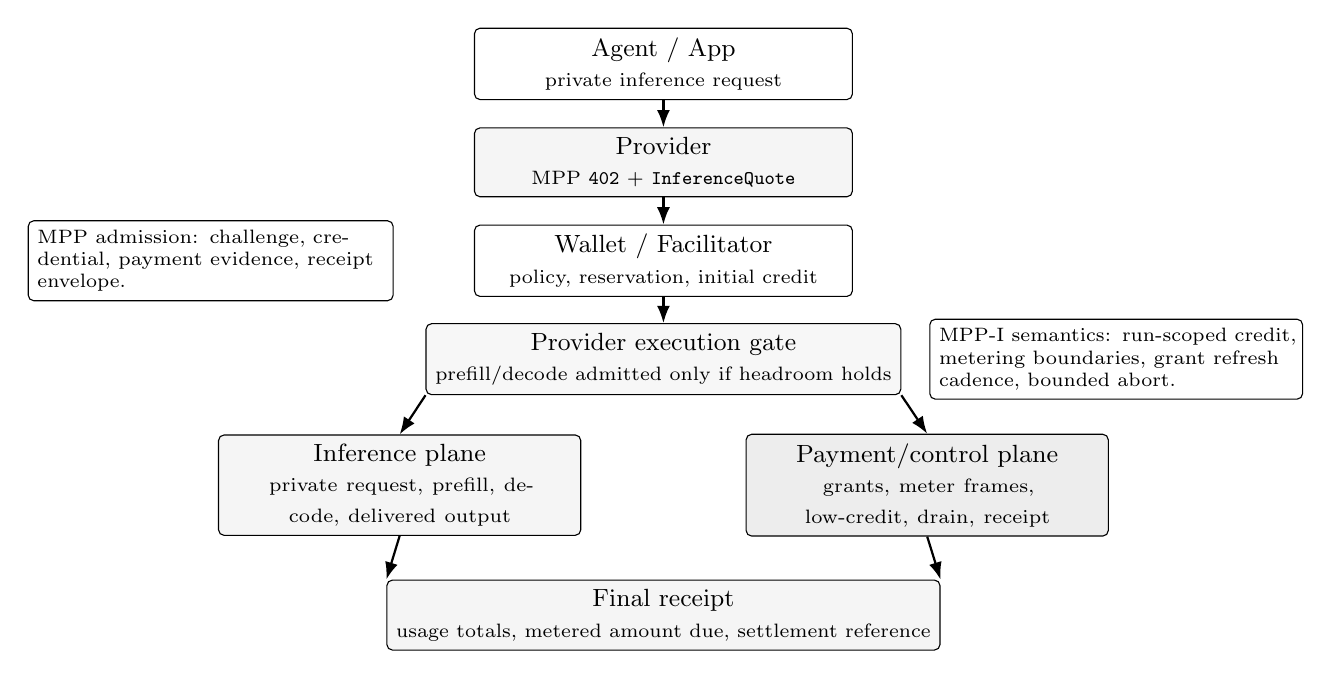
\begin{tikzpicture}[x=1cm,y=1cm]
  \node[actor, minimum width=4.8cm] (agent) at (0,0) {Agent / App\\\scriptsize private inference request};
  \node[system, minimum width=4.8cm] (challenge) at (0,-1.25) {Provider\\\scriptsize MPP \field{402} + \field{InferenceQuote}};
  \node[actor, minimum width=4.8cm] (wallet) at (0,-2.5) {Wallet / Facilitator\\\scriptsize policy, reservation, initial credit};
  \node[process, minimum width=4.8cm] (gate) at (0,-3.75) {Provider execution gate\\\scriptsize prefill/decode admitted only if headroom holds};

  \node[system, minimum width=4.6cm, text width=4.15cm] (inference) at (-3.35,-5.35)
    {Inference plane\\\scriptsize private request, prefill, decode, delivered output};
  \node[rail, minimum width=4.6cm, text width=4.15cm] (control) at (3.35,-5.35)
    {Payment/control plane\\\scriptsize grants, meter frames, low-credit, drain, receipt};
  \node[system, minimum width=4.8cm] (receipt) at (0,-7.0) {Final receipt\\\scriptsize usage totals, metered amount due, settlement reference};

  \draw[flow] (agent.south) -- (challenge.north);
  \draw[flow] (challenge.south) -- (wallet.north);
  \draw[flow] (wallet.south) -- (gate.north);
  \draw[dataflow] (gate.south west) -- (inference.north);
  \draw[payflow] (gate.south east) -- (control.north);
  \draw[dataflow] (inference.south) -- (receipt.north west);
  \draw[payflow] (control.south) -- (receipt.north east);

  \node[note, text width=4.4cm] at (-5.75,-2.5)
    {MPP admission: challenge, credential, payment evidence, receipt envelope.};
  \node[note, text width=4.5cm] at (5.75,-3.75)
    {\mppi{} semantics: run-scoped credit, metering boundaries, grant refresh cadence, bounded abort.};
\end{tikzpicture}%
}
\caption{\mppi{} at a glance. MPP provides interoperable payment admission; \mppi{} defines the inference execution and metering lifecycle after admission.}
\label{fig:mppi-at-a-glance}
\end{figure}

\tableofcontents
\newpage

\section{Introduction}

Machine payment protocols are turning HTTP payment into a usable web primitive: a machine client can request a resource, receive a payment challenge, satisfy it, and get a receipt. That pattern works well for fixed price API calls, paywalled content, file downloads, and other resources whose price is known before delivery.

Metered inference has a different shape. A provider is doing more than releasing a known object after payment. It is admitting a stateful online inference-serving request whose final metered amount due is only partly known when prefill or scheduler admission begins. The prompt must be tokenised and priced. The prefill phase runs before the first visible output token. The request may hold scheduler capacity and key-value cache state. The output length is unknown until generation stops. If payment authorisation stops during a run, the provider can only continue through already authorised headroom before stopping at a disclosed enforcement boundary.

This is the gap \mppi{} targets. MPP and related Payment HTTP drafts are defining a common way for machine clients to request payment, satisfy a payment challenge, and receive receipts \cite{mpp}. \mppi{} keeps the MPP outer flow and adds the payment lifecycle needed once the paid resource is an inference run:

\begin{quote}
\small\raggedright\textbf{\mppi{} gives metered inference an MPP-native payment profile: inference delivery and payment control are separate logical planes, carried on separate channels or multiplexed with independent control flow, while cumulative authorisation remains ahead of admitted inference execution.}
\end{quote}

The core rule is a two-gate admission model. In the formulas below, \(a_t=A_t^{\mathrm{gate}}-P_t-B_{\mathrm{active},t}\), where \(A_t^{\mathrm{gate}}\) is the latest accepted cumulative authorisation after grant-validity, policy, and run-claimability clamping, \(P_t\) is boundary-posted cumulative amount due, and \(B_{\mathrm{active},t}\) is the active admitted bound. For an already admitted interval \(i\), \(a_{t,i}^{\mathrm{finish}}=A_t^{\mathrm{gate}}-P_t-(B_{\mathrm{active},t}-C_i^{\max})\). For candidate interval \(j\), post-admission finishability means:

\[
\mathrm{post\_admission\_finishable}_{j,t}
\iff
\forall i \in \mathcal{I}_t^{+j}:
a_{t,i}^{\mathrm{finish},+j} \geq H_{i,t}^{\mathrm{finish}(q)}
\]

where \(\mathcal{I}_t^{+j}\) is the active set after hypothetically adding \(j\), and \(a_{t,i}^{\mathrm{finish},+j}\) is interval \(i\)'s hypothetical finish amount under that set.

\[
\begin{aligned}
\mathrm{may\_admit\_new\_interval}_{j,t} \iff
{}&a_t \geq H_{j,t}^{\mathrm{admit}(q)}\\
&\land a_t \geq D_{j,t}\\
&\land \mathrm{ack\_lag\_ok}_t\\
&\land \mathrm{post\_admission\_finishable}_{j,t}
\end{aligned}
\]

\[
\begin{aligned}
\mathrm{may\_finish\_interval}_{i,t} \iff
{}&a_{t,i}^{\mathrm{finish}} \geq H_{i,t}^{\mathrm{finish}(q)}\\
&\land \mathrm{ack\_lag\_ok}_t
\end{aligned}
\]

New billable intervals may be admitted only while the available amount for new work covers the candidate interval's admission headroom \(H_{j,t}^{\mathrm{admit}(q)}\), the candidate drain-entry threshold \(D_{j,t}\), the acknowledgement-lag guard, and the finishability of all intervals that would be active after admission. An already admitted bounded interval \(i\) may finish only while its interval-specific finish amount remains at or above the required finish headroom \(H_{i,t}^{\mathrm{finish}(q)}\). When \(H_{i,t}^{\mathrm{finish}(q)} \leq a_{t,i}^{\mathrm{finish}}\) but the next candidate admission guard fails, the run is draining: admitted intervals may reach their disclosed boundaries, but the provider must not admit another billable interval until credit is restored. The formal section defines these values from boundary-posted amount due and active admitted bounds. In the base paper profile, delivered but unacknowledged output is provider risk and does not advance \field{cumulative_amount_due}. The buyer does not need to authorise a large worst case payment up front. The provider does not need to continue inference beyond claimable payment state or the acknowledgement boundary. The payment system does not need to sit in the critical path for every token.

\textbf{Illustrative example.} An agent asks a provider for streamed inference. The provider replies with an \mppi{} quote containing the inference target, tokenizer version, serialisation profile, prefill/input price, delivered-output price, accepted billable units, required initial credit, low and drain-entry watermarks, and metering-boundary policy. The wallet authorises only that run. Meter frames report cumulative delivered usage; grant refreshes are accepted before the next per-run admitted interval. If grants stop, the provider drains through already authorised headroom and stops at the disclosed boundary.

Assume an illustrative tariff of \$200 per million billable units, with the same unit price used for input/prefill tokens and delivered output tokens. Each billable unit costs \$0.0002. A request with 60{,}000 input tokens and an initial 10{,}000 delivered-output-token headroom therefore needs \$14 of initial authorisation. If the delivered output reaches 42{,}000 tokens, the cumulative metered amount due is \$20.40 before any separately quoted units such as cached input, tool calls, reasoning tokens, multimodal units, KV-cache hold intervals, or scheduler-admitted accelerator intervals. The final receipt reports actual metered usage, \field{settlement_cap}, \field{settlement_target_amount}, \field{run_claimable_limit}, \field{settled_amount}, unused authorisation, released run claimable amount or reservation, and refund amount if applicable. The numbers are illustrative, not normative.

This paper contributes product and protocol framing, not a final standard or registered protocol number. It argues that \mppi{} should be specified as an MPP payment profile for inference, using \field{inference} as the proposed payment intent name. Until \field{inference} is registered or otherwise accepted by the relevant MPP or Payment HTTP process, experimental deployments should identify it as a private or provisional \mppi{} profile identifier, or carry it under a registered intent through a profile-specific adapter, and bind that profile identifier to the challenge, quote, policy, grants, meter frames, and final receipt. In this paper, \emph{intent} means the payment purpose advertised through the MPP payment challenge. \emph{Profile} means the \mppi{} lifecycle rules, object fields, transport expectations, and settlement semantics that make that intent workable for metered inference.

\section{Audience and Scope}

This paper is written for inference providers, agent builders, app teams, inference wallet teams, payment facilitators, settlement-method builders, blockchain networks, protocol engineers, and decentralised inference networks. It assumes the reader understands HTTP APIs, tokenisation, prefill/decode accounting, and usage-based inference pricing, but it does not assume deep payment channel or inference engineering expertise.

The scope is focused. \mppi{} is a payment profile for metered inference. It can produce signed records of inference target, tokenizer ID, usage, timing, content-private commitments, metered amount due, and settlement reference. It does not prove inference quality. It does not solve legal compliance, consumer disputes, chargebacks, tax, sanctions screening, or all settlement finality questions. Those systems can be implemented around \mppi{}, but the profile should not claim to provide them.

This paper is not legal, regulatory, tax, accounting, investment, or financial advice. It does not recommend any payment method, asset, facilitator, wallet, jurisdiction, or compliance posture. Terms such as wallet, facilitator, settlement, reservation, and claimability are used as protocol design roles and state descriptions, not as determinations of legal status. Implementers remain responsible for evaluating licensing, money transmission, anti-money-laundering obligations, sanctions, consumer protection, tax, data protection, and settlement finality obligations for their jurisdictions, counterparties, and selected payment methods.

\section{Background: Machine Payments and MPP Compatibility}

Current machine payment work is converging around HTTP 402, signed payment authorisations, stablecoin settlement, facilitators, payment sessions, and off-chain vouchers. These draft and implementation primitives are useful, and \mppi{} should reuse them where the selected profile supports the same semantics. The problem is that they mostly answer payment admission and settlement questions. \mppi{} addresses the inference execution lifecycle questions involved in admitting, continuing, draining, stopping, settling, and receipting an inference run.

As of June 28, 2026, Payment HTTP authentication and related MPP materials are active draft work. This paper therefore uses MPP compatibility as an interoperability target, not as a claim that \mppi{} is already standardised. Mutable documentation references were checked on June 28, 2026; a final standards-track release should prefer dated drafts, release versions, permalinks, or archived snapshots where available.

\subsection{Payment HTTP Authentication}

The relevant primitive is the emerging \field{Payment} HTTP authentication scheme. A server can return \field{402 Payment Required} with a \field{WWW-Authenticate: Payment} challenge; the client fulfils the payment requirement and retries with an \field{Authorization: Payment} credential; the server verifies or settles the payment and returns the protected resource with an optional \field{Payment-Receipt} \cite{paymentauth}.

The key design choice is extensibility. The \field{Payment} scheme is payment method agnostic. Concrete payment methods define their own request schemas, payload schemas, verification rules, and settlement procedures. Payment intents describe the type of payment being requested, and intent specifications define semantic meaning, request fields, payload requirements, verification, and settlement semantics \cite{paymentauth}.

Payment HTTP authentication is a good envelope for \mppi{}. \mppi{} can be defined around a proposed \field{inference} payment intent rather than as a new HTTP payment framework. Before any formal registration, a deployed profile should treat \field{inference} as a private or provisional profile identifier, or carry it through a registered intent with a profile-specific adapter, so early experiments do not imply standards-track wire compatibility. The missing layer is inference execution semantics: the \field{Payment} scheme does not say how much inference may be executed after a partial authorisation, when low-credit warnings should fire, when a provider must drain and stop, or what an inference receipt must contain.

Large inference quotes and receipts should not be forced into oversized payment headers. The \mppi{} profile should allow compact header payloads containing IDs, hashes, short fields for the selected method, and references to signed quote or receipt bodies. Any referenced object must be bound by digest to the challenge or credential so it cannot be swapped after approval.

The \mppi{} \field{FinalReceipt} is not automatically the same object as the HTTP \field{Payment-Receipt} header. A profile may carry or reference a \field{FinalReceipt} through \field{Payment-Receipt} only where the underlying HTTP response semantics allow it. Otherwise, \field{FinalReceipt} should be treated as a signed control plane object, response body, trailer, or referenced receipt object that is bound back to the payment challenge, run, policy, meter frames, and settlement reference.

\subsection{Charge-Style Payments and Stablecoins}

The \field{charge} intent for Payment HTTP authentication defines a one-time exchange of payment for resource access \cite{chargeintent}. The payer provides proof of payment, or a signed authorisation to collect payment, and the server grants access. Method-specific drafts define how this works over particular settlement methods, such as EVM ERC-20 transfers or Solana SPL tokens \cite{evmcharge,solanacharge}. Stablecoin-denominated charge methods can be useful in the same family because they standardise fixed machine payments over supported settlement paths.

Charge-style payments are useful for fixed API calls, quote fees, cached results, deposits, initial prefill grants, and final settlement. They are not enough for open-ended streaming inference. A fixed charge assumes the amount is known before access is granted. A generation may end after 20 output tokens or 2{,}000. The fixed charge primitive can carry money, but it does not decide how inference proceeds while cost is still accumulating.

\subsection{x402}

x402 uses HTTP 402 to let clients pay for web resources programmatically. Its \field{exact} scheme is fixed price: the seller advertises one amount, the buyer signs that amount, and a facilitator settles the payment for the request \cite{x402exact}. This works when the final charge is known before the response is generated.

x402's \field{upto} scheme is a useful adjacent payment primitive. The buyer authorises a maximum for one request, and the seller settles actual usage up to that maximum. The x402 documentation explicitly names LLM token generation, bandwidth, compute time, and dynamic data queries as use cases \cite{x402upto}. This can settle unknown actual usage under a request-level cap, but it is still not an inference execution-control protocol. During streamed generation, the primary response path is occupied by inference output. If the provider only computes or settles actual usage after the response completes, it has not observed fresh claimable authorisation while prefill and decode were consuming serving capacity. A high cap protects the provider and over-authorises the buyer. A low cap protects the buyer and risks truncation at the wrong boundary.

x402's \field{batch-settlement} scheme addresses another practical issue: high-throughput settlement. It uses escrow, off-chain cumulative vouchers, fast server verification, and later batched on-chain redemption \cite{x402batch}. That mechanism is useful for repeated inference calls and small meter increments. It is still a settlement mechanism unless its vouchers are run-bound, forward-looking, sequenced, and visible to the inference execution gate before the next boundary is admitted. \mppi{} must define the run lifecycle, buffer policy, meter cadence, low-credit and drain behaviour, stop behaviour, and receipt fields. x402-compatible caps, facilitators, or batch-settlement paths are compatible with \mppi{} only when paired with an inference payment/control path that carries run-bound cumulative grants, meter acknowledgements, low-credit signals, and stop or drain state before the next metering boundary is admitted.

The compatibility point needs precision. Payment HTTP authentication uses \field{WWW-Authenticate: Payment}, \field{Authorization: Payment}, and \field{Payment-Receipt} headers. x402 uses HTTP 402 concepts and payment flows backed by facilitators, but its wire objects and headers are not automatically the same as Payment HTTP authentication. \mppi{} can use settlement paths or adapters compatible with x402 where they preserve run binding, cumulative authorisation, and receipt semantics, but that is compatibility by profile and adapter, not automatic wire equivalence.

\subsection{MPP Sessions}

MPP session patterns are the closest existing primitive. A session intent establishes reusable funding or voucher state for metered usage, often using escrow and off-chain vouchers so the client can authorise increasing cumulative amounts without settling a separate payment for every streamed chunk. Current MPP session materials explicitly discuss high-frequency, pay-as-you-go usage: a client funds reusable payment state, the server delivers metered work, the client authorises cumulative amounts, and the server settles periodically or at stream completion \cite{mppsession}.

MPP sessions are a useful adoption bridge for \mppi{}, but the distinction matters. A standard payment session says how value is incrementally authorised. It becomes an \mppi{} deployment only when session updates are coupled to the provider's prefill and decode gates during the run. \mppi{} adds that coupling: prefill starts only after initial run-bound credit; decode continues only while the latest accepted voucher or credit grant covers the next disclosed metering boundary; low-credit, drain, stop, and receipt messages are sequenced against delivered output and metered usage. Semantics for inference should not be hidden inside provider-specific policy.

\subsection{Related Work and Prior-Art Positioning}

Adjacent agent-payment work is complementary rather than equivalent. Google's Agent Payments Protocol (AP2) focuses on agent-led payment authority, accountability, and commerce across payment methods, while the A2A x402 extension brings on-chain x402 payments into agent-to-agent service flows \cite{ap2,a2ax402}. These efforts help explain why agents need interoperable payment authority, but they do not define an inference provider's prefill, decode, low-credit, drain, stop, and final receipt lifecycle.

There is also direct adjacent work on usage-based inference settlement. Polygon's x402 per-inference guide uses the \field{upto} scheme so a buyer authorises a per-call maximum and the server settles actual token, compute, or output usage after measuring it \cite{polygonInferenceBilling}. Fortytwo's x402Escrow extends x402 with escrow for usage-based, pay-per-token AI services where cost is unknown at request time \cite{fortytwoEscrow}. These are important prior-art signals: they show the market is already moving toward accountless, usage-based inference payment. As published, they primarily address capped settlement, middleware, or escrow mechanics. \mppi{} addresses the inference execution boundary itself: it specifies run-scoped authorisation, scheduler-visible payment state, admitted intervals, cumulative grants, meter frames, delivery acknowledgements, low-credit and drain semantics, stop boundaries, and final inference receipts.

Security work on x402 also supports making these bindings explicit. A 2026 analysis of x402-enabled payment systems identifies state-synchronisation and logic-flaw classes such as cross-resource substitution, duplicate-settlement race conditions, allowance overdraft, and denial of settlement in agentic payment flows \cite{x402LogicFlaws}. \mppi{} treats those risks as protocol-design requirements: run identifiers, request commitments, claim references, cumulative monotonic grants, meter-frame sequencing, delivery acknowledgements, and idempotent final receipts are not implementation decoration; they are the control surface that keeps payment state tied to the inference work being admitted.

\begin{table}[H]
\centering
\caption{Existing protocols and the inference execution-control gap}
\label{tab:existing-protocols-gap}
\begin{tabularx}{\linewidth}{>{\raggedright\arraybackslash}p{0.18\linewidth} >{\raggedright\arraybackslash}X >{\raggedright\arraybackslash}X}
\toprule
\textbf{Protocol} & \textbf{What it solves} & \textbf{Gap for inference} \\
\midrule
Payment HTTP authentication & HTTP 402 challenge, credential, receipt, method and intent negotiation. & No inference execution lifecycle, execution-visible payment state, low-credit, or delivered unit billing semantics. \\
x402 \field{exact} & Fixed price payment when final amount is known before response. & Final inference cost is often unknown at admission. \\
x402 \field{upto} & Maximum authorisation for one request with actual usage settlement. & Does not define rolling top-ups, low-credit states, or decode continuity. \\
x402 batch settlement & Escrow and cumulative vouchers for high throughput settlement. & Settlement substrate unless vouchers are run-bound, forward-looking, sequenced, and visible to the execution gate before the next boundary. \\
MPP Session & Funding or voucher substrate using escrow, off-chain vouchers, or equivalent cumulative authorisation. & Session substrate; lacks prefill, decode, drain/stop, content-private metering, and final receipt rules for inference. \\
Stablecoin charge & Fixed denomination charge or settlement method. & Useful for deposits and settlement, but not dynamic execution control. \\
\bottomrule
\end{tabularx}
\end{table}


\section{Current State Payment Flows}

Most machine payment protocols today are optimised for resource access and payment admission, not execution control inside an online inference-serving path. They can challenge a client, verify a payment credential, settle a fixed or capped amount, and return a resource. That is enough when the price is known before delivery. It is incomplete when the resource is an inference run whose cost evolves during prefill, decode, tool use, and possible state hold.

\subsection{Fixed Price HTTP 402 Pattern}

Figure~\ref{fig:today-fixed-402} shows the common fixed price pattern. The key property is that the seller can state the amount before granting access. That maps cleanly to content, file downloads, cached API results, and bounded fixed price calls. It does not say what should happen while decode is still producing output and the final metered amount due is unknown.

\begin{figure}[H]
\centering
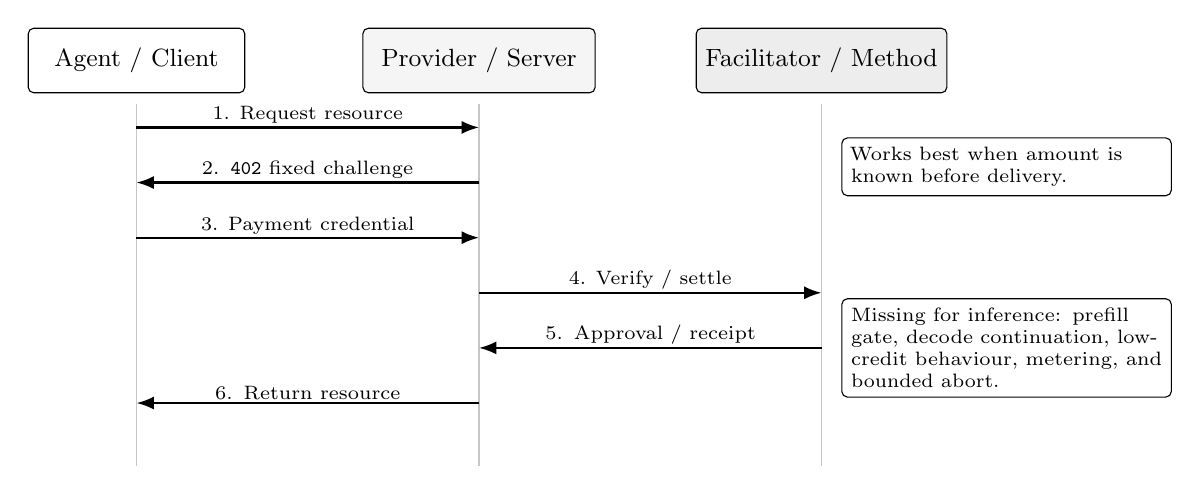
\begin{tikzpicture}[x=1cm,y=1cm]
  \node[actor, minimum width=2.75cm] at (0,0) {Agent / Client};
  \node[system, minimum width=2.95cm] at (4.35,0) {Provider / Server};
  \node[rail, minimum width=2.95cm] at (8.7,0) {Facilitator / Method};

  \foreach \x in {0,4.35,8.7} {\draw[gray!45] (\x,-0.55) -- (\x,-5.15);}

  \draw[flow] (0,-0.85) -- node[above,align=center,font=\scriptsize,fill=white,inner sep=1pt]{1. Request resource} (4.35,-0.85);
  \draw[flow] (4.35,-1.55) -- node[above,align=center,font=\scriptsize,fill=white,inner sep=1pt,text width=3.45cm]{2. \field{402} fixed challenge} (0,-1.55);
  \draw[payflow] (0,-2.25) -- node[above,align=center,font=\scriptsize,fill=white,inner sep=1pt]{3. Payment credential} (4.35,-2.25);
  \draw[payflow] (4.35,-2.95) -- node[above,align=center,font=\scriptsize,fill=white,inner sep=1pt]{4. Verify / settle} (8.7,-2.95);
  \draw[payflow] (8.7,-3.65) -- node[above,align=center,font=\scriptsize,fill=white,inner sep=1pt,text width=3.25cm]{5. Approval / receipt} (4.35,-3.65);
  \draw[dataflow] (4.35,-4.35) -- node[above,align=center,font=\scriptsize,fill=white,inner sep=1pt,text width=3.1cm]{6. Return resource} (0,-4.35);

  \node[note, text width=3.95cm] at (11.05,-1.35) {Works best when amount is known before delivery.};
  \node[note, text width=3.95cm] at (11.05,-3.65) {Missing for inference: prefill gate, decode continuation, low-credit behaviour, metering, and bounded abort.};
\end{tikzpicture}
\caption{Today: fixed price HTTP 402 resource access flow.}
\label{fig:today-fixed-402}
\end{figure}

\subsection{Single-Channel Streaming Payment Failure}

In a conventional streamed inference API, the primary response path carries output events such as SSE chunks, WebSocket messages, or gRPC stream messages. If payment checks rely on that same occupied response path, the provider has two poor choices. It can interrupt output while waiting for fresh payment state, which damages time to first token or inter-token latency. Or it can continue prefill and decode, then check payment after generation, which does not bound maximum unpaid admitted work because the serving cost has already been incurred. The failure is not value transfer in isolation; it is the absence of a run-scoped payment/control path that keeps claimable authorisation ahead of prefill and decode and is visible to the execution gate before the next metering boundary.

Request-level caps reduce the problem but do not solve inference metering. A large cap over-authorises the buyer. A small cap truncates the run or forces a stop at a boundary that may not match the serving engine's safe metering point. A generic session or voucher stream helps only if its updates are visible to the execution gate before the next prefill/decode interval is admitted.

\begin{figure}[H]
\centering
\resizebox{\linewidth}{!}{%
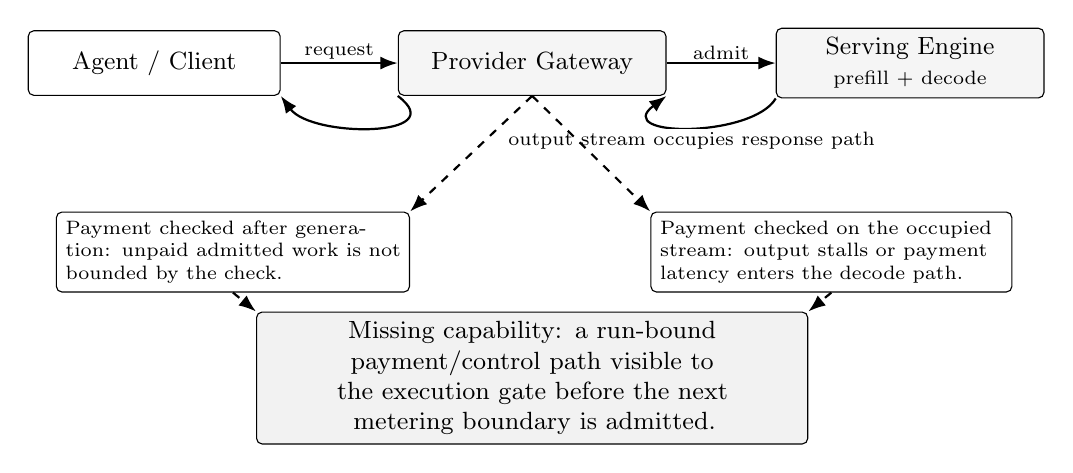
\begin{tikzpicture}[x=1cm,y=1cm]
  \node[actor, minimum width=3.2cm] (client1) at (-4.8,0) {Agent / Client};
  \node[system, minimum width=3.4cm] (provider1) at (0,0) {Provider Gateway};
  \node[system, minimum width=3.4cm] (sched1) at (4.8,0) {Serving Engine\\\scriptsize prefill + decode};

  \draw[dataflow] (client1.east) -- node[above,font=\scriptsize,fill=white,inner sep=1pt]{request} (provider1.west);
  \draw[dataflow] (provider1.east) -- node[above,font=\scriptsize,fill=white,inner sep=1pt]{admit} (sched1.west);
  \draw[dataflow] (sched1.south west) .. controls (2.8,-0.95) and (1.0,-0.95) .. node[below,font=\scriptsize,fill=white,inner sep=1pt]{output stream occupies response path} (provider1.south east);
  \draw[dataflow] (provider1.south west) .. controls (-1.0,-0.95) and (-2.8,-0.95) .. (client1.south east);

  \node[note, text width=4.25cm] (late) at (-3.8,-2.4)
    {Payment checked after generation: unpaid admitted work is not bounded by the check.};
  \node[note, text width=4.35cm] (stall) at (3.8,-2.4)
    {Payment checked on the occupied stream: output stalls or payment latency enters the decode path.};

  \node[process, text width=6.6cm, minimum width=7.0cm, fill=gray!10] (gap) at (0,-4.0)
    {Missing capability: a run-bound payment/control path visible to the execution gate before the next metering boundary is admitted.};

  \draw[riskflow] (provider1.south) -- (late.north east);
  \draw[riskflow] (provider1.south) -- (stall.north west);
  \draw[riskflow] (late.south) -- (gap.north west);
  \draw[riskflow] (stall.south) -- (gap.north east);
\end{tikzpicture}%
}
\caption{Single-channel streaming failure. The inference output stream does not provide an execution-visible payment/control path that can safely gate the next metering boundary.}
\label{fig:today-inference-options}
\end{figure}

The missing piece is not another provider-specific billing system. It is a shared inference payment state machine that agents, apps, inference wallets, and inference providers can all evaluate. Without that state machine, every provider has to define its own meanings for \field{low_credit}, \field{draining}, \field{stopped}, grant refresh timing, settlement, and final receipts.

\section{Why Inference Is Different}

Inference is economically closer to a metered, stateful compute session than to a fixed price content retrieval. The cumulative metered amount due can be bounded by policy, but exact usage is not known at request admission.

\subsection{Prefill, Decode, and Latency}

Modern text-generation serving usually separates inference into two phases. Prefill processes the input prompt and prepares the state needed for generation. Decode generates output tokens autoregressively, one step at a time. NVIDIA's benchmarking documentation defines time to first token (TTFT) as the time from request submission to the first output token and notes that TTFT generally includes queuing, prefill, and network latency \cite{nvidiaMetrics}. It defines inter-token latency as the latency between consecutive output tokens, a measure tied to the decode portion of a request \cite{nvidiaMetrics}.

This phase structure matters for payment. The provider incurs meaningful cost before the buyer sees the first useful output. The provider cannot know the final output length at the moment it accepts the request. Even when a buyer supplies \field{max_tokens}, that value is an upper bound, not the final metered amount due.

Production systems expose this uncertainty in their own quota systems. Amazon Bedrock illustrates the same reservation versus actual usage distinction in quota form: it reserves quota up front using input-related tokens and the requested output bound, adjusts quota during or after processing according to actual output and provider-specific burndown behaviour, and bills for actual token usage \cite{bedrockQuota}. That pattern is not a payment protocol, but it illustrates the same structural problem: admission wants a reservation, while settlement wants actual usage.

For \mppi{}, admission should make prefill cost explicit before serving-engine execution. A provider can tokenise and price the request before issuing an executable quote, or it can issue a conservative prefill bound and correct the quote before prefill begins. In either case, the initial credit grant should cover exact or conservatively bounded prefill cost plus the first execution headroom:

\[
\mathrm{required\_initial\_credit} =
\left\lceil
C_{\mathrm{prefill},0}^{\mathrm{bound}} + H_{\mathrm{decode},0}^{\mathrm{admit}(q)}
\right\rceil_{\mathrm{unit}}
\]

Here \(\lceil x\rceil_{\mathrm{unit}}\) means rounding up to the smallest unit of the selected payment or settlement method after applying the quoted price schedule.

Here \(C_{\mathrm{prefill},0}^{\mathrm{bound}}\) is the exact or conservative money-denominated prefill cost disclosed in the quote, and \(H_{\mathrm{decode},0}^{\mathrm{admit}(q)}\) is the admission headroom for the first decode interval under the selected profile. This one-step initial-credit formula applies only when the quoted prefill cost is exact or conservatively bounded through the next enforceable prefill boundary. Chunked or long-running prefill profiles must define \(C_{\mathrm{next},t}^{\max}\), \(H_{j,t}^{\mathrm{admit}(q)}\), metering cadence, and stop behaviour for prefill segments before decode admission. A profile may use a two-gate procedure instead: admit prefill under the prefill bound, meter it, then admit decode only after the payer has authorised the first decode headroom.

An executable quote needs to bind more than a model name and a tokenizer name. It should bind the serialisation and tokenisation surface that determines input length and prefill cost: tokenizer ID and version, chat template or canonical serialisation profile, special-token policy, tool or function schema hash, multimodal preprocessing profile where used, context-window and truncation policy, cache-hit class, and the exact or conservative input-token count. The payment/control plane should bind these fields by ID, digest, or hiding commitment. It should not receive the raw prompt or raw serialised request.

\begin{figure}[H]
\centering
\resizebox{\linewidth}{!}{%
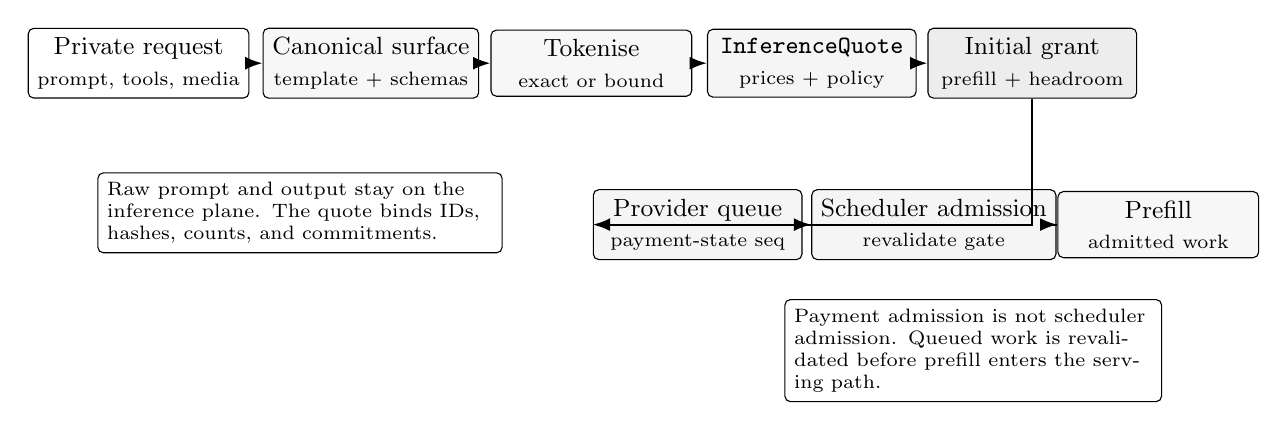
\begin{tikzpicture}[x=1cm,y=1cm]
  \node[actor, minimum width=2.65cm] (req) at (-6.0,0) {Private request\\\scriptsize prompt, tools, media};
  \node[process, minimum width=2.7cm] (canon) at (-3.05,0) {Canonical surface\\\scriptsize template + schemas};
  \node[process, minimum width=2.55cm] (tok) at (-0.25,0) {Tokenise\\\scriptsize exact or bound};
  \node[system, minimum width=2.65cm] (quote) at (2.55,0) {\field{InferenceQuote}\\\scriptsize prices + policy};
  \node[rail, minimum width=2.65cm] (grant) at (5.35,0) {Initial grant\\\scriptsize prefill + headroom};

  \node[system, minimum width=2.65cm] (queue) at (1.1,-2.05) {Provider queue\\\scriptsize payment-state seq};
  \node[system, minimum width=2.9cm] (sched) at (4.1,-2.05) {Scheduler admission\\\scriptsize revalidate gate};
  \node[process, minimum width=2.55cm] (prefill) at (6.95,-2.05) {Prefill\\\scriptsize admitted work};

  \draw[dataflow] (req.east) -- (canon.west);
  \draw[dataflow] (canon.east) -- (tok.west);
  \draw[flow] (tok.east) -- (quote.west);
  \draw[payflow] (quote.east) -- (grant.west);
  \draw[payflow] (grant.south) |- (queue.west);
  \draw[flow] (queue.east) -- (sched.west);
  \draw[flow] (sched.east) -- (prefill.west);

  \node[note, text width=4.9cm] at (-3.95,-1.9)
    {Raw prompt and output stay on the inference plane. The quote binds IDs, hashes, counts, and commitments.};
  \node[note, text width=4.55cm] at (4.6,-3.65)
    {Payment admission is not scheduler admission. Queued work is revalidated before prefill enters the serving path.};
\end{tikzpicture}%
}
\caption{Executable quote and prefill admission path. \mppi{} binds the serialisation and tokenisation surface, then requires claimable initial credit before queued work becomes scheduler-admitted inference work.}
\label{fig:executable-quote-admission}
\end{figure}

\subsection{KV Cache and Scheduler State}

KV cache is not accounting trivia. It is a scarce serving resource. The PagedAttention paper argues that high-throughput inference serving is constrained by key-value cache memory that is large and dynamically changes as requests grow and shrink \cite{pagedAttention}. vLLM's public write-up explains the same issue in operational terms: KV cache can be large, depends on sequence length, and inefficient management wastes memory through fragmentation and over-reservation \cite{vllmBlog}.

This is why the word ``pause'' should be used carefully. A provider can stop sending bytes to a client, but the request is either retained in scheduler state with KV-cache state resident, or it is evicted and must be recomputed or restarted. The cost is implementation-dependent and load-dependent, but it is not zero in systems optimised for low latency and high utilisation.

If a profile makes KV hold time billable, it should define the meter rather than naming the resource loosely. Useful fields include run or cache scope, token span, residency tier, start and end time, maximum hold, eviction policy, recompute behaviour, and whether the meter is provider-asserted, audited, or attested. Active-request KV, reusable prefix cache, offloaded KV, and evicted state have different costs and different verification properties.

In disaggregated serving, prefill, KV transfer, and decode may run on different workers or queues. \mppi{} does not need a separate protocol for that shape. The profile should treat each exposed phase as a distinct admitted interval when it is billable: prefill admission, KV transfer or residency, and decode continuation each need an explicit quote, meter, receipt field, and headroom boundary.

Payment headroom is not the only admission policy. A production profile should also let providers disclose queue timeout, priority class, per-wallet or per-tenant concurrency, active KV-token cap, overload rejection behaviour, reservation expiry, and reservation release rules. These fields should describe the provider's admission policy; \mppi{} should not try to impose a single universal scheduler fairness algorithm.

\subsection{Streaming Tightens the Tradeoff}

Streaming is a product feature, not just a transport detail. A metered inference protocol has to preserve low TTFT, stable output-token cadence, and bounded inter-token latency under typical conditions. If every token waits for an on-chain transfer or a human wallet approval, the serving path fails. If the provider streams a long answer before payment state is claimable, the provider extends credit beyond the disclosed exposure bound. If the buyer signs a large maximum for every call, the buyer over-authorises or locks capital.

\begin{figure}[H]
\centering
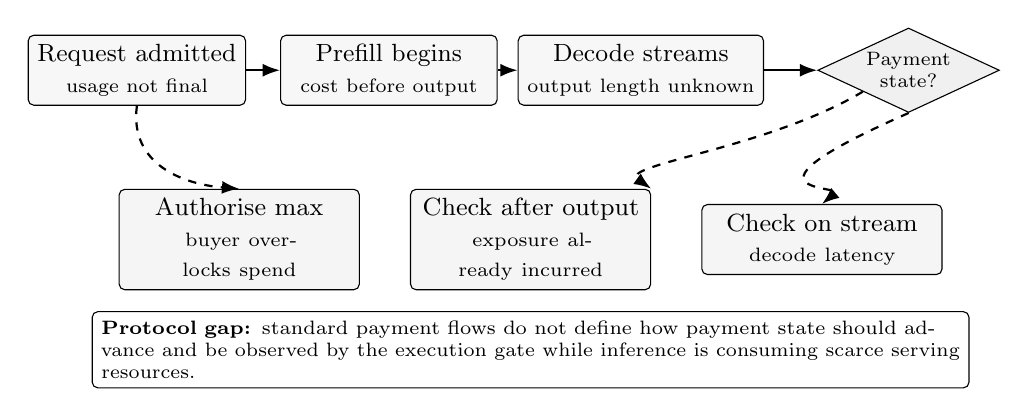
\begin{tikzpicture}[x=1cm,y=1cm]
  \node[process, minimum width=2.75cm] (admit) at (-5.0,0) {Request admitted\\\scriptsize usage not final};
  \node[process, minimum width=2.75cm] (prefill) at (-1.8,0) {Prefill begins\\\scriptsize cost before output};
  \node[process, minimum width=2.75cm] (decode) at (1.4,0) {Decode streams\\\scriptsize output length unknown};
  \node[decision, minimum width=2.25cm] (pay) at (4.8,0) {Payment\\\scriptsize state?};

  \draw[flow] (admit.east) -- (prefill.west);
  \draw[flow] (prefill.east) -- (decode.west);
  \draw[flow] (decode.east) -- (pay.west);

  \node[system, minimum width=3.05cm, text width=2.75cm] (risk) at (0,-2.15) {Check after output\\\scriptsize exposure already incurred};
  \node[system, minimum width=3.05cm, text width=2.75cm] (cap) at (-3.7,-2.15) {Authorise max\\\scriptsize buyer over-locks spend};
  \node[system, minimum width=3.05cm, text width=2.75cm] (stall) at (3.7,-2.15) {Check on stream\\\scriptsize decode latency};

  \draw[riskflow] (pay.south west) .. controls (3.0,-1.0) and (1.1,-1.2) .. (risk.north east);
  \draw[riskflow] (pay.south) .. controls (2.4,-1.6) and (4.0,-1.45) .. (stall.north);
  \draw[riskflow] (admit.south) .. controls (-5.1,-1.2) and (-4.4,-1.45) .. (cap.north);

  \node[note, text width=10.9cm] at (0,-3.55)
    {\textbf{Protocol gap:} standard payment flows do not define how payment state should advance and be observed by the execution gate while inference is consuming scarce serving resources.};
\end{tikzpicture}
\caption{The streaming inference payment problem. The provider incurs prefill and decode cost before the final metered amount due is known, while payment checks that are too late, too large, or placed on the occupied output stream each create a different failure mode.}
\label{fig:inference-payment-gap}
\end{figure}

\section{The Inference Payment Trilemma}

The central trade-off is a trilemma. A naive protocol cannot maximise all three goals:

\begin{enumerate}
  \item Low TTFT and uninterrupted streaming.
  \item Exact final payment for actual usage.
  \item Hard-bounded or risk-budgeted provider exposure and no buyer over-authorisation.
\end{enumerate}

If the provider streams first and settles later, the buyer gets low latency and actual-usage settlement, but the provider accepts maximum unpaid admitted work that is not constrained by payment state. If the provider requires a high maximum authorisation before execution, unpaid work is constrained and streaming can proceed, but the buyer over-authorises against a worst case. If the provider requires payment at very fine token boundaries on the same occupied output path, the buyer and provider can keep unpaid work small in theory, but payment-control latency enters the decode path and can degrade streaming.

The trilemma is an engineering trade-off, not an impossibility theorem. Fixed prices work for small bounded calls. Subscriptions and prepaid balances work inside durable commercial relationships. High \field{upto} caps work when buyers tolerate capital lock-up. The claim here is specific: open-ended streamed inference needs explicit execution semantics to keep bilateral risk either hard-bounded under deterministic profiles or risk-budgeted under disclosed quantile profiles without putting payment in the per-token critical path.

\section{Design Goals and Out of Scope}

\subsection{Goals}

\begin{enumerate}
  \item \textbf{Bound unpaid admitted work.} A provider should know the unpaid compute it can admit for a run under the selected risk-budget or hard-bound profile.
  \item \textbf{Bound buyer authorisation.} A buyer should authorise spend according to policy rather than sign a large worst case amount for every request.
  \item \textbf{Protect streaming quality.} Top-up cadence should be designed and measured so it does not stall decode or materially increase TTFT under expected operating conditions.
  \item \textbf{Stay compatible with MPP.} \mppi{} should use MPP's challenge, credential, and receipt model while defining lifecycle semantics for inference through a proposed \field{inference} intent or profile.
  \item \textbf{Keep settlement method flexibility.} \mppi{} should not mandate a settlement rail, asset, processor, or single facilitator. The selected payment method compatible with MPP should carry or settle the payment while \mppi{} defines inference semantics.
  \item \textbf{Make receipts auditable without exposing inference content.} Final receipts should reconcile request commitments, delivered unit commitments, usage, timing, metered amount due, and settlement references without putting raw prompt, raw output, or raw transcript on the payment plane.
  \item \textbf{Define termination explicitly.} Low credit should lead to defined states such as \field{low_credit}, \field{draining}, \field{stopped}, and \field{settled}; not an ambiguous pause.
\end{enumerate}

\subsection{Out of Scope}

\begin{enumerate}
  \item \textbf{No semantic output quality guarantee.} Base \mppi{} can receipt what was run and metered; it cannot prove the answer was useful or correct.
  \item \textbf{No mandatory settlement method.} The protocol should not require a settlement rail, asset, processor, or single facilitator.
  \item \textbf{No universal pricing policy.} Providers set prices. \mppi{} standardises how prices and billable units are represented.
  \item \textbf{No full dispute court.} The base layer should support evidence for disputes, not adjudicate subjective output quality.
  \item \textbf{No requirement for token-synchronous payment.} Payment authorisation should be ahead of execution, metered cumulatively, and refreshed at coarse enough intervals to preserve serving performance.
\end{enumerate}


\section{Proposed Solution Overview}

\mppi{} turns payment state into an explicit inference payment synchronisation contract. The protocol does not require a specific settlement rail, asset, processor, or facilitator. Instead, it defines the objects and state transitions that connect an MPP payment authorisation to an inference run.

\subsection{Target Architecture}

Figure~\ref{fig:mppi-architecture} separates the inference plane from the payment/control plane. The inference plane carries the request payload and streamed inference output. The payment/control plane carries quote and policy state, reservations scoped to the run, cumulative credit grants, signed meter frames, low-credit and drain events, cancellation, settlement references, and receipts. The payment/control plane must never carry raw prompt, raw output, or raw transcript. The provider gateway verifies admission, but the decisive enforcement point is the scheduler or worker admission gate: no new billable interval should enter the serving path unless the current payment state covers the next disclosed interval.



\begin{figure}[H]
\centering
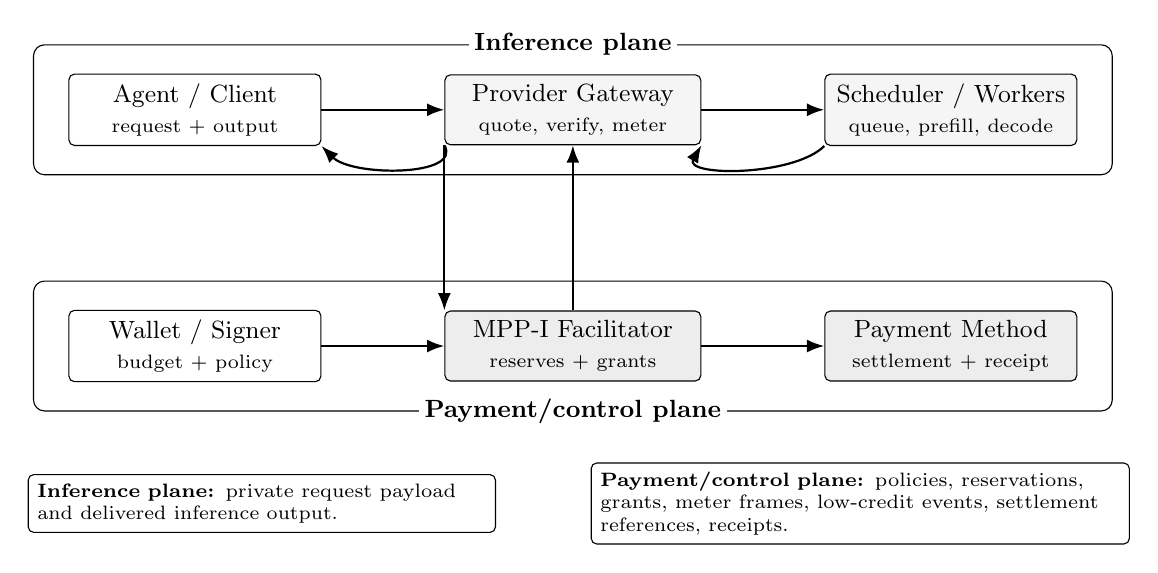
\begin{tikzpicture}[x=1cm,y=1cm]
  \node[draw, rounded corners=4pt, minimum width=13.7cm, minimum height=1.65cm] (infbox) at (0,0) {};
  \node[font=\small\bfseries, fill=white, inner sep=2pt] at (infbox.north) {Inference plane};

  \node[draw, rounded corners=4pt, minimum width=13.7cm, minimum height=1.65cm] (paybox) at (0,-3.0) {};
  \node[font=\small\bfseries, fill=white, inner sep=2pt] at (paybox.south) {Payment/control plane};

  \node[actor, minimum width=3.2cm] (agent) at (-4.8,0) {Agent / Client\\\scriptsize request + output};
  \node[system, minimum width=3.25cm] (gateway) at (0,0) {Provider Gateway\\\scriptsize quote, verify, meter};
  \node[system, minimum width=3.2cm] (scheduler) at (4.8,0) {Scheduler / Workers\\\scriptsize queue, prefill, decode};

  \node[actor, minimum width=3.2cm] (wallet) at (-4.8,-3.0) {Wallet / Signer\\\scriptsize budget + policy};
  \node[rail, minimum width=3.25cm] (facilitator) at (0,-3.0) {\mppi{} Facilitator\\\scriptsize reserves + grants};
  \node[rail, minimum width=3.2cm] (method) at (4.8,-3.0) {Payment Method\\\scriptsize settlement + receipt};

  \draw[dataflow] (agent.east) -- (gateway.west);
  \draw[dataflow] (gateway.east) -- (scheduler.west);
  \draw[dataflow] (scheduler.south west) .. controls (2.8,-0.85) and (1.4,-0.85) .. (gateway.south east);
  \draw[dataflow] (gateway.south west) .. controls (-1.4,-0.85) and (-2.8,-0.85) .. (agent.south east);

  \draw[payflow] (wallet.east) -- (facilitator.west);
  \draw[payflow] (facilitator.east) -- (method.west);
  \draw[payflow] (facilitator.north) -- (gateway.south);
  \draw[payflow] (gateway.south west) -- (facilitator.north west);

  \node[note, text width=5.7cm] at (-3.95,-5.0)
    {\textbf{Inference plane:} private request payload and delivered inference output.};
  \node[note, text width=6.6cm] at (3.65,-5.0)
    {\textbf{Payment/control plane:} policies, reservations, grants, meter frames, low-credit events, settlement references, receipts.};
\end{tikzpicture}

\vspace{0.35em}
\footnotesize
\begin{tabularx}{0.92\linewidth}{>{\bfseries\raggedright\arraybackslash}p{0.24\linewidth} >{\raggedright\arraybackslash}X}
Inference messages & Agent sends a private request; scheduler output returns through the provider gateway. \\
Payment messages & Wallet policy flows to the facilitator; grants flow to the gateway; delivery acknowledgements and meter frames reconcile delivered output with billable usage. \\
Execution gate & New billable work may enter the scheduler or worker queue only while available amount covers required headroom at the disclosed metering boundary. \\
Privacy boundary & Raw prompt, raw output, and raw transcript stay off the payment/control plane. \\
\end{tabularx}
\caption{Proposed \mppi{} architecture: inference delivery remains separate from payment-control authorisation, but both meet at the provider's scheduler or worker admission gate.}
\label{fig:mppi-architecture}
\end{figure}

\subsection{End-to-End Run Lifecycle}

Figure~\ref{fig:mppi-facilitated-swimlane} shows the facilitated run as a sequence across the agent, wallet, facilitator, provider gateway, scheduler, and settlement path. Figure~\ref{fig:mppi-run-lifecycle} summarises the same lifecycle as operational steps. Direct mode removes the facilitator but keeps the same quote, policy, grant, meter, payment state, and receipt semantics. Payment authorisation is necessary for an \mppi{} run, but it is not the same as scheduler admission. A queued run should carry the payment-state version and grant sequence that authorised it, and the provider should revalidate that state before the run becomes scheduler-admitted work.

\begin{figure}[H]
\centering
\resizebox{0.99\linewidth}{!}{%
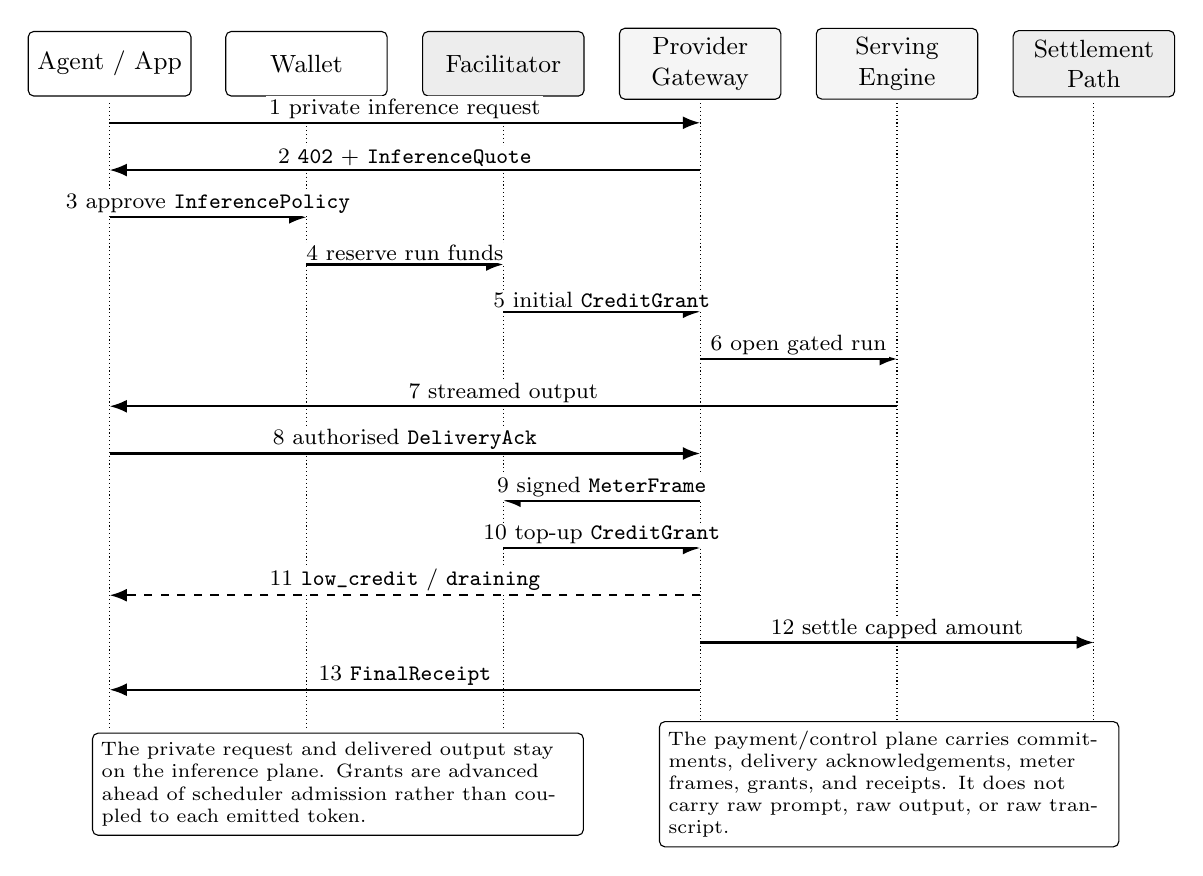
\begin{tikzpicture}[x=1cm,y=1cm, font=\footnotesize]
  \node[actor, minimum width=2.05cm] (agent) at (-6.2,0) {Agent / App};
  \node[actor, minimum width=2.05cm] (wallet) at (-3.7,0) {Wallet};
  \node[rail, minimum width=2.05cm] (fac) at (-1.2,0) {Facilitator};
  \node[system, minimum width=2.05cm] (gateway) at (1.3,0) {Provider\\Gateway};
  \node[system, minimum width=2.05cm] (sched) at (3.8,0) {Serving\\Engine};
  \node[rail, minimum width=2.05cm] (settle) at (6.3,0) {Settlement\\Path};

  \foreach \x in {-6.2,-3.7,-1.2,1.3,3.8,6.3} {
    \draw[densely dotted] (\x,-0.5) -- (\x,-8.45);
  }

  \draw[flow] (-6.2,-0.75) -- node[above, fill=white, inner sep=1pt] {1 private inference request} (1.3,-0.75);
  \draw[flow] (1.3,-1.35) -- node[above, fill=white, inner sep=1pt] {2 \field{402} + \field{InferenceQuote}} (-6.2,-1.35);
  \draw[flow] (-6.2,-1.95) -- node[above, fill=white, inner sep=1pt] {3 approve \field{InferencePolicy}} (-3.7,-1.95);
  \draw[flow] (-3.7,-2.55) -- node[above, fill=white, inner sep=1pt] {4 reserve run funds} (-1.2,-2.55);
  \draw[flow] (-1.2,-3.15) -- node[above, fill=white, inner sep=1pt] {5 initial \field{CreditGrant}} (1.3,-3.15);
  \draw[flow] (1.3,-3.75) -- node[above, fill=white, inner sep=1pt] {6 open gated run} (3.8,-3.75);
  \draw[flow] (3.8,-4.35) -- node[above, fill=white, inner sep=1pt] {7 streamed output} (-6.2,-4.35);
  \draw[payflow] (-6.2,-4.95) -- node[above, fill=white, inner sep=1pt] {8 authorised \field{DeliveryAck}} (1.3,-4.95);
  \draw[payflow] (1.3,-5.55) -- node[above, fill=white, inner sep=1pt] {9 signed \field{MeterFrame}} (-1.2,-5.55);
  \draw[payflow] (-1.2,-6.15) -- node[above, fill=white, inner sep=1pt] {10 top-up \field{CreditGrant}} (1.3,-6.15);
  \draw[riskflow] (1.3,-6.75) -- node[above, fill=white, inner sep=1pt] {11 \field{low_credit} / \field{draining}} (-6.2,-6.75);
  \draw[flow] (1.3,-7.35) -- node[above, fill=white, inner sep=1pt] {12 settle capped amount} (6.3,-7.35);
  \draw[flow] (1.3,-7.95) -- node[above, fill=white, inner sep=1pt] {13 \field{FinalReceipt}} (-6.2,-7.95);

  \node[note, text width=6.0cm] at (-3.3,-9.15)
    {The private request and delivered output stay on the inference plane. Grants are advanced ahead of scheduler admission rather than coupled to each emitted token.};
  \node[note, text width=5.6cm] at (3.7,-9.15)
    {The payment/control plane carries commitments, delivery acknowledgements, meter frames, grants, and receipts. It does not carry raw prompt, raw output, or raw transcript.};
\end{tikzpicture}%
}
\caption{Facilitated \mppi{} run sequence. MPP provides the \field{402} payment envelope; \mppi{} keeps run-scoped credit, metering, and control messages parallel to the private inference stream and visible to the scheduler admission gate.}
\label{fig:mppi-facilitated-swimlane}
\end{figure}


\begin{figure}[H]
\centering
\footnotesize
\setlength{\tabcolsep}{3.5pt}
\begin{tabularx}{\linewidth}{>{\bfseries\raggedright\arraybackslash}p{0.07\linewidth} >{\raggedright\arraybackslash}p{0.21\linewidth} >{\raggedright\arraybackslash}X >{\raggedright\arraybackslash}p{0.25\linewidth}}
\toprule
Step & Actor & Message or action & Execution effect \\
\midrule
1 & Agent $\rightarrow$ Provider & Send private inference request with inference target, context, output bound, and request commitment. & Provider may tokenise and price prefill; no serving-engine execution. \\
2 & Provider $\rightarrow$ Agent & Return \field{402} challenge with \field{InferenceQuote}: inference target, tokenizer version, serialisation profile, unit prices, prefill bound, recommended reservation, starting authorisation, watermarks, admitted-interval policy, accepted payment methods, and expiry. & Defines executable offer. \\
3 & Agent $\rightarrow$ Wallet & Sign \field{InferencePolicy} bound to quote, request commitment, max spend, payment method, destination, allowed units, and expiry. & Buyer policy becomes verifiable by machine. \\
4 & Wallet / Facilitator & Reserve or lock claimable funds for the run. & Prevents double spend across runs. \\
5 & Facilitator $\rightarrow$ Provider & Send initial cumulative \field{CreditGrant}. & Covers \field{required_initial_credit}: prefill plus first decode headroom. \\
6 & Provider $\rightarrow$ Scheduler & Queue the run with payment-state version, then revalidate before scheduler admission. & Prefill and decode may enter the serving path only while headroom holds. \\
7 & Provider $\rightarrow$ Agent / client transport endpoint & Stream output on the inference plane. & Delivered output is sequenced under the selected transport profile. \\
8 & Authorised acknowledgement role $\rightarrow$ Provider & Send signed \field{DeliveryAck} for the delivered range under the acknowledgement authority named in the quote and policy. & In the acknowledged-billable profile, output amount due may advance only up to the latest accepted acknowledgement. \\
9 & Provider $\rightarrow$ Facilitator / Wallet & Emit signed cumulative \field{MeterFrame} records. & Billable output is separated from any delivered but unacknowledged range, and non-output units remain explicit billable events. \\
10 & Facilitator $\rightarrow$ Provider & Send top-up grants before the low or drain-entry watermark and before the next per-run admitted interval. & Decode continues without token-synchronous payment. \\
11 & Provider & Emit \field{low_credit}; drain through already authorised headroom; stop or settle by policy if no valid top-up arrives. & Budget exhaustion follows the disclosed boundary policy. \\
12 & Provider $\rightarrow$ Payment Method / Agent & Settle the cumulative metered amount due up to the latest valid cumulative grant, client policy, and run claimable limit; emit \field{FinalReceipt}. & Usage, commitments, amount, and settlement reference reconcile. \\
\bottomrule
\end{tabularx}
\caption{Proposed \mppi{} facilitated run lifecycle. Grants and meter frames are cumulative so reconnects and retries do not double count payment state.}
\label{fig:mppi-run-lifecycle}
\end{figure}

A wallet receives raw output only when the quote and policy explicitly designate it as the client-side receiver or transport adapter. A wallet that only signs spend policy or credit grants remains on the payment/control plane and should not be treated as the raw-output recipient or factual delivery observer by default. A wallet or facilitator may sign \field{DeliveryAck} only when the quote and policy designate it as acknowledgement authority for a concrete transport boundary. If it observes raw output to make that acknowledgement, it is acting as an inference-plane receiver or transport adapter for that purpose, not as a control-plane-only wallet or facilitator.

\subsection{What Changes Relative to Today}

Table~\ref{tab:mppi-changes-relative} summarises the practical shift from current payment flows to the proposed \mppi{} flow.

\begin{table}[H]
\centering
\caption{Current state flow versus proposed \mppi{} flow}
\label{tab:mppi-changes-relative}
\begin{tabularx}{\linewidth}{>{\bfseries\raggedright\arraybackslash}p{0.21\linewidth} >{\raggedright\arraybackslash}X >{\raggedright\arraybackslash}X}
\toprule
Dimension & Today & With \mppi{} \\
\midrule
Admission & Provider-specific balance, fixed charge, or request cap. & Executable quote plus initial grant covering prefill and first decode headroom. \\
Streaming & Provider-specific policy for meter cadence and low balance. & Signed cumulative meter frames and disclosed low/drain-entry watermarks. \\
Top-up & Manual, account-specific, or hidden inside a generic session. & Cumulative credit grants bound to run, policy, quote, sequence, payment method, and meter acknowledgement. \\
Low credit & Ambiguous: TCP backpressure, scheduler pause, cache retention, truncation, or abort may be conflated. & Explicit \field{low_credit}, \field{draining}, \field{stopped}, \field{settlement_pending}, and \field{settled} states. \\
Settlement & Final settlement is specific to the payment method and may be hard to reconcile with streamed output. & Final receipt reconciles request commitment, delivered unit commitments, billable event commitments, usage, metered amount due, \field{settlement_target_amount}, \field{settled_amount}, and settlement reference. \\
Risk bound & Depends on provider-specific heuristics. & Hard-bounded under deterministic profiles, or risk-budgeted under disclosed quantile profiles with explicit tail-overrun handling. \\
\bottomrule
\end{tabularx}
\end{table}

\section{Protocol Model}

\subsection{Actors}

\begin{longtable}{>{\raggedright\arraybackslash}p{0.24\linewidth} >{\raggedright\arraybackslash}p{0.68\linewidth}}
\caption{Core actors}\label{tab:core-actors}\\
\toprule
\textbf{Actor} & \textbf{Role} \\
\midrule
\endfirsthead
\toprule
\textbf{Actor} & \textbf{Role} \\
\midrule
\endhead
Client or agent & Requests inference, evaluates quotes, obtains payment authorisation, receives stream and receipt. \\
Wallet or delegated signer & Enforces user spend policy and signs bounded payment authorisations or credit grants. \\
Facilitator & Optionally reserves funds, verifies policies, issues grants that providers can verify, prevents double spend across runs, and batches settlement. \\
Provider gateway & Verifies quote and payment state, opens runs, emits inference plane and payment/control messages, and coordinates settlement. \\
Inference scheduler & Executes prefill and decode only while payment state permits. \\
Payment method or settlement path & Moves value or enforces claimability under the selected MPP payment method. Examples include charge style stablecoin methods, settlement context compatible with x402, MPP session vouchers, or credit assurances backed by a facilitator. \\
\bottomrule
\end{longtable}

\subsection{Two Logical Planes}

\mppi{} should define logical behaviour rather than requiring a single transport in the paper-level protocol. The front matter defines this paper's non-normative language convention; formal conformance requirements belong in the eventual profile specification once it fixes exact schemas, transport mapping, and settlement method behaviour.

\textbf{Inference plane.} The provider receives the private inference request and streams delivered output units such as text tokens, tool call outputs, or multimodal outputs. This plane may carry raw prompt and raw output between client and provider, subject to the provider's privacy and security commitments.

\textbf{Payment/control plane.} The client, wallet, or facilitator opens a run, reserves or locks claimable funds, submits initial credit, sends top-up credit grants, receives signed meter frames, receives low-credit and drain events, cancels, and receives settlement references and final receipts. This plane carries only policy, accounting, and content-private commitments. It must not carry raw prompt, raw output, or raw transcript.

\begin{figure}[H]
\centering
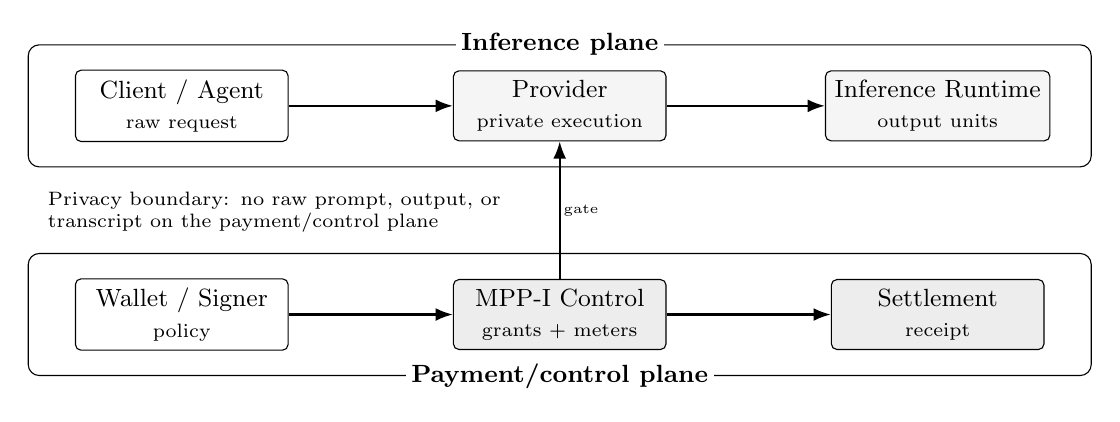
\begin{tikzpicture}[x=1cm,y=1cm]
  \node[draw, rounded corners=4pt, minimum width=13.5cm, minimum height=1.55cm] (inf) at (0,0) {};
  \node[font=\small\bfseries, fill=white, inner sep=2pt] at (inf.north) {Inference plane};
  \node[actor, minimum width=2.7cm] (client) at (-4.8,0) {Client / Agent\\\scriptsize raw request};
  \node[system, minimum width=2.7cm] (provider) at (0,0) {Provider\\\scriptsize private execution};
  \node[system, minimum width=2.7cm] (model) at (4.8,0) {Inference Runtime\\\scriptsize output units};

  \node[draw, rounded corners=4pt, minimum width=13.5cm, minimum height=1.55cm] (pay) at (0,-2.65) {};
  \node[font=\small\bfseries, fill=white, inner sep=2pt] at (pay.south) {Payment/control plane};
  \node[actor, minimum width=2.7cm] (wallet2) at (-4.8,-2.65) {Wallet / Signer\\\scriptsize policy};
  \node[rail, minimum width=2.7cm] (control) at (0,-2.65) {\mppi{} Control\\\scriptsize grants + meters};
  \node[rail, minimum width=2.7cm] (receipt2) at (4.8,-2.65) {Settlement\\\scriptsize receipt};

  \draw[dataflow] (client.east) -- (provider.west);
  \draw[dataflow] (provider.east) -- (model.west);
  \draw[payflow] (wallet2.east) -- (control.west);
  \draw[payflow] (control.east) -- (receipt2.west);
  \draw[payflow] (control.north) -- node[right, font=\tiny, fill=white, inner sep=1pt] {gate} (provider.south);
  \node[font=\scriptsize, text width=5.8cm, align=left] at (-3.6,-1.35) {Privacy boundary: no raw prompt, output, or transcript on the \mbox{payment/control} plane};
\end{tikzpicture}
\caption{Two logical planes and the privacy boundary. The payment/control plane can bind to delivered unit and billable event commitments without seeing inference content.}
\label{fig:mppi-privacy-boundary}
\end{figure}

The planes may run over WebSocket, HTTP/2 streams, gRPC, SSE plus POST, HTTP/3, WebTransport, or another transport. What matters is that control messages are ordered, protected against replay, bound to the run, and visible to the provider's scheduler or worker admission gate before compute continues beyond the covered metering boundary.

Independent streams still need application-level sequencing. Delivered output should have a monotonically increasing delivered sequence. Meter frames should state the delivered sequence range and any separate billable event range they cover. Credit grants should acknowledge the latest accepted meter frame sequence. When output billing uses \field{acknowledged_delivered_output}, credit grants after the initial grant should also carry the latest acknowledged delivered sequence or range used by the payer, wallet, facilitator, or transport adapter. Low credit, draining, stop, cancellation, and final receipt messages should also be sequenced and bound to the run. On reconnect, both sides resume from the highest mutually accepted meter frame and the latest accepted cumulative grant; duplicate messages are idempotent, and older grants cannot reduce the latest accepted authorisation.

\begin{table}[H]
\centering
\caption{Delivery terminology}
\label{tab:delivery-terminology}
\footnotesize
\begin{tabularx}{\linewidth}{>{\bfseries\raggedright\arraybackslash}p{0.34\linewidth} >{\raggedright\arraybackslash}X}
\toprule
Term & Meaning \\
\midrule
\field{generated_output} & Output produced by the inference runtime. \\
\field{emitted_output} & Output handed from the runtime or serving engine to the provider transport layer. \\
\field{transport_flushed_output} & Output written or flushed to the transport. \\
\field{delivered_sequence} & Signed, ordered sequence of output units presented to the client side under the transport profile. \\
\field{acknowledged_delivered_output} & Delivered sequence acknowledged at the application-layer boundary named by the quote, policy, and transport profile. \\
\bottomrule
\end{tabularx}
\end{table}

Each transport profile must define what \emph{delivered} means. The default billable output boundary should be \field{acknowledged_delivered_output}: output included in a signed delivered sequence and acknowledged at the application layer by the client, or by a wallet, facilitator, or transport adapter that the quote and policy explicitly authorise to acknowledge that delivery boundary. A wallet or facilitator that does not observe the output or the relevant transport boundary should not be treated as acknowledging delivered content except as an authorised proxy for a client-side or transport-adapter acknowledgement. For the base text-output profile, output may enter \field{cumulative_amount_due} only when it is in a signed delivered sequence at or below the latest accepted \field{DeliveryAck} for the run. Delivered but unacknowledged output should be reported separately from billable output or remain provider risk. A profile may use a weaker boundary, such as server flush or socket write, only if that choice is disclosed in the quote and policy; weaker delivery semantics shift dispute risk and should not be hidden behind the word delivered.

Transport profiles should also define the operational limits that keep delivered-output billing unambiguous: flow-control windows, maximum buffered bytes or output units, acknowledgement cadence, maximum unacknowledged delivered range or acknowledgement-lag range, slow-consumer policy, half-close behaviour, reconnect state, and whether acknowledgement is made by the application, wallet, facilitator, or transport adapter. Per-output acknowledgements may be too expensive for low inter-token latency, so profiles should choose an acknowledgement cadence that keeps dispute exposure constrained without putting acknowledgement on the critical path of every decode iteration. If a client exceeds the maximum buffered output or maximum acknowledgement-lag range, the provider should apply the disclosed slow-consumer policy: emit \field{ack_lag_low} or \field{ack_lag_exceeded}, pause emission, or stop at the next enforceable delivery boundary. Output beyond the acknowledged delivered range is provider risk unless the quote and policy disclosed a weaker delivery boundary.

When \field{acknowledged_delivered_output} is the billing boundary, acknowledgement should be a first-class signed \field{DeliveryAck}, not only an implied side effect of a grant or transport read. A \field{DeliveryAck} binds the authorised acknowledgement role, delivered range, delivered-unit commitment, meter-frame reference where one exists, and signer to the run without exposing raw output on the payment/control plane. Meter frames that advance output amount due should reference the accepted \field{DeliveryAck} sequence or hash. Meter frames may also report a delivered but unbilled range so the client and provider can reconcile slow consumers, reconnects, and final stops without treating unacknowledged output as billable output. Profiles should also define signed and sequenced \field{Resume}, \field{Cancel}, \field{Stop}, and terminal messages. Those messages need a state vector covering the latest delivered sequence, latest accepted \field{DeliveryAck} sequence and hash where used, latest accepted meter frame sequence and hash, latest accepted grant sequence and hash, control message sequence, and terminal state if one exists. Race precedence should be explicit: terminal settlement closes the run, stale top-ups cannot reopen it, stale cancels cannot erase already admitted metered work, and duplicate terminal messages settle idempotently against the same run and payment path.

\subsection{High Performance Transport Example}

\mppi{} is aware of transport profiles, but it is not prescriptive about transport. A low-latency serving profile can expose an HTTP endpoint compatible with MPP for payment admission and then run the inference session over independent HTTP/2 or gRPC streams:

\begin{enumerate}
  \item The agent requests inference. The provider replies with an MPP \field{402} challenge carrying an \mppi{} quote.
  \item The client or inference wallet approves a policy and submits the initial authorisation for the run.
  \item The provider starts the run and opens one stream for delivered inference output and another independent stream for payment/control messages.
  \item The client, wallet, facilitator, or transport adapter authorised by the policy signs \field{DeliveryAck} messages for delivered ranges under the selected acknowledgement cadence.
  \item The provider emits signed cumulative meter frames at disclosed boundaries. In the acknowledged-billable profile, output amount due advances only through the latest accepted \field{DeliveryAck}. The wallet or facilitator responds with cumulative credit grants before the drain-entry watermark is reached.
  \item If grants stop arriving, the provider drains only through already authorised headroom, emits \field{draining}, stops at the disclosed boundary, settles the final amount up to the latest valid cumulative grant, client policy, and run claimable limit, and emits a final receipt.
\end{enumerate}

This shape avoids token-synchronous payments. Grant verification must fit within the profile's p99 grant-verification budget, while the execution gate only needs to know whether available amount covers the next disclosed billable interval. The same transport-independent protocol lifecycle can be carried over SSE plus a side-channel POST endpoint, WebSocket, or HTTP/3/QUIC/WebTransport when those transports preserve ordering, replay protection, run binding, flow control, acknowledgement semantics, and the privacy boundary between inference content and payment metadata.

\subsection{Payment Synchronisation State}

Payment synchronisation state is run-level accounting state local to the provider unless a transport profile explicitly exposes part of it. Every quantity used in the execution gate should be denominated in the smallest unit of the selected payment or settlement method. Tokens, time, tool units, multimodal units, reasoning tokens, cached input, KV hold intervals, and scheduler-admitted accelerator intervals may be billable unit types only when explicitly quoted, metered, and receipted. They must be converted through the quoted price schedule and rounded up before comparison.

Provider-observed units and units that are not output require a stronger verification regime than visible output tokens. The base paper requires them to be quoted, admitted, metered, and receipted, but it does not make them independently verifiable. A formal profile should declare the provider assumption, or add an attestation profile, audit process, or dispute-opening mechanism, before claiming independent verifiability for reasoning tokens, internal compute, KV hold time, or scheduler-admitted accelerator time.

\begin{table}[H]
\centering
\caption{Billable unit verifiability}
\label{tab:billable-unit-verifiability}
\footnotesize
\begin{tabularx}{\linewidth}{>{\raggedright\arraybackslash}p{0.20\linewidth} >{\raggedright\arraybackslash}p{0.22\linewidth} >{\raggedright\arraybackslash}p{0.25\linewidth} >{\raggedright\arraybackslash}X}
\toprule
\textbf{Unit} & \textbf{Visibility} & \textbf{Meter evidence} & \textbf{Profile status} \\
\midrule
Input / prefill tokens & Reproducible when the serialisation surface is bound. & Tokenizer version, chat template or serialisation profile, input-token count, request commitment. & Base profile, exact or conservative before prefill. \\
Delivered output & Client-visible when delivered and acknowledged under the transport profile. & Signed delivered sequence range, meter frame, acknowledgement reference. & Base profile. \\
Cached input & Provider-observed unless the cache hit is committed before admission. & Cache-hit class, cache scope, fallback miss rule, corrected quote when needed. & Advanced or explicitly disclosed profile. \\
External tool units & Visible to the tool endpoint or third party when receipted. & Tool request commitment, tool receipt, meter frame. & Advanced or third-party receipted profile. \\
Reasoning or internal compute & Provider-observed. & Provider-signed meter, optional audit or attestation. & Advanced profile only. \\
KV hold interval & Provider-observed. & Scope, token span, residency tier, start/end time, eviction and recompute policy. & Advanced profile only. \\
Accelerator interval & Provider-observed or attested. & Scheduler-admitted interval, timing policy, optional attestation. & Advanced or attestation profile. \\
\bottomrule
\end{tabularx}
\end{table}

For the base profile, amount due is boundary-posted. Let \(A_t\) denote latest accepted cumulative authorisation, \(A_t^{\mathrm{valid}}\) the portion of that authorisation that is valid for the relevant decision point under the grant-validity and settlement-method rules, \(P_t\) boundary-posted cumulative amount due, and \(\mathcal{I}_t\) the set of active admitted intervals that have not yet reached their metering boundary. The execution gate must use only currently claimable, policy-valid run funds:

\[
A_t^{\mathrm{gate}}=
\min(A_t^{\mathrm{valid}},\mathrm{policy\_max\_total},\mathrm{run\_claimable\_limit}_t)
\]

If a profile already defines \(A_t\) as a provider-verified, valid, policy-clamped, run-claimable amount, then \(A_t^{\mathrm{gate}}=A_t\). Otherwise, \(A_t^{\mathrm{gate}}\) is the amount used by admission and finish gates. A signed grant that is expired for the relevant decision point, not accepted under the causal grant rule, or not backed by current run claimability cannot increase \(A_t^{\mathrm{gate}}\). Each interval \(i \in \mathcal{I}_t\) has an admitted maximum cost \(C_i^{\max}\). The provider computes:

\[
\begin{aligned}
B_{\mathrm{active},t} &= \sum_{i \in \mathcal{I}_t} C_i^{\max}\\
a_t &= A_t^{\mathrm{gate}} - P_t - B_{\mathrm{active},t}\\
a_{t,i}^{\mathrm{finish}} &= A_t^{\mathrm{gate}} - P_t - (B_{\mathrm{active},t} - C_i^{\max})
\end{aligned}
\]

Here, \field{posted_cumulative_amount_due} is the provider-local name for the accrued billable amount for the run that has reached disclosed metering boundaries. The canonical wire-facing field name in signed meter frames and receipt bindings is \field{cumulative_amount_due}; it means the same boundary-posted amount, not provisional generated usage. A profile must not give \field{posted_cumulative_amount_due} and \field{cumulative_amount_due} divergent semantics. For output under the base text-output profile, this amount advances only for output covered by the selected delivery and acknowledgement boundary. Non-output units advance it only when they are separately quoted, admitted, metered, and represented as billable events.

Candidate admission uses a hypothetical post-admission active set. For candidate interval \(j\), define:

\[
\begin{aligned}
\mathcal{I}_t^{+j} &= \mathcal{I}_t \cup \{j\}\\
B_{\mathrm{active},t}^{+j} &= B_{\mathrm{active},t} + C_j^{\max}\\
a_{t,i}^{\mathrm{finish},+j} &= A_t^{\mathrm{gate}} - P_t - (B_{\mathrm{active},t}^{+j} - C_i^{\max}), \quad i \in \mathcal{I}_t^{+j}
\end{aligned}
\]

The ordinary \(a_{t,i}^{\mathrm{finish}}\) value is used for intervals that are already admitted. The \(+j\) value is used only to test whether all intervals that would be active after admitting candidate \(j\) remain finishable.

Grant validity and method claimability must be evaluated at explicit decision points. A profile should define whether \field{valid_until}, policy expiry, and settlement-method claimability are checked at candidate admission, interval finish, meter posting, settlement submission, finality, or all of those points. The base paper rule is conservative: a candidate interval may be admitted only if the accepted grant and method claimability are valid for the interval's disclosed boundary or the method profile creates a run-scoped claimability snapshot that remains enforceable through that boundary. If the payment method cannot prove claimability through the boundary, the provider must shorten the interval, request fresh authorisation, or stop before admitting it. The \field{active_admitted_interval} record should therefore snapshot the grant sequence, cumulative authorised amount, grant validity or claimability evidence, payment-state version, run-claimable limit used for the gate, and settlement-method reference needed to verify the final receipt.

Each admitted interval must also map back to the executable quote. The interval's \(C_j^{\max}\) should be computed from a named quote line item, metering-boundary profile, billable unit type, unit-count or time bound, price schedule, rounding rule, and any evidence profile used for non-output units. The \field{maximum_cost} in the interval record is that computed \(C_j^{\max}\), expressed in the smallest payment unit. The quote-level \(C_{\mathrm{next},t}^{\max}\) should be either a derived alias for the next candidate interval's computed \(C_j^{\max}\), or a disclosed maximum-admitted-interval cap that every candidate \(C_j^{\max}\) must not exceed. A verifier should be able to reconstruct this mapping from the quote, policy, meter frame, and final receipt without seeing raw prompt or raw output.

The base transition order is explicit:

\begin{enumerate}
  \item Apply all accepted grants and already posted meter frames for the run. Compute \(A_t^{\mathrm{gate}}\) from valid accepted authorisation, policy maximum, and current run claimability, then compute \(a_t=A_t^{\mathrm{gate}}-P_t-B_{\mathrm{active},t}\). This pre-admission value is used for \(\mathrm{may\_admit\_new\_interval}_{j,t}\), drain-latch checks for new work, and the credit-state label that existed before the candidate interval is admitted.
  \item For candidate interval \(j\), compute \(C_j^{\max}\), \(H_{j,t}^{\mathrm{admit}(q)}\), the interval's \(H_{j,t}^{\mathrm{finish}(q)}\), and the hypothetical post-admission values \(\mathcal{I}_t^{+j}\), \(B_{\mathrm{active},t}^{+j}\), and \(a_{t,i}^{\mathrm{finish},+j}\). The provider must not admit \(j\) unless the admission gate holds and every interval that would be active after admission remains finishable under its own finish guard.
  \item If admitted, append an \field{active_admitted_interval} record with the interval ID, unit type, quote line item, metering-boundary profile, admitted boundary, unit-count or time bound, maximum cost, rounding rule, pricing reference, evidence profile, latest payment-state version, latest grant, grant-validity or claimability snapshot, latest accepted meter frame, and latest acknowledgement reference where used. Then compute \(a_t^{\mathrm{reserve}(j)}=A_t^{\mathrm{gate}}-P_t-(B_{\mathrm{active},t}+C_j^{\max})\). This post-reservation value may trigger \field{low_credit}, \field{draining}, or no-new-admission state for future intervals, but it does not retroactively invalidate interval \(j\) if the admission and finish guards held at admission.
  \item During execution, \field{posted_cumulative_amount_due} does not advance for interval \(j\) unless the profile defines a stricter continuous-posting rule.
  \item At the disclosed boundary, emit a \field{MeterFrame}, post the actual billable amount to \field{posted_cumulative_amount_due}, remove or reduce the interval's active bound, compute \(a_t^{\mathrm{posted}}\), then recompute \field{credit_state}, acknowledgement state, and drain latch before any further admission.
\end{enumerate}

This separates work that is already due from work that is admitted but still in flight.

\begin{longtable}{>{\bfseries\raggedright\arraybackslash}p{0.18\linewidth} >{\raggedright\arraybackslash}p{0.72\linewidth}}
\caption{Payment synchronisation notation}
\label{tab:payment-sync-notation}\\
\toprule
Symbol & Meaning \\
\midrule
\endfirsthead
\toprule
Symbol & Meaning \\
\midrule
\endhead
\(A_t\) & Latest accepted cumulative authorisation for the run before grant-validity, policy, and claimability clamping. \\
\(A_t^{\mathrm{valid}}\) & Portion of \(A_t\) valid for the relevant decision point under the causal grant, expiry, and settlement-method rules. \\
\(A_t^{\mathrm{gate}}\) & Gate-clamped cumulative authorisation for the run: valid accepted authorisation capped by \field{policy_max_total} and current \field{run_claimable_limit}. Admission and finish gates use this value. \\
\(P_t\) & Boundary-posted cumulative amount due for the run. The provider-local state name is \field{posted_cumulative_amount_due}; the canonical signed field name is \field{cumulative_amount_due}. They are aliases for the same boundary-posted amount. \\
\(\mathcal{I}_t\) & Active admitted intervals not yet posted to due. \\
\(B_{\mathrm{active},t}\) & Sum of maximum cost bounds for active admitted intervals in \(\mathcal{I}_t\). \\
\(a_t\) & Pre-admission available amount for admitting new billable work after applying accepted grants, posted due, and active admitted bounds. \\
\(a_t^{\mathrm{reserve}(j)}\) & Available amount immediately after appending candidate interval \(j\)'s admitted bound. Used for credit-state telemetry and future admission, not to retroactively reject interval \(j\). \\
\(a_t^{\mathrm{posted}}\) & Available amount after a boundary meter frame posts actual due and removes or reduces the active bound for the interval that reached the boundary. \\
\(a_{t,i}^{\mathrm{finish}}\) & Amount available for finishing already admitted interval \(i\), computed while preserving the bounds of other active intervals. \\
\(a_{t,i}^{\mathrm{finish},+j}\) & Hypothetical finish amount for interval \(i\) after candidate interval \(j\) is added to the active set. Used only by the admission predicate. \\
\(H_{j,t}^{\mathrm{admit}(q)}\) & Required admission headroom for candidate interval \(j\) at disclosed profile quantile or conservative target \(q\). If a deterministic profile does not use quantiles, it should define this as the deterministic admission headroom. \\
\(H_{i,t}^{\mathrm{finish}(q)}\) & Required finish headroom for already admitted interval \(i\) at disclosed profile quantile or conservative target \(q\). If a deterministic profile does not use quantiles, it should define this as the deterministic finish headroom. \\
\(H_t^{\mathrm{state}}\) & Scalar credit-state projection at boundary \(t\). It is used only for \(\mathrm{credit\_state}\) labels and does not replace \(H_{j,t}^{\mathrm{admit}(q)}\), \(H_{i,t}^{\mathrm{finish}(q)}\), or interval-specific gate predicates. \\
\(L_t\) & Low watermark at boundary \(t\). \\
\(D_t\) & Money-denominated drain-entry watermark at boundary \(t\): crossing it enters monetary \field{draining}, so no new output-producing or otherwise billable interval is admitted unless credit is restored. The hard stop remains the disclosed metering boundary reached when current headroom can no longer be maintained. \\
\(D_{j,t}\) & Candidate-specific drain-entry threshold for interval \(j\). If a profile has only one drain-entry watermark at boundary \(t\), \(D_{j,t}=D_t\). \\
\(C_{\mathrm{next},t}^{\max}\) & Maximum cost of the next admitted billable interval under the quote and metering boundary. A profile should define it either as an alias for the next candidate's computed \(C_j^{\max}\), or as a maximum-admitted-interval cap that every candidate \(C_j^{\max}\) must not exceed. \\
\(M_{\mathrm{exec}}\) & Money-denominated minimum required headroom, named \field{minimum_execution_buffer} in wire objects. It is authorisation headroom, not a separate fee. \\
\(C_{\mathrm{latency},j,t}^{(q)}\), \(C_{\mathrm{latency},i,t}^{(q)}\) & Profile risk budget for billable cost that can accrue for candidate interval \(j\) or already admitted interval \(i\) while payment/control messages become visible to the execution gate. A profile may define a shared \(C_{\mathrm{latency},t}^{(q)}\) alias only when the same value applies to both roles. \\
\(U_{\mathrm{active},t}\) & Set or vector of quoted billable unit types, rates, and enforced maxima that may accrue before a grant, drain, or stop decision becomes visible to the execution gate. \\
\(R_{\mathrm{unacked},t}\) & Delivered but unacknowledged output range or unit count under the selected transport profile. \\
\(\bar{R}_{\mathrm{unacked}}\) & Maximum permitted delivered-but-unacknowledged output range or unit count for the run, stream, or acknowledgement authority named by the quote and policy. Disabled means \(+\infty\). \\
\(R_{\mathrm{low}}\) & Optional delivered-but-unacknowledged range or unit-count warning threshold. If omitted, the profile has no distinct acknowledgement-lag warning state before \(\bar{R}_{\mathrm{unacked}}\). \\
\(W_R\) & Boolean indicating that \(R_{\mathrm{low}}\) is enabled for acknowledgement-lag warnings. \\
\(\mathcal{U}_{\mathrm{unacked},t}\) & Delivered but unacknowledged priced-unit multiset under the selected delivery boundary, used to compute money-denominated acknowledgement exposure without making those units billable under the base profile. \\
\(E_{\mathrm{unacked},t}\) & Money-denominated exposure from delivered but unacknowledged output. Under the base profile this is provider-risk exposure, not billable amount due. \\
\(\bar{E}_{\mathrm{unacked}}\) & Maximum permitted money-denominated provider-risk exposure from delivered but unacknowledged output under the quote and policy. Disabled means \(+\infty\). \\
\(E_{\mathrm{low}}\) & Optional money-denominated acknowledgement-lag exposure warning threshold. If omitted, the profile has no distinct exposure warning state before \(\bar{E}_{\mathrm{unacked}}\). \\
\(W_E\) & Boolean indicating that \(E_{\mathrm{low}}\) is enabled for acknowledgement-lag warnings. \\
\(\mathrm{ack\_state}_t\) & Delivery-lag state derived from delivered but unacknowledged output range and exposure. It is separate from monetary \(\mathrm{credit\_state}(a_t)\). \\
\(\mathrm{ack\_lag\_ok}_t\) & Boolean guard requiring delivered but unacknowledged output to remain within the profile's disclosed range, buffer, or exposure limits. \\
\(q\) & Disclosed end-to-end measurement quantile, simulation quantile, or conservative composition target used by the profile, such as p99. \\
\(\gamma\) & Disclosed safety factor applied to latency exposure. \\
\(B_{\mathrm{tail},j,t}\), \(B_{\mathrm{tail},i,t}\) & Disclosed tail or retry margin for candidate interval \(j\) or already admitted interval \(i\). A profile may define a shared \(B_{\mathrm{tail},t}\) alias only when the same value applies to both roles. \\
\bottomrule
\end{longtable}

Bare headroom names such as \(H_{j,t}^{\mathrm{admit}}\) and \(H_{i,t}^{\mathrm{finish}}\) are informal aliases only after a quote or deterministic profile fixes \(q\). Gate predicates in this paper use the canonical \(H_{j,t}^{\mathrm{admit}(q)}\) and \(H_{i,t}^{\mathrm{finish}(q)}\) forms.

Before admitting any prefill segment, per-run decode window, accepted speculative-token burst, tool unit, multimodal unit, reasoning step, KV hold interval, or scheduler-admitted accelerator interval that has been explicitly quoted as billable, the provider must compute admission headroom for the candidate interval. In the base paper profile, admission headroom is a disclosed risk budget:

\[
H_{j,t}^{\mathrm{admit}(q)} =
\max\left(
M_{\mathrm{exec}},
\left\lceil
C_j^{\max}
+ \gamma C_{\mathrm{latency},j,t}^{(q)}
+ B_{\mathrm{tail},j,t}
\right\rceil_{\mathrm{unit}}
\right)
\]

An already admitted interval has different finish semantics because its maximum cost bound is already present in \(B_{\mathrm{active},t}\). The finish-headroom term should cover only residual control-latency exposure, tail exposure, and any profile-defined hard-stop margin needed for interval \(i\) to reach its disclosed boundary. It should not add \(C_i^{\max}\) a second time unless the profile deliberately defines finish headroom that way:

\[
H_{i,t}^{\mathrm{finish}(q)} =
\max\left(
M_{\mathrm{exec}},
\left\lceil
C_{\mathrm{residual},i,t}^{\max}
+ \gamma C_{\mathrm{latency},i,t}^{(q)}
+ B_{\mathrm{tail},i,t}
\right\rceil_{\mathrm{unit}}
\right)
\]

Here \(C_{\mathrm{residual},i,t}^{\max}\) is the profile-defined maximum additional billable cost, excluding the interval bound already reserved in \(B_{\mathrm{active},t}\), that may accrue while interval \(i\) reaches its boundary. A simple text-output profile may set \(C_{\mathrm{residual},i,t}^{\max}=0\) when the admitted output window is already fully reserved. \(M_{\mathrm{exec}}\) is a floor on total admission or finish headroom in these formulas, not a residual amount that must remain after reserving \(C_j^{\max}\). A profile that wants a residual post-reservation buffer should use a different formula and name that residual explicitly. A profile that wants to admit another interval after \(i\) posts must run the admission gate again; it should not hide next-interval admission inside the finish guard.

\[
\mathrm{ack\_lag\_ok}_t
\iff
R_{\mathrm{unacked},t} \leq \bar{R}_{\mathrm{unacked}}
\land
E_{\mathrm{unacked},t} \leq \bar{E}_{\mathrm{unacked}}
\]

\(E_{\mathrm{unacked},t}\) is a profile-defined money calculation, not a second unit counter. The profile must derive it from the delivered but unacknowledged range, the selected delivery boundary, the quote's price schedule, and the rounding rule. For a simple text-output profile:

\[
E_{\mathrm{unacked},t}
=
\left\lceil
\sum_{u \in \mathcal{U}_{\mathrm{unacked},t}}
\mathrm{price}_{Q}(u)
\right\rceil_{\mathrm{unit}}
\]

where \(\mathcal{U}_{\mathrm{unacked},t}\) contains the delivered output units after the latest accepted acknowledgement and before the latest delivered boundary, and \(\mathrm{price}_{Q}(u)\) is the quote-bound unit price for \(u\). For mixed modalities, tool outputs, accepted speculative tokens, weaker delivery boundaries, or other priced output classes, the profile must state which unit types enter \(\mathcal{U}_{\mathrm{unacked},t}\), how each unit is priced, and whether rounding occurs per unit, per class, per frame, or at the aggregate run level. This exposure remains provider risk under the base acknowledged-billable profile; it does not advance \(P_t\) until the selected billing boundary is met.

\[
\begin{aligned}
\mathrm{may\_admit\_new\_interval}_{j,t} \iff
{}&a_t \geq H_{j,t}^{\mathrm{admit}(q)}\\
&\land a_t \geq D_{j,t}\\
&\land \mathrm{ack\_lag\_ok}_t\\
&\land \forall i \in \mathcal{I}_t^{+j}:
a_{t,i}^{\mathrm{finish},+j} \geq H_{i,t}^{\mathrm{finish}(q)}
\end{aligned}
\]

\[
\mathrm{may\_finish\_interval}_{i,t} \iff a_{t,i}^{\mathrm{finish}} \geq H_{i,t}^{\mathrm{finish}(q)} \land \mathrm{ack\_lag\_ok}_t
\]

\textbf{Headroom aliases.} \(H_t^{\mathrm{state}}\) is a scalar credit-state label, not an execution gate. A formal profile may compute it from active finish guards by using a conservative projection such as:

\[
H_t^{\mathrm{state}} =
\max\left(
H_{\mathrm{floor},t},
\max_{i\in\mathcal{I}_t}
\left(H_{i,t}^{\mathrm{finish}(q)}-C_i^{\max}\right)
\right)
\]

where \(H_{\mathrm{floor},t}\) is a non-negative profile stop floor, and the maximum over an empty active set is ignored. This follows from \(a_{t,i}^{\mathrm{finish}}=a_t+C_i^{\max}\). A profile may choose another scalar projection, but it must define it. If no scalar projection is defined, \field{credit_stopped} must be computed from explicit failed finish guards rather than a bare \(H_t\).

\textbf{Drain latch.} New interval admission and admitted-interval completion are intentionally different gates. Crossing \(D_t\) latches monetary \field{draining}: the provider may finish already admitted bounded intervals only while the interval-specific \(\mathrm{may\_finish\_interval}_{i,t}\) condition holds, and must not admit another output-producing or otherwise billable interval until a valid top-up restores \(a_t \geq D_{j,t}\) and \(a_t \geq H_{j,t}^{\mathrm{admit}(q)}\) for the next candidate interval. A profile may instead define \(D_{j,t}\) to subsume admission headroom by requiring \(D_{j,t}\geq H_{j,t}^{\mathrm{admit}(q)}\), but the comparison must be explicit in the profile.

\textbf{Acknowledgement limits.} A profile may set a range limit, an exposure limit, or both. In these guards, an omitted acknowledgement limit is treated as \(+\infty\), or equivalently the profile may define an explicit enabled acknowledgement-constraint set. The quote and policy should identify the unit basis and scope for each enabled acknowledgement limit. These limits constrain slow-consumer and acknowledgement-lag exposure; they do not make unacknowledged output part of \field{posted_cumulative_amount_due} under the base acknowledged-billable profile.

\textbf{Headroom profile.} A profile should state whether headroom is a quantile-based risk budget or a deterministic hard bound. In this paper, \emph{hard-bounded} means the profile enforces deterministic maxima for the admitted interval and control delay. \emph{Risk-budgeted} or \emph{profile-bounded} means the profile discloses a measured or simulated quantile, safety factor, tail-overrun handling, and reporting rule.

The term \(C_{\mathrm{next},t}^{\max}\) is the maximum cost, under the quote's price schedule, of the next billable interval before an enforceable metering boundary. That interval may cover prefill admission, a chunked-prefill segment, a per-run decode step or decode window, an accepted speculative-token burst, a bounded tool call unit, a bounded multimodal unit, a bounded reasoning token interval, a bounded KV hold lease interval, or a bounded scheduler-admitted accelerator interval if those units are part of the quote. A global continuous-batching engine batch is not itself a buyer-visible billing unit unless the profile defines per-sequence accounting inside it. The quote should disclose the metering boundary policy, meter cadence, maximum admitted interval, \(C_{\mathrm{next},t}^{\max}\) bound, \(q\), \(\gamma\), \(B_{\mathrm{tail},t}\), and rounding behaviour. This is the invariant that makes unpaid admitted work auditable against a disclosed profile: after the last valid gate, the provider should be able to spend no more than the disclosed interval plus the selected latency risk budget before reaching the disclosed hard-stop boundary, except for tail overruns handled by the profile.

The term \(C_{\mathrm{latency},t}^{(q)}\) covers billable units that may accrue while payment/control messages propagate and become visible to the execution gate. \(U_{\mathrm{active},t}\) defines the quoted billable unit types, rates, and enforced maxima that feed that exposure calculation. The defensible profile default is an end-to-end measured or simulated quantity, not a product of independent component quantiles. Let \(\mathcal{D}_{\mathrm{control},t}\) be the measured or simulated distribution of billable cost accrued from the control trigger, such as meter emission, low-credit transition, top-up submission, drain decision, or stop decision, until the resulting grant, drain, or stop decision is visible at the scheduler or worker admission gate:

{\small
\[
C_{\mathrm{latency},t}^{(q)} =
\left\lceil
\operatorname{Quantile}_{q}\!\left(\mathcal{D}_{\mathrm{control},t}\right)
\right\rceil_{\mathrm{unit}}
\]
}

If a profile uses component measurements instead, it must define the composition rule. Acceptable examples include a conservative union-bound allocation across component tails, a joint-distribution estimate that preserves correlation between output rate, verifier latency, scheduler lag, and reconnect delay, or a deterministic hard-bound profile with enforced maxima. A sum of component p99 values should not be described as the p99 of total control delay unless the profile defines why that composition is valid. Likewise, multiplying a rate quantile by a delay quantile should not be described as the q-quantile of accrued cost unless the profile measures or composes the joint distribution.

When quantile inputs are used, \(H_{j,t}^{\mathrm{admit}(q)}\) and \(H_{i,t}^{\mathrm{finish}(q)}\) are profile risk budgets, not deterministic maxima. The quote or profile should disclose \(q\), \(\gamma\), tail-overrun handling, and observed overrun reporting for each headroom convention it uses. A deterministic hard-bound profile may replace \(C_{\mathrm{latency},t}^{(q)}\) with enforced maximum rates, enforced maximum control delay, and maximum in-flight unacknowledged ranges; in that case the profile should say that it is a hard-bound profile and define how the maxima are enforced.

For a text-only output-token profile, \(U_{\mathrm{active},t}\) may contain only quoted output-token production under the selected delivery and acknowledgement profile, reducing \(C_{\mathrm{latency},t}^{(q)}\) to output rate multiplied by the control-latency budget and quoted output-unit price. \(U_{\mathrm{active},t}\) must not include raw prompt, raw output, transcript material, unquoted provider-internal work, or provider-observed units that the quote did not price. More advanced profiles should include any quoted unit that can accrue before the scheduler sees a top-up, drain, or stop decision. For speculative decoding, \(C_{\mathrm{next},t}^{\max}\) should cover the maximum accepted-token burst for the next speculative validation step. Accepted and delivered tokens are billable output only when they satisfy the selected billing boundary. Rejected draft work is provider risk unless the quote explicitly prices it under an attestation, audit, or dispute-opening profile.

\begin{figure}[H]
\centering
\resizebox{\linewidth}{!}{%
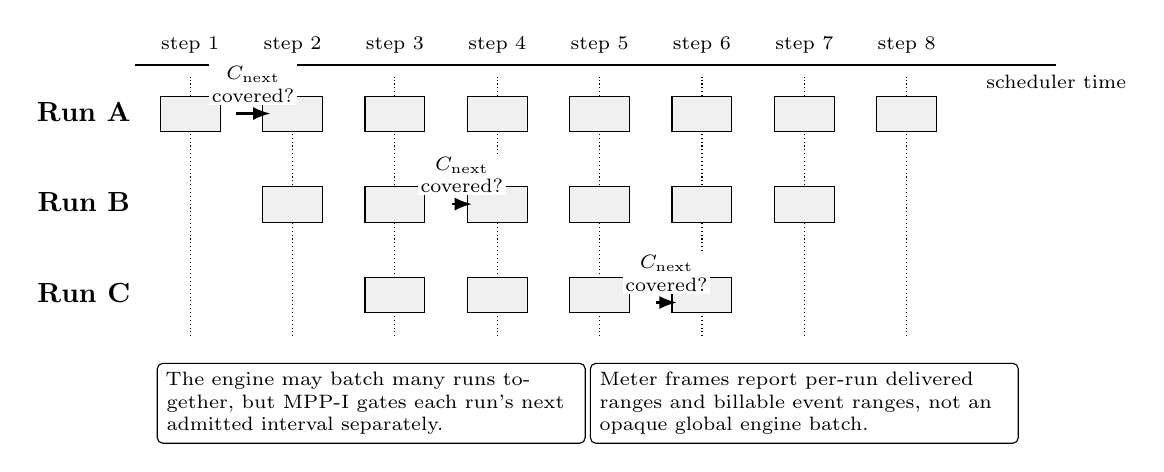
\begin{tikzpicture}[x=1cm,y=1cm, font=\scriptsize]
  \node[font=\bfseries] at (-0.65,2.4) {Run A};
  \node[font=\bfseries] at (-0.65,1.25) {Run B};
  \node[font=\bfseries] at (-0.65,0.1) {Run C};
  \draw[thick] (0,3.0) -- (11.7,3.0) node[below] {scheduler time};

  \foreach \x/\label in {0.7/step 1,2.0/step 2,3.3/step 3,4.6/step 4,5.9/step 5,7.2/step 6,8.5/step 7,9.8/step 8} {
    \draw[densely dotted] (\x,-0.45) -- (\x,2.85);
    \node[align=center] at (\x,3.25) {\label};
  }

  \foreach \x in {0.7,2.0,3.3,4.6,5.9,7.2,8.5,9.8}
    {\draw[fill=gray!12] (\x-0.38,2.15) rectangle +(0.76,0.45);}
  \foreach \x in {2.0,3.3,4.6,5.9,7.2,8.5}
    {\draw[fill=gray!12] (\x-0.38,1.0) rectangle +(0.76,0.45);}
  \foreach \x in {3.3,4.6,5.9,7.2}
    {\draw[fill=gray!12] (\x-0.38,-0.15) rectangle +(0.76,0.45);}

  \draw[payflow] (1.28,2.38) -- (1.72,2.38);
  \draw[payflow] (4.02,1.23) -- (4.28,1.23);
  \draw[payflow] (6.62,-0.02) -- (6.88,-0.02);
  \node[align=center, fill=white, inner sep=1pt] at (1.5,2.75) {\(C_{\mathrm{next}}\)\\covered?};
  \node[align=center, fill=white, inner sep=1pt] at (4.15,1.6) {\(C_{\mathrm{next}}\)\\covered?};
  \node[align=center, fill=white, inner sep=1pt] at (6.75,0.35) {\(C_{\mathrm{next}}\)\\covered?};

  \node[note, text width=5.2cm] at (3.0,-1.3)
    {The engine may batch many runs together, but \mppi{} gates each run's next admitted interval separately.};
  \node[note, text width=5.2cm] at (8.5,-1.3)
    {Meter frames report per-run delivered ranges and billable event ranges, not an opaque global engine batch.};
\end{tikzpicture}%
}
\caption{Continuous batching with per-run payment gates. A global engine batch is not the buyer-visible billing boundary; each run must have authorised headroom before its next admitted interval.}
\label{fig:continuous-batching-gates}
\end{figure}

The buffer is not a fee. It is a risk and latency control. It gives the provider enough authorised headroom to continue a bounded unit of inference without waiting for a payment message at every token.

Watermarks should be ordered in the same money-denominated unit and evaluated against the current disclosed metering boundary:

\[
L_t \geq D_t \geq H_t^{\mathrm{state}}
\]

The intended credit-state convention is a direct function of the applicable available amount at each disclosed boundary. Before admission it is evaluated against \(a_t\). Immediately after reserving a newly admitted interval it may be evaluated against \(a_t^{\mathrm{reserve}(j)}\) for telemetry and future-admission state. After a meter frame posts and an active bound is removed or reduced it is evaluated against \(a_t^{\mathrm{posted}}\). The post-reservation value does not retroactively reject the interval that was just admitted; it controls warning, drain, and later admission.

\[
\mathrm{credit\_state}(a_t)=
\begin{cases}
\text{\field{credit_ok}}, & a_t \geq L_t\\
\text{\field{low_credit}}, & L_t > a_t \geq D_t\\
\text{\field{draining}}, & D_t > a_t \geq H_t^{\mathrm{state}}\\
\text{\field{credit_stopped}}, & a_t < H_t^{\mathrm{state}}
\end{cases}
\]

Equality is intentionally kept in the higher-credit state so that implementations do not disagree at exact boundary values. Profiles that require distinct warning and drain intervals should set \(L_t > D_t > H_t^{\mathrm{state}}\). Profiles may set \(L_t = D_t\) or \(D_t = H_t^{\mathrm{state}}\), but then the adjacent state collapses: \(L_t = D_t\) gives no distinct \field{low_credit} interval, and \(D_t = H_t^{\mathrm{state}}\) gives no distinct \field{draining} interval. Jumps across multiple thresholds take the deepest matching state directly; an implementation should not be required to pass through \field{low_credit} before entering monetary \field{draining} or \field{credit_stopped}.

Acknowledgement lag is a separate delivery-lag state, not another meaning of \(D_t\). Optional warning thresholds use explicit enabled sets so omitted dimensions cannot accidentally trigger or suppress \field{ack_lag_low}. Let \(W_R\) mean the range warning threshold is enabled and \(W_E\) mean the exposure warning threshold is enabled:

\[
\begin{aligned}
\mathrm{ack\_warn}_t \iff
&(W_R \land R_{\mathrm{unacked},t} > R_{\mathrm{low}})\\
&\lor
(W_E \land E_{\mathrm{unacked},t} > E_{\mathrm{low}})
\end{aligned}
\]

\[
\mathrm{ack\_state}_t=
\begin{cases}
\text{\field{ack_lag_exceeded}}, &
\lnot \mathrm{ack\_lag\_ok}_t\\
\text{\field{ack_lag_low}}, &
\mathrm{ack\_lag\_ok}_t
\land
\mathrm{ack\_warn}_t\\
\text{\field{ack_ok}}, &
\mathrm{ack\_lag\_ok}_t
\land
\lnot \mathrm{ack\_warn}_t
\end{cases}
\]

Equality follows the same higher-state convention as monetary credit thresholds: equality at \(R_{\mathrm{low}}\) or \(E_{\mathrm{low}}\) does not trigger \field{ack_lag_low}, and equality at \(\bar{R}_{\mathrm{unacked}}\) or \(\bar{E}_{\mathrm{unacked}}\) remains \field{ack_lag_ok}.

If a profile does not define \(R_{\mathrm{low}}\), set \(W_R=\mathrm{false}\). If it does not define \(E_{\mathrm{low}}\), set \(W_E=\mathrm{false}\). If both warning dimensions are disabled, \field{ack_lag_low} is unreachable and the state moves directly from \field{ack_ok} to \field{ack_lag_exceeded}. Enabled warning thresholds must not exceed their corresponding stop thresholds. Top-ups recompute and may improve monetary credit state; sufficient top-ups restore \field{credit_ok}. \field{DeliveryAck}, transport backpressure, slower emission, or stopping at the disclosed delivery boundary recomputes or handles acknowledgement-lag state; sufficient acknowledgement restores \field{ack_ok}. If the next interval would exceed the quote's disclosed cost bound, the client's policy, monetary credit state, or acknowledgement-lag guard, the provider must quote again, request fresh authorisation or acknowledgement, apply the disclosed slow-consumer policy, or stop before execution enters that interval.

\textbf{Acknowledgement-lag stop.} If \field{ack_lag_exceeded} occurs while an output-producing interval is active, the provider must not treat the interval's planned boundary as automatically finishable. The profile must define an ack-lag stop boundary. Under the base acknowledged-billable profile, the provider closes the interval at the latest accepted \field{DeliveryAck} boundary, posts only the acknowledged billable amount to \field{cumulative_amount_due}, reports any delivered but unacknowledged range as provider-risk exposure, and treats generated but undelivered output as provider risk. The active interval's \field{meter_status} must become \field{posted} for the acknowledged portion and \field{reduced}, \field{released}, or \field{disputed} for the remaining active bound according to the profile. The provider then removes or reduces the affected \(C_i^{\max}\) from \(B_{\mathrm{active},t}\), emits the terminal or reduced \field{MeterFrame} and \field{Stop} where terminal, recomputes \(P_t\), \(B_{\mathrm{active},t}\), \field{credit_state}, and \field{ack_state}, and carries the stop boundary, delivered-but-unacknowledged range, and meter status into \field{FinalReceipt}. A weaker delivery-boundary profile may stop at a disclosed transport boundary, but it must state which unacknowledged output, if any, can become billable and how the receipt exposes that boundary.

Credit state and acknowledgement-lag state are not execution phases. \field{run_execution_state} is a high-level lifecycle state; prefill, decode, tool units, KV hold, multimodal work, reasoning-token intervals, and scheduler-admitted accelerator intervals belong in \field{active_admitted_intervals}. They may coexist, and each active interval is allowed only while the current credit state and acknowledgement-lag state permit the next disclosed boundary.

\begin{figure}[H]
\centering
\resizebox{\linewidth}{!}{%
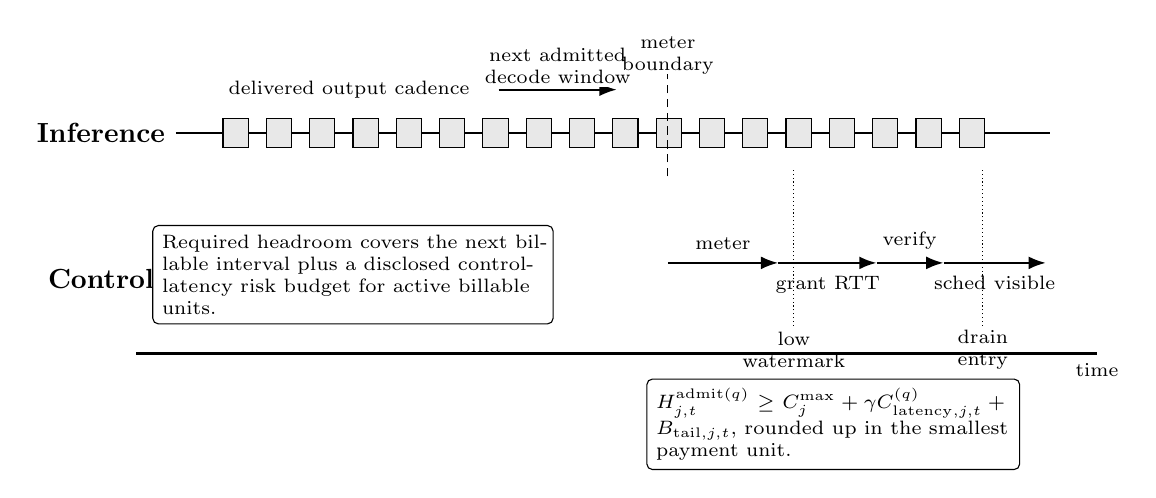
\begin{tikzpicture}[x=1cm,y=1cm, font=\scriptsize]
  \draw[thick] (0,0) -- (12.2,0) node[below] {time};
  \node[font=\bfseries] at (-0.45,2.8) {Inference};
  \node[font=\bfseries] at (-0.45,0.95) {Control};

  \draw[thick] (0.5,2.8) -- (11.6,2.8);
  \foreach \x in {1.1,1.65,2.2,2.75,3.3,3.85,4.4,4.95,5.5,6.05,6.6,7.15,7.7,8.25,8.8,9.35,9.9,10.45}
    {\draw[fill=gray!18] (\x,2.62) rectangle +(0.32,0.36);}
  \node[align=center] at (2.7,3.35) {delivered output cadence};
  \draw[flow] (4.6,3.35) -- (6.1,3.35);
  \node[align=center, fill=white, inner sep=1pt] at (5.35,3.65) {next admitted\\decode window};
  \draw[densely dashed] (6.75,2.25) -- (6.75,3.55);
  \node[align=center] at (6.75,3.78) {meter\\boundary};

  \draw[payflow] (6.75,1.15) -- (8.15,1.15);
  \node[above, fill=white, inner sep=1pt] at (7.45,1.28) {meter};
  \draw[payflow] (8.15,1.15) -- (9.4,1.15);
  \node[below, fill=white, inner sep=1pt] at (8.78,1.02) {grant RTT};
  \draw[payflow] (9.4,1.15) -- (10.25,1.15);
  \node[above, fill=white, inner sep=1pt] at (9.82,1.28) {verify};
  \draw[payflow] (10.25,1.15) -- (11.55,1.15);
  \node[below, fill=white, inner sep=1pt] at (10.9,1.02) {sched visible};

  \draw[densely dotted] (8.35,0.35) -- (8.35,2.35);
  \draw[densely dotted] (10.75,0.35) -- (10.75,2.35);
  \node[align=center] at (8.35,0.05) {low\\watermark};
  \node[align=center] at (10.75,0.05) {drain\\entry};

  \node[note, text width=4.85cm] at (2.75,1.0)
    {Required headroom covers the next billable interval plus a disclosed control-latency risk budget for active billable units.};
  \node[note, text width=4.5cm] at (8.85,-0.9)
    {\(H_{j,t}^{\mathrm{admit}(q)} \geq C_j^{\max} + \gamma C_{\mathrm{latency},j,t}^{(q)} + B_{\mathrm{tail},j,t}\), rounded up in the smallest payment unit.};
\end{tikzpicture}%
}
\caption{Admission headroom sizing under control-plane latency. In the base paper profile, admission headroom covers the candidate billable interval plus a disclosed quantile-based control-latency risk budget for active billable units while meter frames, grants, verification, and scheduler visibility propagate.}
\label{fig:mppi-headroom}
\end{figure}

\section{Protocol Objects}

The following objects are the minimum useful surface for an \mppi{} specification.

This remains paper-level shape, not a complete wire specification. Interoperable profiles must define protocol versioning, canonical serialisation, object type tags, signature suites, domain separation, asset identifiers, network identifiers, decimal and smallest unit rules, clock skew rules, problem codes, transport mappings, settlement method mappings, and dispute opening procedures.

Signed payment/control objects should bind private inference content by digest or hiding commitment rather than carrying raw prompt, raw output, or raw transcript material. For POST inference requests, a Payment HTTP body digest or equivalent canonical request digest can bind payment objects to the private HTTP request, but a deterministic digest is not by itself a content-private commitment for low entropy or guessable content. Payment plane privacy requires a salted or blinded, domain-separated hiding commitment profile for request, delivered output, and billable event commitments. Large quotes should be referenced by \field{quote_id} and \field{quote_hash} when they are too large for compact HTTP headers; the signed policy, grants, meter frames, and receipt then bind to the digest rather than copying the full quote through every message.

Digest fields name a canonical object body; they are not included in the byte string whose digest they name. A formal profile should define \field{InferenceQuoteBody} as the quote body excluding \field{quote_hash} and envelope metadata, then compute:

\[
\text{\field{quote_hash}} =
H(\mathrm{domain} \parallel \mathrm{canonical}(\text{\field{InferenceQuoteBody}}))
\]

\field{InferencePolicyBody} should be defined similarly, excluding \field{policy_hash} while still binding to \field{quote_hash}. Profiles may carry these hashes in an envelope, challenge parameter, reference object, or object row, but the digest field is excluded from its own digest target.

The object table below is a paper-level inventory, not a self-hashing schema. Its ``fields or bindings to specify'' column may name body fields, envelope or reference fields, and derived digest fields in the same row. A formal wire profile should split each signed object into an explicit body, envelope/reference fields, and derived digest fields, then state exactly which bytes each digest and signature covers. For auditability, the formal specification should also split this inventory into identity and binding fields, pricing and gate fields, delivery fields, evidence fields, and settlement fields.

{\footnotesize
\begin{longtable}{@{}>{\raggedright\arraybackslash}p{0.17\linewidth} >{\bfseries\raggedright\arraybackslash}p{0.19\linewidth} >{\raggedright\arraybackslash}p{0.58\linewidth}@{}}
\caption{Proposed \mppi{} object inventory by field group}\label{tab:mppi-objects}\\
\toprule
\textbf{Object} & \textbf{Group} & \textbf{Purpose, fields, or bindings to specify} \\
\midrule
\endfirsthead
\toprule
\textbf{Object} & \textbf{Group} & \textbf{Purpose, fields, or bindings to specify} \\
\midrule
\endhead
\field{InferenceQuote} & Purpose & Provider's machine-readable offer. \\
 & Identity and binding & Payment challenge ID, proposed \field{run_id} or provider run nonce for deriving it, quote ID, quote hash, provider ID, request commitment rule. \\
 & Inference description & Inference target or model ID, tokenizer ID and version, chat template or canonical serialisation profile, special-token policy, tool or function schema hash, multimodal preprocessing profile where used, context-window and truncation policy, cache-hit class. \\
 & Pricing and admission & Exact unit prices or price schedule hash, quote line item identifiers, exact or conservative input/prefill token count, \field{required_initial_credit}, \field{minimum_execution_buffer}, low and drain-entry watermarks, metering boundary policy, meter cadence, maximum admitted interval, \(C_{\mathrm{next}}^{\max}\) bound or cap semantics, \(q\), \(\gamma\), \field{admission_latency_profile}, \field{finish_latency_profile}, \field{admission_tail_margin}, \field{finish_tail_margin}, \field{tail_overrun_policy}, deterministic maxima where used, shared-alias rule for latency and tail fields, rounding rule. \\
 & Delivery and payment & Delivery semantics profile, acknowledgement cadence, slow-consumer policy, metadata profile, accepted payment methods and settlement destinations, max context/output, queue timeout, expiry. \\
\midrule
\field{InferencePolicy} & Purpose & Client's signed constraints. \\
 & Identity and binding & Payment challenge ID, \field{run_id} or one-to-one policy/run binding, quote ID, quote hash, policy ID, policy hash, request commitment, provider ID. \\
 & Inference constraints & Inference target or model ID, tokenizer ID and version, serialisation profile, delivery semantics profile, acknowledgement cadence, slow-consumer policy, metadata profile, max context/output, max output tokens, allowed tools/modalities, allowed cache-hit class, provider-observed billable unit policy, optional explicitly priced KV hold or accelerator-time policy. \\
 & Spend and payment & Exact unit prices or price schedule hash, accepted payment method, settlement destination, \field{claim_reference_hash} or profile-defined claim-reference commitment/null value, max total, expiry, payer, delegated signer. \\
\midrule
\field{RunPaymentState} & Purpose & Accounting and admission state local to the provider for a run, unless a profile exposes it. \\
 & Identity and lifecycle & Globally unique unguessable \field{run_id}, payment challenge ID, quote ID and hash, policy ID and hash, request commitment, \field{claim_reference_hash} or profile-defined claim-reference commitment/null value, execution lifecycle state, queue state, scheduler admission state, payment-state version. \\
 & Credit and gate state & Credit state, acknowledgement-lag state, cumulative authorised amount, valid authorised amount, computed \(A_t^{\mathrm{gate}}\), local \field{posted_cumulative_amount_due} with wire alias \field{cumulative_amount_due}, available amount for new admission, interval-specific finish amount where needed, required headroom, \field{minimum_execution_buffer}, low watermark, drain-entry watermark. \\
 & Active intervals & Active admitted interval set with quote line item, maximum cost, grant-validity or claimability snapshot, total active admitted bound, metering boundary policy. \\
 & Sequence cursors & Latest accepted grant sequence, latest accepted meter frame sequence, latest generated sequence, latest emitted sequence, latest transport-flushed sequence where used, latest signed delivered sequence, latest accepted \field{DeliveryAck} sequence and hash where used, latest billable output sequence. \\
 & Expiry and release & Expiry, reservation release state, payment method or settlement path. \\
\midrule
\field{DeliveryAck} & Purpose & Signed acknowledgement of delivered output used as a billability boundary. \\
 & Identity and authority & DeliveryAck ID, DeliveryAck sequence or control sequence, \field{run_id}, payment challenge ID, quote hash, policy hash, acknowledgement authority role and signer key ID authorised by the quote and policy. \\
 & Delivery boundary & Acknowledged delivered sequence range or cumulative latest acknowledged delivered sequence, delivered-unit commitment root under the content-private commitment profile. \\
 & References and signature & Latest accepted \field{MeterFrame} sequence and hash or profile-defined genesis meter-frame reference, optional latest accepted grant sequence and hash, optional previous DeliveryAck hash, timestamp or validity window, metadata placement profile, signature. \\
\midrule
\field{CreditGrant} & Purpose & Cumulative authorisation to spend up to a stated cap. \\
 & Identity and binding & Grant ID, grant sequence, \field{run_id}, payment challenge ID, policy ID, policy hash, quote hash, request commitment, provider ID, \field{claim_reference_hash} or profile-defined claim-reference commitment/null value. \\
 & Causal references & Acked meter frame sequence, grant issuer replay-window or acceptance-window rule where used, latest accepted \field{DeliveryAck} sequence or hash when output billing uses \field{acknowledged_delivered_output}, acknowledged delivered sequence or range. \\
 & Authorisation and validity & Cumulative authorised amount, valid from and valid until timestamps, payment method or settlement path, optional previous grant hash, payer or facilitator signature. \\
\midrule
\field{MeterFrame} & Purpose & Provider-signed cumulative usage update. \\
 & Identity and sequence & \field{run_id}, payment challenge ID, quote ID and hash, policy ID and hash, request commitment, provider ID, sequence, optional previous meter frame hash. \\
 & Delivery and billing & Output delivered-sequence range, \field{DeliveryAck} reference when output amount due uses acknowledged delivery, separate billable-event range where non-output units are charged, billing boundary. \\
 & Usage counters & Input/cached/output token counters, accepted speculative-token counters where used, reasoning token counters, tool units, multimodal units, explicitly quoted KV hold or accelerator-time units. \\
 & Evidence and amount due & Non-output evidence profile and evidence root where used, \field{cumulative_amount_due}, content-private commitment/root over delivered units and billable events, timestamp policy, provider signature. \\
\midrule
\field{FinalReceipt} & Purpose & Final provider signed settlement and usage record. \\
 & Identity and binding & \field{run_id}, payment challenge ID, quote ID and hash, policy ID and hash, request commitment, provider ID, payment method or settlement path, \field{claim_reference_hash} or profile-defined claim-reference commitment/null value, HTTP \field{Payment-Receipt} carriage mode where used. \\
 & Delivery, usage, and evidence & Delivery semantics profile, terminal \field{DeliveryAck} sequence and hash where used, \field{delivery_commitment_profile}, \field{delivered_unit_commitment_root}, \field{billable_event_commitment_root} where used, \field{non_output_evidence_root}, \field{evidence_profile_id}, terminal evidence-record root or hash where used, inference target or model ID, tokenizer ID and version, serialisation profile, \field{usage_totals}, \field{timing}, \field{terminal_meter_frame_sequence} and \field{terminal_meter_frame_hash}, \field{latest_grant_sequence} and \field{latest_grant_hash}, \texttt{latest\_acknowledged\_delivered\_}\allowbreak\texttt{sequence\_or\_range}, and \texttt{terminal\_or\_}\allowbreak\texttt{cancellation\_boundary}. \\
 & Settlement cap and target & \field{final_metered_amount_due}, \field{settlement_cap}, \field{run_claimable_limit}, \field{settlement_target_amount}, \field{settlement_attempted_amount} where used, \field{settlement_cap_cause}, \field{authorisation_shortfall_reason} where applicable, \field{unused_authorisation_amount}, \field{released_run_claimable_amount} or reservation release state. \\
 & Finality and refund state & \field{settled_gross_amount} and \field{refunded_amount} where used, \field{settled_amount}, \field{uncollected_collectible_amount}, \field{over_cap_metered_amount}, \field{over_cap_cause}, \field{over_settled_amount}, \field{refund_adjustment_amount} where used, \field{refund_due_amount}, \field{refund_status}, \field{refund_deadline} where used, \field{settlement_reference}, \field{settlement_status}, \field{settlement_finality}, \field{terminal_reason}, \field{idempotency_key}, provider signature, optional client acknowledgement. \\
\bottomrule
\end{longtable}
}

\field{minimum_execution_buffer} is the canonical name for the money-denominated minimum buffer used in the headroom rule. If an early profile or draft field uses \field{minimum_buffer}, it should be treated as an alias for \field{minimum_execution_buffer} or renamed before interoperability testing.

The base profile should establish \field{run_id} before policy signing. The simplest construction is for the provider to place an unguessable \field{run_id} directly in the executable quote. A nonce-derived construction is also workable, but the dependency order must be explicit:

\begin{enumerate}
  \item The provider quote body contains \field{payment_challenge_id}, \field{provider_run_nonce}, quote ID, provider ID, inference target, request-commitment rule, price schedule, and expiry.
  \item The quote hash is computed over \field{InferenceQuoteBody}, excluding \field{quote_hash} and envelope metadata.
  \item The client or wallet chooses \field{policy_id} and computes the content-private request commitment under the quote's commitment rule.
  \item Both sides derive \field{run_id} from a domain-separated hash over \field{payment_challenge_id}, \field{quote_hash}, \field{policy_id}, \field{provider_run_nonce}, and the request commitment.
  \item \field{InferencePolicyBody} includes the derived \field{run_id}, \field{policy_id}, \field{quote_hash}, request commitment, provider ID, payment method, settlement destination, max spend, allowed units, and expiry. \field{policy_hash} is then computed over that policy body, excluding \field{policy_hash} itself.
  \item The provider rejects any \field{CreditGrant}, \field{DeliveryAck}, \field{MeterFrame}, or \field{FinalReceipt} whose \field{run_id} does not match the selected construction.
\end{enumerate}

In either construction, \field{InferencePolicy}, the genesis \field{CreditGrant}, \field{DeliveryAck}, \field{MeterFrame}, and \field{FinalReceipt} must bind the same \field{run_id}. The provider should reject a second \field{run_id} for the same quote, policy, and request commitment. Alternative profiles may allow a wallet or facilitator to create \field{run_id}, but only if it is created before policy signing and explicitly provider-bound before the genesis grant is accepted.

The initial \field{CreditGrant} is a genesis grant because it is issued before any \field{MeterFrame} or \field{DeliveryAck} exists. Each profile must define a genesis payment-state vector for that grant. The genesis vector should bind the \field{run_id}, quote, policy, request commitment, provider, claim reference or profile-defined claim-reference convention, and cumulative authorised amount, while setting meter and acknowledgement references to profile-defined genesis values such as \field{acked_meter_frame_sequence = 0}, \field{genesis_meter_hash}, null \field{DeliveryAck} sequence or hash, and an empty acknowledged delivered range. The first \field{DeliveryAck} should use the same profile-defined genesis meter-frame reference until a provider \field{MeterFrame} exists; later acknowledgements should bind the latest accepted \field{MeterFrame} sequence and hash when the profile uses that reference. Later \field{CreditGrant} messages should reference a causally accepted \field{MeterFrame} and, where acknowledged-output billing is used, the latest accepted \field{DeliveryAck} visible to the grant issuer under the profile's acceptance rule.

A formal profile should define grant acceptance under meter-frame concurrency. The grant issuer's \field{acked_meter_frame_sequence} must be non-decreasing for that issuer and run. The provider may accept a grant that references meter frame \(N\) after it has emitted \(N+1\), provided \(N\) is within the disclosed acceptance window, is not below the provider's minimum required acknowledgement sequence for new admission, and the grant sequence, cumulative authorised amount, validity interval, policy binding, and method claimability are all acceptable. The provider should reject a grant that decreases grant sequence, cumulative authorised amount, or acknowledged meter-frame sequence; references a meter frame below the accepted replay window; is stale after terminal settlement; or is not bound to the current run, policy, payment method, and claim state. Reconnect handling should use the same cumulative monotonic rules so delayed grants can top up only the latest valid run state and cannot roll metering or settlement backwards.

Under an acknowledged-billable profile, \field{latest_billable_output_sequence} is the output boundary that may advance output amount due. Generated, emitted, transport-flushed, and signed-delivered sequences may be useful for reconciliation and slow-consumer handling, but they do not by themselves make output billable.

{\footnotesize
\emph{Table~\ref{tab:mppi-binding-chain} is a proposed future-profile binding checklist. It inherits the required object content in Table~\ref{tab:mppi-objects}; a formal profile must state whether each field is carried directly, covered by a referenced body hash, or derived from a domain-separated commitment.}
\vspace{0.5em}

\begin{longtable}{@{}>{\bfseries\raggedright\arraybackslash}p{0.21\linewidth} >{\raggedright\arraybackslash}p{0.50\linewidth} >{\raggedright\arraybackslash}p{0.23\linewidth}@{}}
\caption{Canonical signed-object bindings}
\label{tab:mppi-binding-chain}\\
\toprule
Signed object body & Future profile should include or hash & Attack prevented \\
\midrule
\endfirsthead
\toprule
Signed object body & Future profile should include or hash & Attack prevented \\
\midrule
\endhead
\field{InferenceQuoteBody} & \field{payment_challenge_id}, \field{provider_id}, proposed \field{run_id} or provider run nonce, \field{quote_id}, inference target, serialisation and tokenisation profile, price schedule, delivery and acknowledgement policy, metering policy, expiry. & Reusing a quote under a different payment challenge or provider offer. \\
\field{InferencePolicyBody} & \field{payment_challenge_id}, \field{run_id} or one-to-one policy/run binding, \field{quote_id}, \field{quote_hash}, \field{policy_id}, \field{request_commitment}, \field{provider_id}, inference target or model ID, tokenizer and serialisation profile, payment method, settlement destination, \field{claim_reference_hash} or profile-defined null convention, max spend, allowed units, expiry. & Separating the private inference request from the signed spend policy. \\
\field{DeliveryAckBody} & \field{payment_challenge_id}, \field{run_id}, \field{quote_hash}, \field{policy_hash}, \field{provider_id} and \field{request_commitment} directly or through the covered policy body, acknowledgement authority role, signer key ID, acknowledged delivered range, delivered-unit commitment, latest accepted \field{MeterFrame} sequence and hash or profile-defined genesis meter-frame reference, optional latest accepted grant reference, sequence, validity window. & Charging output outside the authorised delivery acknowledgement boundary. \\
\field{CreditGrantBody} & \field{payment_challenge_id}, \field{run_id}, \field{policy_id}, \field{policy_hash}, \field{quote_hash}, \field{request_commitment}, \field{provider_id}, payment method or settlement path, \field{claim_reference_hash} or profile-defined claim-reference commitment/null value, grant sequence, latest accepted meter-frame sequence or profile-defined genesis value, latest accepted \field{DeliveryAck} or profile-defined genesis value where used, acknowledged delivered range where used, cumulative authorised amount, validity interval, signer. & Replaying grants, rolling back authorisation, or using one claimable funding state across unrelated runs. \\
\field{MeterFrameBody} & \field{payment_challenge_id}, \field{run_id}, \field{quote_id}, \field{quote_hash}, \field{policy_id}, \field{policy_hash}, \field{request_commitment}, \field{provider_id}, payment method or settlement path directly or through the covered policy body, sequence, previous meter-frame hash where used, delivered range, billable range, \field{DeliveryAck} reference where used, billable-event root, non-output evidence root where used, cumulative amount due, timestamp policy. & Reordering usage, overcounting output, or mixing acknowledged billable usage with provisional delivery. \\
\field{FinalReceiptBody} & \field{run_id}, \field{payment_challenge_id}, \field{quote_id}, \field{quote_hash}, \field{policy_id}, \field{policy_hash}, \field{request_commitment}, \field{provider_id}, \field{payment_method} or \field{settlement_path}, \field{claim_reference_hash} or profile-defined claim-reference commitment/null value, receipt carriage or reference method, delivery semantics profile, terminal meter-frame sequence and hash, latest grant sequence and hash, terminal \field{DeliveryAck} where used, delivery, billable-event, and non-output evidence commitments, usage totals, settlement reference, settlement status and finality, \field{cumulative_amount_due}, \field{final_metered_amount_due}, \field{settlement_cap}, \field{run_claimable_limit}, \field{settlement_target_amount}, \field{settlement_attempted_amount} where used, \field{settled_gross_amount} and \field{refunded_amount} where used, \field{settled_amount}, \field{uncollected_collectible_amount}, \field{over_cap_metered_amount}, \field{over_cap_cause} where used, \field{over_settled_amount}, \field{refund_adjustment_amount} where used, \field{refund_due_amount}, \field{refund_status}, and \field{refund_deadline} where used, terminal reason, idempotency key. & Duplicating settlement or issuing a receipt that cannot be reconciled to the run state. \\
\bottomrule
\end{longtable}
}

In Table~\ref{tab:mppi-binding-chain}, the direction is explicit: the named signed object body includes or hashes the listed fields. If a row relies on \field{quote_hash}, \field{policy_hash}, or another digest rather than repeating a field directly, the formal profile must define the covered body and show that the digest commits to that field. Profiles may add fields, but they should not remove the run, quote, policy, delivery, grant, meter, claim, provider, request, payment-method, or settlement bindings that make replay and substitution attacks detectable.

A final receipt is valid only if these direct bindings and the referenced terminal objects validate against the same run, quote, policy, request commitment, provider, payment method, and claim state. A verifier should reject a receipt that presents a valid settlement reference but cannot reconcile the terminal meter frame, latest grant, terminal \field{DeliveryAck} where used, and final usage totals to the same signed lifecycle. If the HTTP \field{Payment-Receipt} header carries only a compact receipt reference, the referenced signed body must be digest-bound to the challenge, run, policy, meter frames, and settlement reference.

\field{claim_reference_hash} is payment-method neutral. A direct profile may map it to an escrow, allowance nonce, voucher channel state, or channel-state root. A facilitated profile may map it to a facilitator reservation or credit-assurance object. If a payment method does not expose a separate claim reference, the method profile should define a signed null value or equivalent claim-reference commitment under the payment-method mapping and profile identifier. A null claim-reference convention is valid only when the method profile separately defines provider-verifiable, run-scoped claimability and computes \field{run_claimable_limit}; it must not represent absent or unverifiable funding state. The requirement is that a run-bound grant is tied not only to the run and policy, but also to the claimable funding state, or explicit method-level claim convention, that makes the grant economically enforceable.

Credit grants should be cumulative, not incremental. A cumulative grant is easier to verify, easier to settle, and safer under retries. If the latest valid grant authorises 50 cents and an earlier grant authorised 30 cents, the \$0.50 grant is a settlement cap for that run, not the cumulative metered amount due. A provider should accept only strictly increasing grant sequences, non-decreasing cumulative authorised amounts within policy, a \field{run_id} that is globally unique and unguessable for the chosen profile, and grants whose acknowledged meter frame sequence is acceptable under the causal replay-window rule. This prevents a valid old grant from rolling the run back to a lower authorisation after reconnect or duplicate delivery.

Final settlement should separate the collection cap, the intended collection target, gross value movement where it exists, refunds where they exist, and the amount finally retained by the provider. The cap is constrained by the latest valid cumulative authorisation, by the client policy, and by the run-scoped amount actually claimable or retainable under the selected payment method:

\[
\begin{aligned}
\mathrm{settlement\_cap} =
\min(&\mathrm{latest\_cumulative\_authorised\_amount},\\
     &\mathrm{policy\_max\_total},\\
     &\mathrm{run\_claimable\_limit})
\end{aligned}
\]

Here \field{run_claimable_limit} is the method-profile-computed maximum amount verifiably claimable or retainable for this run. It may be backed by escrow, an allowance nonce, channel state, a voucher state root, a facilitator reservation, a prior push payment, or another atomic method convention. A separate \field{claimable_reserved_amount} can exist inside one method profile, but it is not the generic settlement-cap term.

\[
\mathrm{settlement\_target\_amount} =
\min(\mathrm{final\_metered\_amount\_due}, \mathrm{settlement\_cap})
\]

\[
\mathrm{over\_cap\_metered\_amount} =
\max(0,\mathrm{final\_metered\_amount\_due} - \mathrm{settlement\_cap})
\]

When gross/refund fields are used:

\[
\begin{aligned}
0 &\leq \mathrm{settled\_gross\_amount}\\
0 &\leq \mathrm{refunded\_amount}
\leq \mathrm{settled\_gross\_amount}\\
\mathrm{settled\_amount} &=
\mathrm{settled\_gross\_amount} - \mathrm{refunded\_amount}
\end{aligned}
\]

\[
\mathrm{over\_settled\_amount} =
\max(0,\mathrm{settled\_amount} - \mathrm{settlement\_target\_amount})
\]

\[
\mathrm{refund\_due\_amount} =
\mathrm{over\_settled\_amount}
+ \mathrm{refund\_adjustment\_amount}
\]

\[
\mathrm{refund\_adjustment\_amount} \geq 0
\]

\[
\mathrm{uncollected\_collectible\_amount} =
\max(0,\mathrm{settlement\_target\_amount} - \mathrm{settled\_amount})
\]

\begin{table}[H]
\centering
\caption{Canonical settlement fields}
\label{tab:canonical-settlement-fields}
\footnotesize
\begin{tabularx}{\linewidth}{>{\bfseries\raggedright\arraybackslash}p{0.31\linewidth} >{\raggedright\arraybackslash}p{0.24\linewidth} >{\raggedright\arraybackslash}X}
\toprule
Canonical field & Human label & Meaning \\
\midrule
\field{settlement_target_amount} & Settlement target & Amount the provider is entitled to try to collect, equal to final metered amount due capped by \field{settlement_cap}. \\
\field{settlement_attempted_amount} & Settlement attempt & Amount submitted in the current idempotent settlement attempt, where used. It is not summed across retries and is not the final retained amount. \\
\field{settled_amount} & Net retained settlement & Status-conditioned net provider-retained amount: current net retained amount while settlement is non-final, and final provider-retained amount once \field{settlement_status} is final. \\
\field{uncollected_collectible_amount} & Collectible shortfall & Collectible amount within the settlement target that was not finally retained. \\
\field{over_cap_metered_amount} & Over-cap metered amount & Metered amount above the settlement cap. It is not collectible under the current run authorisation. \\
\field{settlement_cap_cause} & Cap cause & Binding cap constraint when \field{settlement_cap} is below \field{final_metered_amount_due}; omitted, null, or \field{none} for normal under-cap settlement. \\
\field{authorisation_shortfall_reason} & Shortfall reason & Optional reason why usable authorisation or claimability did not cover final metered amount due before stop. This is diagnostic; it is not a cap formula. \\
\field{unused_authorisation_amount} & Unused authorisation & Latest accepted buyer authorisation not consumed by \field{settlement_target_amount}; this is buyer permission, not necessarily unused collectible cap. \\
\field{released_run_claimable_amount} & Released claimability & Method-profile amount of run-scoped reservation or claimability released after settlement, refund, or finality handling. Omitted or null when the method has no reservation/release concept. \\
\field{over_cap_cause} & Over-cap cause & Reason metered usage exceeded the cap, if it did. This is separate from the cap constraint. \\
\field{over_settled_amount} & Over-settlement & Non-final value retained above the settlement target before refund finality. \\
\field{refund_adjustment_amount} & Refund adjustment & Optional non-negative method-specific amount added to the refund due amount. The base profile sets it to zero. \\
\field{refund_due_amount} & Refund due & Amount that must be refunded or released when a non-final settlement has retained too much value. \\
\bottomrule
\end{tabularx}
\end{table}

\textbf{Derived receipt fields.} Let \(U_{\mathrm{auth}}\) denote \field{unused_authorisation_amount}, \(L_{\mathrm{auth}}\) denote \field{latest_cumulative_authorised_amount}, and \(S_{\mathrm{target}}\) denote \field{settlement_target_amount}. \field{unused_authorisation_amount} means unused buyer permission:

\[
U_{\mathrm{auth}} = \max(0,L_{\mathrm{auth}}-S_{\mathrm{target}})
\]

It is intentionally different from unused collectible cap. Let \(U_{\mathrm{cap}}\) denote an optional profile-specific unused collectible cap amount, and \(S_{\mathrm{cap}}\) denote \field{settlement_cap}:

\[
U_{\mathrm{cap}} = \max(0,S_{\mathrm{cap}}-S_{\mathrm{target}})
\]

A profile that needs to expose unused collectible cap should name that field separately rather than overloading \field{unused_authorisation_amount}. \field{released_run_claimable_amount} is method-profile specific. Let \(R_{\mathrm{release}}\) denote \field{released_run_claimable_amount} and \(R_{\mathrm{claim}}\) denote \field{run_claimable_limit}. For escrow, reservation, allowance, or voucher methods with explicit run-scoped release, a final normal receipt may set:

\[
R_{\mathrm{release}} = \max(0,R_{\mathrm{claim}}-S_{\mathrm{target}})
\]

If settlement, refund, reversal, dispute, or finality handling is not final, the receipt should carry a reservation release state such as \field{not_started}, \field{partial}, \field{pending_finality}, \field{released}, or \field{disputed}, and may report only the amount actually released under the selected method. Direct payment methods with no reusable reservation may omit \field{released_run_claimable_amount} or set it to a profile-defined null value.

\field{authorisation_shortfall_reason} is present only when \field{final_metered_amount_due} exceeds \field{settlement_cap}, or when the terminal reason is credit exhaustion caused by unavailable usable authorisation or claimability. It should explain the operational reason for the shortfall, such as \field{topup_missing}, \field{topup_invalid}, \field{grant_expired}, \field{policy_limit_reached}, \field{run_claimability_limit}, or \field{facilitator_reservation_unavailable}. It does not replace \field{settlement_cap_cause}, which identifies the binding cap constraint, or \field{over_cap_cause}, which explains why metered usage exceeded the cap.

Here \field{settled_amount} is status-conditioned. While settlement is non-final, it means the current net provider-retained amount visible under the selected payment method. Once \field{settlement_status} is \field{final}, it means the final provider-retained amount under that method's finality rule. \field{FinalReceipt} is the final run receipt, but settlement finality is status-conditioned. If \field{settlement_status} is \field{final}, the receipt must satisfy:

\[
\begin{aligned}
0 &\leq
\mathrm{settled\_amount}
\leq
\mathrm{settlement\_target\_amount},\\
\mathrm{over\_settled\_amount} &= 0,\quad
\mathrm{refund\_due\_amount}=0
\end{aligned}
\]

A positive \field{over_settled_amount} is therefore not valid in a settlement-final receipt. It is valid only in an explicitly non-final settlement status, such as \field{pending_finality}, \field{pending_refund}, \field{refund_due}, \field{refunding}, \field{disputed}, or \field{invalid}, as defined by the selected method profile. In those states the receipt must carry \field{refund_due_amount}, refund status, refund deadline or finality rule where applicable, and the settlement reference needed to reconcile value movement. In the base profile, \field{refund_adjustment_amount}=0 and \field{refund_due_amount} equals \field{over_settled_amount}. If a method profile permits a larger refund-due value, it must name the extra non-negative component and state whether it represents fees, release delays, disputed value, or another method-specific rule. Historical gross over-collection can still be visible through \field{settled_gross_amount} and \field{refunded_amount}; the final retained amount cannot exceed \field{settlement_target_amount} once refund finality is reached.

For methods with no gross push or refund, \field{settled_amount} can be reported directly and the gross/refund fields may be omitted. For methods where value is pushed, prepaid, escrowed, reserved, partially settled, or refunded, the receipt should also report \field{settled_gross_amount} and \field{refunded_amount}, with \field{settled_amount} computed as current net retained amount until finality and final net retained amount after refund finality. \field{settlement_attempted_amount}, where present, is scoped to the current idempotent settlement attempt or settlement reference; retries should reuse the idempotency key or issue a new attempt record rather than summing attempts into this field. The final receipt should use the canonical fields in Table~\ref{tab:canonical-settlement-fields}. This distinction matters because cumulative authorisation is permission to collect up to a cap; a method claim is the funding state that makes the cap enforceable; \field{settlement_target_amount} is the amount the provider is entitled to try to collect; \field{settlement_attempted_amount} is attempted movement for one settlement attempt; \field{settled_amount} is status-conditioned net retained value; \field{over_cap_metered_amount} is metered value outside the settlement cap, not a collectible shortfall; and \field{over_settled_amount} is non-final value retained above the settlement target before refund finality. \field{settlement_cap_cause} should be omitted, null, or set to \field{none} for normal under-cap settlement. When \field{settlement_cap} is below \field{final_metered_amount_due}, \field{settlement_cap_cause} should identify only the binding cap constraint using a profile enum such as \field{authorisation}, \field{policy_max_total}, or \field{run_claimable_limit}. \field{over_cap_cause} should separately describe why usage exceeded the cap, with values such as \field{provider_overrun}, \field{client_policy_stop}, \field{ack_lag_stop}, \field{latency_tail_overrun}, or \field{cancel_boundary}. Settlement failure, timeout, reversal, pending finality, refund due, and retry state should be represented by \field{settlement_status} and finality fields, not by \field{settlement_cap_cause}. These states should not be collapsed into one ``unused amount'' field.

Meter frames should also be cumulative. This makes omission and replay easier to detect. A client or facilitator can reject frames with nonmonotonic sequence numbers, unexpected \field{run_id} values, unexpected policy IDs, or amount changes inconsistent with the quote. Each meter frame should state the billing boundary used for its output component. Output usage should be represented as an output delivered-sequence range; non-output usage should be represented as a separate billable-event range with event type, admitted interval, meter evidence, and quoted pricing reference.

Non-output billable-event records should carry \field{billable_unit_type}, admitted interval, pricing reference, meter evidence hash or root, evidence profile ID, and an evidence reference such as \field{tool_receipt_hash}, provider-signed assertion hash, audit log reference, attestation reference, or dispute-opening rule. \field{MeterFrame} and \field{FinalReceipt} should bind the terminal hash or root over these evidence records, not only aggregate counters.

Commitment fields need a content-private commitment profile. The exact construction belongs in the technical specification, but the paper-level rule is clear: the payment/control plane may bind meter frames and receipts to delivered units and billable events, but it must not reveal raw prompt, raw output, or raw transcript. The final receipt should distinguish delivered output commitments from billable event commitments so that usage totals and the canonical settlement fields in Table~\ref{tab:canonical-settlement-fields} can be reconciled without exposing inference content.

Content privacy does not remove metadata risk. A profile should classify payment/control fields as \field{header_safe}, \field{signed_body_only}, \field{encrypted_body_only}, or \field{settlement_private}. Headers should carry only compact identifiers, hashes, nonces, version fields, and method hints needed for routing or authentication. Request commitments, meter evidence, delivery commitments, settlement details, and receipt bodies should be signed bodies or encrypted bodies when the selected transport allows it. Infrastructure logs and intermediaries should not store raw prompt, raw output, raw transcript, unnecessary payer/provider linkage, or unnecessary settlement linkage. Settlement references should be per-run unlinkable where the selected payment method permits it. The privacy claim is therefore content privacy under the selected commitment and transport profile, plus explicit metadata minimisation, not blanket privacy.

\section{Initial Protocol Flow}

The initial protocol flow should start conservatively.

\begin{table}[H]
\centering
\begin{tabularx}{0.96\linewidth}{>{\bfseries\raggedright\arraybackslash}p{0.08\linewidth} >{\raggedright\arraybackslash}X}
1 & Client sends a private inference request to a provider endpoint. \\
2 & Provider serialises and tokenises the request, or computes a conservative bound, without starting serving-engine execution. \\
3 & Provider returns an MPP \field{402} challenge carrying or referencing an \field{InferenceQuote} bound by digest: \field{run_id} or provider run nonce, inference target, tokenizer version, serialisation profile, unit prices, exact or conservative prefill bound, recommended reservation, required initial credit, watermarks, metering boundary policy, expiry, and accepted payment methods. \\
4 & Client signs an \field{InferencePolicy}: quote binding, \field{run_id}, request commitment, max total, max output, max unit prices, expiry, payment method, settlement destination, allowed billable units, and allowed cache-hit class. \\
5 & Grant issuer reserves or locks claimable funds for the \field{run_id}. \\
6 & Grant issuer sends an initial \field{CreditGrant} covering \field{required_initial_credit}: exact or conservatively bounded prefill plus first decode headroom, using the profile-defined genesis values for meter and delivery-acknowledgement references. \\
7 & Provider verifies the grant, records the payment-state version, and may place the run in a queue. \\
8 & Before scheduler admission, the provider revalidates the latest grant sequence and required headroom. \\
9 & Provider admits prefill and then per-run decode intervals only while \(\mathrm{may\_admit\_new\_interval}_{j,t}\) holds for each newly admitted interval. Already admitted bounded intervals may finish only while \(\mathrm{may\_finish\_interval}_{i,t}\) holds for each interval. \\
10 & Provider streams output on the inference plane under a signed delivered sequence. \\
11 & The authorised acknowledgement role sends \field{DeliveryAck} messages for delivered ranges under the selected acknowledgement cadence. \\
12 & Provider emits signed \field{MeterFrame} messages on the payment/control plane. In the acknowledged-billable profile, output amount due advances only through the latest accepted \field{DeliveryAck}; any delivered but unacknowledged range is separate from billable output. \\
13 & Grant issuer sends top-up \field{CreditGrant} messages before available amount drops below the money-denominated drain-entry watermark; the authorised acknowledgement role sends \field{DeliveryAck} messages before acknowledgement lag reaches the disclosed stop threshold. \\
14 & If credit runs low, provider emits \field{low_credit}; if the drain-entry watermark is crossed, provider emits \field{draining}, admits no new billable interval, and stops at the disclosed metering boundary unless a valid top-up restores admission. If acknowledgement lag exceeds the disclosed threshold, provider emits \field{ack_lag_exceeded} and applies the slow-consumer policy. \\
15 & Provider settles the cumulative metered amount due, capped by the latest valid cumulative grant, policy maximum, and run claimable limit, then emits a \field{FinalReceipt}. \\
\end{tabularx}
\caption{A minimal \mppi{} inference run}
\label{tab:minimal-mppi-run}
\end{table}

The \field{grant_issuer} role is selected by the payment profile. In direct mode it is the client or inference wallet. In facilitated mode it is the facilitator or credit-assurance service named by the profile. The provider verifies the issuer role, grant signature, grant sequence, \field{run_id}, quote and policy binding, \field{claim_reference_hash} or profile-defined claim-reference commitment/null value, and claimability or reservation state before accepting a grant. In direct mode the provider should accept a grant without contacting a facilitator only when the selected payment method exposes provider-verifiable atomic claimability for that run.

Text-only inference is the simplest reference case for measurement, but \mppi{} should not be limited to text. The protocol should support any billable unit that is explicitly quoted, metered, and receipted, including input/prefill, cached input, output, reasoning tokens, tool calls, multimodal units, KV hold time, and scheduler-admitted accelerator time. Provider-observed units and units that are not output also need an explicit provider assumption, attestation profile, or dispute-opening profile before a profile claims independent verifiability. The key measurement question is whether synchronised payment state can keep exposure hard-bounded or risk-budgeted without increasing TTFT or ITL beyond the measured profile budget.

\section{Termination Semantics}

The protocol should avoid vague pause semantics. A run has three separate state axes: \field{run_execution_state}, \field{credit_state}, and \field{ack_state}. \field{run_execution_state} is a lifecycle enum, not a list of every resource currently being billed. Concurrent prefill, decode, tool, KV, multimodal, reasoning, or accelerator work is represented by \field{active_admitted_intervals}. Profiles may collapse state names internally, but they should not collapse the meaning of payment authorisation, queueing, scheduler admission, execution, draining, acknowledgement lag, stopping, and settlement.

\begin{longtable}{>{\raggedright\arraybackslash}p{0.28\linewidth} >{\raggedright\arraybackslash}p{0.62\linewidth}}
\caption{Execution states}\label{tab:run-states}\\
\toprule
\textbf{\field{run_execution_state}} & \textbf{Meaning} \\
\midrule
\endfirsthead
\toprule
\textbf{\field{run_execution_state}} & \textbf{Meaning} \\
\midrule
\endhead
\field{quoted} & Provider has issued an executable quote, but the client has not yet supplied a run-scoped policy and credit grant. \\
\field{payment_authorised} & Provider has verified the initial grant or credit assurance for the run; no serving-engine execution is implied. \\
\field{queued} & The run is waiting for capacity. The queue entry carries payment-state version, grant sequence, expiry, and admission-policy metadata. \\
\field{scheduler_admitted} & The provider has revalidated payment state and capacity policy, and has admitted a bounded billable interval to the scheduler or worker queue. \\
\field{active} & One or more admitted billable intervals are executing or being held under \field{active_admitted_intervals}; the lifecycle enum does not identify the unit mix. \\
\field{stopped} & Provider releases execution state and stops producing output because the run completed, the client cancelled, policy expired, provider failed or cancelled, available amount failed to cover required headroom, or acknowledgement lag exceeded the disclosed stop threshold at an enforceable boundary. \\
\field{settlement_pending} & Provider has emitted \field{FinalReceipt} for terminal execution, but \field{settlement_status}, refund, reversal, dispute, or finality handling is not yet final under the selected payment method. The run may accept only settlement-status, refund/finality, idempotency, or receipt-reconciliation updates, not new execution or top-up messages. \\
\field{settled} & Settlement finality is observed or the selected method reports a final \field{settlement_status}. The final receipt, settlement reference, finality rule, and retained or refunded amounts reconcile to the run. \\
\bottomrule
\end{longtable}

\begin{table}[H]
\centering
\caption{Active admitted interval record}
\label{tab:active-admitted-interval}
\footnotesize
\begin{tabularx}{\linewidth}{>{\bfseries\raggedright\arraybackslash}p{0.30\linewidth} >{\raggedright\arraybackslash}X}
\toprule
Field & Meaning \\
\midrule
\field{interval_id} & Unique identifier for the admitted interval inside the run. \\
\field{billable_unit_type} & Prefill segment, decode window, accepted speculative-token burst, tool unit, multimodal unit, reasoning-token interval, KV hold lease, or scheduler-admitted accelerator interval. \\
\field{admitted_boundary} & Disclosed metering boundary or stop boundary for the interval. \\
\field{maximum_cost} & Money-denominated \(C_i^{\max}\) bound reserved for the interval until it posts or is released. \\
\field{pricing_reference} & Quote or tariff reference used to price the interval. \\
\field{evidence_profile_id} & Evidence, attestation, provider assertion, or dispute-opening profile for the interval. \\
\field{payment_state_snapshot} & Payment-state version, latest accepted grant, latest accepted meter frame, and acknowledgement reference where used at admission. \\
\field{meter_status} & Pending, posted, reduced, released, or disputed under the selected profile. \\
\bottomrule
\end{tabularx}
\end{table}

\begin{table}[H]
\centering
\caption{Credit and acknowledgement guard states}
\label{tab:guard-states}
\footnotesize
\begin{tabularx}{\linewidth}{>{\bfseries\raggedright\arraybackslash}p{0.20\linewidth} >{\raggedright\arraybackslash}p{0.24\linewidth} >{\raggedright\arraybackslash}X}
\toprule
Axis & State & Meaning \\
\midrule
\field{credit_state} & \field{credit_ok} & Available amount is at or above the low watermark \(L_t\). New billable interval admission may proceed only if \(\mathrm{may\_admit\_new\_interval}_{j,t}\) holds for the candidate interval. \\
\field{credit_state} & \field{low_credit} & Available amount is below \(L_t\) and at or above the drain-entry watermark \(D_t\). The provider warns the grant issuer, but may admit the next bounded interval while \(\mathrm{may\_admit\_new\_interval}_{j,t}\) holds. \\
\field{credit_state} & \field{draining} & Available amount is below \(D_t\) and at or above \(H_t^{\mathrm{state}}\), while active intervals remain finishable under their interval-specific finish guards. The drain latch is set: no new output-producing or otherwise billable interval may be admitted, but already admitted bounded intervals may finish while \(\mathrm{may\_finish\_interval}_{i,t}\) holds for each interval. \\
\field{credit_state} & \field{credit_stopped} & Available amount is below \(H_t^{\mathrm{state}}\), or an active interval's finish guard fails under a profile that does not define a scalar projection. The run must stop at the enforceable boundary unless a profile-defined recovery rule restores credit before any further billable work is admitted. \\
\field{ack_state} & \field{ack_ok} & Delivered but unacknowledged output is within the normal acknowledgement range and exposure limits. \\
\field{ack_state} & \field{ack_lag_low} & Delivered but unacknowledged output has crossed a warning threshold but remains within the disclosed stop threshold. \\
\field{ack_state} & \field{ack_lag_exceeded} & Delivered but unacknowledged output has crossed a disclosed stop threshold. The provider applies the slow-consumer policy and must not admit further output-producing intervals until acknowledgement state is restored or the run is stopped. \\
\bottomrule
\end{tabularx}
\end{table}

\begin{table}[H]
\centering
\caption{Non-normative base-profile execution and credit transition guards}
\label{tab:transition-guards}
\scriptsize
\setlength{\tabcolsep}{2.5pt}
\begin{tabularx}{\linewidth}{@{}>{\raggedright\arraybackslash}p{0.10\linewidth} >{\raggedright\arraybackslash}p{0.16\linewidth} >{\raggedright\arraybackslash}X >{\raggedright\arraybackslash}p{0.20\linewidth} >{\raggedright\arraybackslash}p{0.15\linewidth}@{}}
\toprule
State axis & Event & Guard & State update & Required object \\
\midrule
Execution & Policy and genesis grant received & Quote unexpired; \field{run_id}, quote hash, policy hash, request commitment, payment method, and claim reference verify; initial grant covers \field{required_initial_credit}. & \field{quoted} to \field{payment_authorised} & \field{InferencePolicy}, \field{CreditGrant} \\
Execution & Scheduler admission requested & Current state is \field{payment_authorised} or \field{queued}; policy unexpired; accepted authorisation and method claimability are valid for the candidate interval's disclosed boundary; \(\mathrm{may\_admit\_new\_interval}_{j,t}\) holds for the interval being admitted. & \field{scheduler_admitted} & Latest valid \field{CreditGrant}; provider run-state update \\
Execution & Billable interval starts & Admission guard still holds at the disclosed boundary and the interval is covered by the quote. & Set execution state to \field{active}; append an active interval record. & Provider-local admission record \\
Credit & Drain-entry crossed & \(D_t > a_t \geq H_t^{\mathrm{state}}\), and active interval finish guards still hold. & Set \field{draining}; latch no-new-interval admission until the next candidate satisfies \(a_t \geq D_{j,t}\) and \(a_t \geq H_{j,t}^{\mathrm{admit}(q)}\). & \field{MeterFrame} or provider control event \\
Credit & Admitted interval reaches boundary & Already admitted bounded interval; \(\mathrm{may\_finish\_interval}_{i,t}\) holds until the boundary. & Post actual billable amount, remove or reduce the active interval record, then require the admission predicate before the next candidate interval. & Provider-local boundary record; \field{MeterFrame} \\
Credit & Top-up accepted & Grant sequence increases, cumulative authorised amount and acknowledged meter-frame sequence are non-decreasing under the causal acceptance window, and method claimability supports the new \field{run_claimable_limit}. & Recompute \(A_t^{\mathrm{valid}}\), \(A_t^{\mathrm{gate}}\), and \field{credit_state}; clear drain latch only if the next candidate passes the admission predicate. & \field{CreditGrant} \\
Credit & Top-up stale or invalid & Grant is expired for the decision point, outside the accepted replay window, decreasing, not bound to the run, terminal after settlement, or unsupported by method claimability. & No rollback; state remains or deepens to \field{low_credit}, \field{draining}, or \field{credit_stopped}. & Rejected grant or problem code \\
\bottomrule
\end{tabularx}
\end{table}

\begin{table}[H]
\centering
\caption{Non-normative base-profile acknowledgement and terminal transition guards}
\label{tab:terminal-transition-guards}
\scriptsize
\setlength{\tabcolsep}{2.5pt}
\begin{tabularx}{\linewidth}{@{}>{\raggedright\arraybackslash}p{0.10\linewidth} >{\raggedright\arraybackslash}p{0.16\linewidth} >{\raggedright\arraybackslash}X >{\raggedright\arraybackslash}p{0.20\linewidth} >{\raggedright\arraybackslash}p{0.15\linewidth}@{}}
\toprule
State axis & Event & Guard & State update & Required object \\
\midrule
Ack & Delivery acknowledgement accepted & Acknowledgement authority is authorised; sequence and delivered-unit commitment advance under the profile. & Recompute \field{ack_state}. & \field{DeliveryAck} \\
Ack & Acknowledgement lag exceeded & \(R_{\mathrm{unacked},t} > \bar{R}_{\mathrm{unacked}}\) or \(E_{\mathrm{unacked},t} > \bar{E}_{\mathrm{unacked}}\), unless the corresponding limit is disabled. & Set \field{ack_lag_exceeded}; close, reduce, release, or dispute active output intervals at the profile ack-lag stop boundary; no new output-producing interval until restored or stopped. & Control event; terminal or reduced \field{MeterFrame}; \field{Stop} and \field{FinalReceipt} if terminal \\
Execution & Cancel or policy expiry & Cancel sequence is valid, or policy expiry has passed before a new billable interval is admitted; already admitted intervals use their disclosed boundary and claimability snapshot rules. & \field{stopped} & \field{Cancel} where used; \field{Stop}; \field{FinalReceipt} \\
Execution & Provider failure or cancellation & Provider cannot continue or elects to stop under the quoted failure policy. & \field{stopped} & \field{Stop}; \field{FinalReceipt} \\
Execution & Final receipt emitted & Terminal meter frame, latest valid grant, terminal \field{DeliveryAck} where used, \field{settlement_reference}, \field{settlement_status}, and receipt body reconcile. & \field{settlement_pending}; if \field{settlement_status} is final, \field{settled}. & \field{FinalReceipt} \\
Execution & Settlement finality observed & Existing final receipt reconciles method finality, refund state, and settlement reference. & \field{settled} & \field{FinalReceipt} or method finality reference \\
\bottomrule
\end{tabularx}
\end{table}


\begin{figure}[H]
\centering
\resizebox{\linewidth}{!}{%
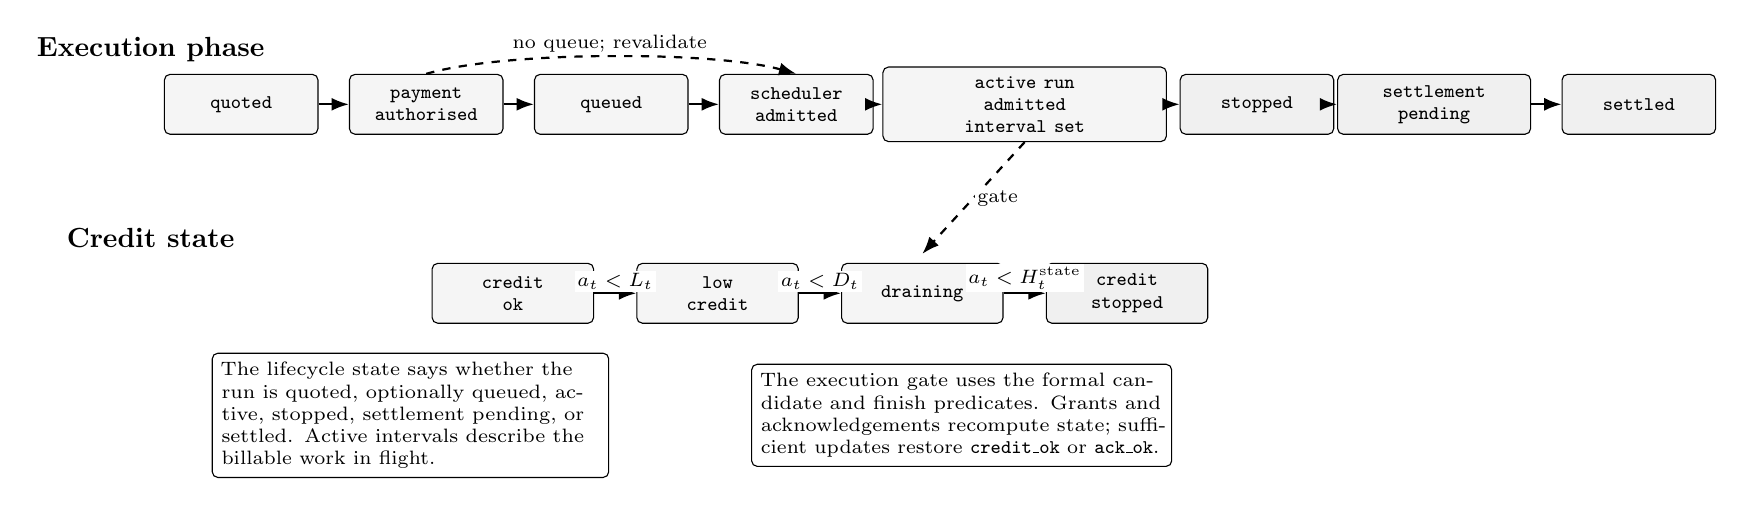
\begin{tikzpicture}[x=1cm,y=1cm, font=\scriptsize]
  \node[font=\bfseries] at (-7.05,1.65) {Execution phase};
  \node[state, minimum width=1.95cm] (quoted) at (-5.9,0.95) {\texttt{quoted}};
  \node[state, minimum width=1.95cm] (auth) at (-3.55,0.95) {\texttt{payment}\\\texttt{authorised}};
  \node[state, minimum width=1.95cm] (queued) at (-1.2,0.95) {\texttt{queued}};
  \node[state, minimum width=1.95cm] (admit) at (1.15,0.95) {\texttt{scheduler}\\\texttt{admitted}};
  \node[state, minimum width=3.6cm, text width=3.25cm] (active) at (4.05,0.95) {\texttt{active run}\\\texttt{admitted}\\\texttt{interval set}};
  \node[state, minimum width=1.95cm, fill=gray!12] (stopExec) at (7.0,0.95) {\texttt{stopped}};
  \node[state, minimum width=2.45cm, fill=gray!12] (pendingSettle) at (9.25,0.95) {\texttt{settlement}\\\texttt{pending}};
  \node[state, minimum width=1.95cm, fill=gray!12] (settled) at (11.85,0.95) {\texttt{settled}};

  \draw[flow] (quoted.east) -- (auth.west);
  \draw[flow] (auth.east) -- (queued.west);
  \draw[flow] (queued.east) -- (admit.west);
  \draw[flow, dashed] (auth.north) .. controls (-2.55,1.63) and (0.1,1.63) .. node[above, fill=white, inner sep=1pt] {no queue; revalidate} (admit.north);
  \draw[flow] (admit.east) -- (active.west);
  \draw[flow] (active.east) -- (stopExec.west);
  \draw[flow] (stopExec.east) -- (pendingSettle.west);
  \draw[flow] (pendingSettle.east) -- (settled.west);

  \node[font=\bfseries] at (-7.05,-0.75) {Credit state};
  \node[state, minimum width=2.05cm] (ok) at (-2.45,-1.45) {\texttt{credit}\\\texttt{ok}};
  \node[state, minimum width=2.05cm] (low) at (0.15,-1.45) {\texttt{low}\\\texttt{credit}};
  \node[state, minimum width=2.05cm] (drain) at (2.75,-1.45) {\texttt{draining}};
  \node[state, minimum width=2.05cm, fill=gray!12] (stopCredit) at (5.35,-1.45) {\texttt{credit}\\\texttt{stopped}};

  \draw[payflow] (ok.east) -- node[above, fill=white, inner sep=1pt] {\(a_t<L_t\)} (low.west);
  \draw[payflow] (low.east) -- node[above, fill=white, inner sep=1pt] {\(a_t<D_t\)} (drain.west);
  \draw[payflow] (drain.east) -- node[above, fill=white, inner sep=1pt] {\(a_t<H_t^{\mathrm{state}}\)} (stopCredit.west);
  \draw[riskflow] (active.south) -- node[right, fill=white, inner sep=1pt] {gate} (2.75,-0.95);

  \node[note, text width=4.8cm] at (-3.75,-3.0)
    {The lifecycle state says whether the run is quoted, optionally queued, active, stopped, settlement pending, or settled. Active intervals describe the billable work in flight.};
  \node[note, text width=5.1cm] at (3.25,-3.0)
    {The execution gate uses the formal candidate and finish predicates. Grants and acknowledgements recompute state; sufficient updates restore \texttt{credit\_ok} or \texttt{ack\_ok}.};
\end{tikzpicture}%
}
\caption{\mppi{} production run lifecycle with credit-state overlay. Here \(a_t\) is available amount, \(L_t\) is the low watermark, \(D_t\) is the money-denominated drain-entry watermark, and \(H_t^{\mathrm{state}}\) is the scalar credit-state projection. Execution phases, monetary credit state, and acknowledgement-lag state are separate axes; implementations admit new billable intervals only when the credit and delivery-lag guards permit it.}
\label{fig:mppi-state-machine}
\end{figure}

Metering boundaries depend on the serving stack and implementation. A provider may define boundaries such as after the next meter frame, after a configured delivered sequence range, after a per-run decode window, after an accepted speculative-token burst, or after a bounded tool, multimodal, KV hold, or scheduler-admitted accelerator interval when that unit has been explicitly quoted. The quote should disclose the policy. The key property is that buyers and facilitators can reason about unpaid admitted work under the selected risk-budget or hard-bound profile when a low-credit, drain-entry, hard-stop, or acknowledgement-lag transition occurs, and that inference stops at the next disclosed boundary when the headroom rule or delivery-lag guard fails.

A non-normative text streaming profile could meter at the smaller of \(N\) delivered tokens, \(T\) milliseconds, or the current per-run decode window. The same profile should define maximum buffered bytes or tokens, maximum acknowledgement-lag range, maximum decode window, maximum tool interval, and profile-handled overshoot after the last valid gate. Under that shape, unpaid admitted work after a missed top-up is hard-bounded by the disclosed cost to the next boundary in a deterministic profile, or risk-budgeted by the selected latency-risk profile, rather than by the full possible output length.

Final receipts should carry a terminal reason such as \field{completed}, \field{client_cancelled}, \field{policy_expired}, \field{credit_exhausted}, \field{provider_failed}, or \field{provider_cancelled}. Cancellation and expiry are effective at the next enforceable metering boundary unless the provider can stop sooner without violating the stream or receipt semantics. A transport profile should define \field{Cancel}, \field{CancelAck}, \field{Stop}, and terminal sequencing, including the cancellation request sequence, engine cancellation attempt, effective cancellation boundary, final billable interval, release-state requirement, and stale cancel or top-up precedence. After policy expiry, the provider must not admit a new billable interval or accept additional grants under that policy; it may only finish an already admitted bounded interval, stop at the next boundary, and settle quoted, metered units. Partial run and failed run pricing must be quoted before execution. Only delivered output included in the signed delivered sequence and acknowledgement boundary defined by the profile is billable as output. Generated but undelivered output is provider risk unless a separately quoted billable event that is not output has already been admitted, metered, and receipted. Units that are not output are billable only when the quote, meter frames, and final receipt make them explicit.

\begin{table}[H]
\centering
\caption{Terminal reasons and billing rule}
\label{tab:terminal-pricing}
\begin{tabularx}{\linewidth}{>{\bfseries\raggedright\arraybackslash}p{0.24\linewidth} >{\raggedright\arraybackslash}X}
\toprule
Terminal reason & Billing rule \\
\midrule
\field{completed} & Settle the final metered amount due subject to the settlement cap: latest valid cumulative grant, client policy maximum, and run claimable limit. \\
\field{client_cancelled} & Bill only previously quoted, already admitted, metered units up to the effective cancellation boundary; bill output only when delivered under the profile's delivery and acknowledgement rule. \\
\field{policy_expired} & Admit no new billable interval after expiry; finish only an already admitted bounded interval, then settle quoted and metered units. \\
\field{credit_exhausted} & Drain through authorised headroom, stop at the disclosed boundary, and settle metered units up to the cap. \\
\field{provider_failed} & Do not bill undelivered output; bill units that are not output only if the quote explicitly made the already admitted unit billable on provider failure. \\
\field{provider_cancelled} & Treat provider-side cancellation as provider risk unless the quote separately priced an already admitted billable event and the meter frames prove it. \\
\bottomrule
\end{tabularx}
\end{table}

\section{MPP Compatibility and Settlement Methods}

\mppi{} should be payment method flexible. The MPP outer flow provides the challenge, credential, and receipt envelope. \mppi{} provides the inference lifecycle inside that envelope. The selected payment method or settlement path defines claimability, settlement mechanics, and finality assumptions.

\subsection{Direct Mode}

In direct mode, the client or inference wallet presents \mppi{} credit grants directly to the provider in a form the provider can verify, backed by the selected MPP payment method. This avoids making a facilitator mandatory. It requires the provider to verify grant signatures, funding or claimability, replay protection, policy limits, and concurrent run claimability.

Direct mode is viable only when each run has a verifiable spend lock, escrow, nonce, channel state, provider allowance, or equivalent atomic claimability that prevents the same funds from backing two concurrent inference runs at once. A free-floating wallet signature that merely states a willingness to pay is not enough for unknown counterparties. Shared funding sources are acceptable, but each inference run needs a distinct reservation or claim path.

In object terms, direct mode should bind \field{InferencePolicy}, \field{CreditGrant}, \field{RunPaymentState}, and \field{FinalReceipt} to a \field{claim_reference_hash} or profile-defined claim-reference commitment/null value. The method profile defines whether that hash commits to escrow state, an allowance nonce, a voucher channel state root, another claimable object the provider can verify cheaply, or a signed method-level convention where no separate claim object exists. A null convention is valid only when the method-level payload still gives the provider verifiable run-scoped claimability. The same method profile should define \field{run_claimable_limit} for that construction.

\subsection{Facilitated Mode}

Facilitated mode introduces a payment coordinator between the wallet and provider. The facilitator can reserve funds per run, issue credit assurances that providers can verify, prevent double spend across concurrent runs, batch settlement, and provide a common wallet integration point. x402 already describes facilitators as optional services that verify payment payloads and settle payments on behalf of servers \cite{x402facilitator}. \mppi{} can use the same adoption logic while adding reservations for inference and cumulative grant semantics.

In this paper, an \mppi{} facilitator is a protocol-level credit-assurance role. It may be implemented by, or layered above, an x402 facilitator, but the base x402 facilitator role is not assumed to provide reservations per run unless the chosen payment method specifies that behaviour.

Facilitated mode can provide run-level isolation when the underlying settlement method does not expose a cheap atomic reservation primitive to every provider. It is a plausible first adoption path for unknown agents and decentralised inference providers, especially where providers want a lower integration burden and wallets want a single place to enforce spend policy. That adoption path should be validated through latency, integration burden, capital efficiency, facilitator economics, and provider adoption measurements. The protocol should still support direct mode to avoid making any one facilitator category mandatory.

In facilitated mode, \field{claim_reference_hash} should commit to the facilitator's run reservation or credit-assurance object. That lets the provider verify that the grant is not only signed for the right run, but also tied to a reservation that the facilitator cannot reuse across concurrent runs.

\subsection{Compatibility Mapping}

\begin{table}[htbp]
\centering
\caption{How existing and proposed payment methods and schemes can support \mppi{}}
\label{tab:compatibility-mapping}
\begin{tabularx}{\linewidth}{>{\raggedright\arraybackslash}p{0.22\linewidth} >{\raggedright\arraybackslash}X}
\toprule
\textbf{Method or scheme} & \textbf{Likely \mppi{} role} \\
\midrule
Proposed MPP \field{inference} intent or private profile identifier & Payment admission envelope for quotes, authorisation scoped to the run, cumulative grants, and final inference receipts. \\
MPP session & Reusable payment state that can carry cumulative vouchers and refreshed credit for inference runs. \\
Charge-style stablecoin methods & Initial funding, explicit top-ups, final settlement, and receipts when amounts are known or bounded. \\
x402 \field{upto} & Adjacent capped-request payment primitive; useful comparison or compatibility context, but not a full inference execution lifecycle by itself. \\
x402 batch settlement & Efficient redemption of many small cumulative grants across runs, when paired with \mppi{} run binding, sequencing, and execution-gate visibility. \\
Facilitator backed credit assurance & Onboarding path for agents, wallets, and decentralised providers. \\
\bottomrule
\end{tabularx}
\end{table}

\section{Security and Abuse Considerations}

\mppi{} moves payment decisions closer to the serving scheduler. That improves economic control but creates a serious security surface. The base threat model should assume malicious clients, malicious providers, malicious or buggy facilitators, collusion between provider and facilitator, compromised delegated signers, network attackers replaying or reordering messages, metadata observers, stale cancel/top-up races, settlement finality or reversal failures, and denial of service attempts against accelerator capacity and serving queues.

\begin{longtable}{>{\raggedright\arraybackslash}p{0.24\linewidth} >{\raggedright\arraybackslash}p{0.25\linewidth} >{\raggedright\arraybackslash}p{0.41\linewidth}}
\caption{Abuse paths and mitigations}\label{tab:abuse-mitigations}\\
\toprule
\textbf{Abuse path} & \textbf{Risk} & \textbf{Mitigation} \\
\midrule
\endfirsthead
\toprule
\textbf{Abuse path} & \textbf{Risk} & \textbf{Mitigation} \\
\midrule
\endhead
Replay of a \field{CreditGrant} & Free or over-authorised inference. & Bind grants to grant ID, grant sequence, \field{run_id}, policy ID, provider ID, request commitment, validity interval, cumulative amount, acknowledged meter frame sequence, and payment method. Require strictly increasing grant sequences. \\
Double spend across concurrent runs & Provider accepts credit that is not actually available. & Use facilitator-enforced run-level reservations or direct mode state that the provider can verify atomically. \\
Provider streams beyond credit & Provider may be unpaid; buyer may later dispute. & Enforce payment synchronisation state in the gateway and scheduler, not just in logs. \\
Malicious provider metering & Buyer is overcharged for delivered output or provider-observed units. & Require tokenizer ID, unit schedule, signed cumulative meter frames, content-private delivered unit commitments, and explicit policy for compute that is not returned as output. Provider-observed units need a declared provider assumption, attestation profile, or dispute-opening profile before independent verifiability is claimed. \\
Buyer underfunds prefill and abandons & Provider pays prefill cost without recovery. & Require initial prefill credit before serving-engine execution. Define cancellation and failed run pricing. \\
Cancel after prefill abuse & Buyer cancels after provider has incurred quoted prefill or tool cost. & Apply cancellation at the next enforceable metering boundary and bill only previously quoted, admitted, metered units. \\
Provider claims generated but undelivered output & Buyer is charged for output it never received. & Bill output only when included in the signed delivered sequence and acknowledged at the profile's application-layer boundary; generated but undelivered output stays provider risk. \\
Low credit race & Stream stalls or runs unpaid beyond policy. & Define low and drain-entry watermarks, grant refresh cadence, required headroom, and drain or stop at a disclosed metering boundary. \\
Stale cancel or top-up race & Old control messages reopen, cancel, or underfund a terminal run. & Sign and sequence \field{DeliveryAck}, \field{Resume}, \field{Cancel}, \field{Stop}, grants, and terminal messages; define race precedence and make terminal settlement idempotent. \\
KV cache hold abuse & Buyer ties up scarce memory cheaply. & If KV hold is offered as a billable unit, make it explicit, priced, capped, metered, receipted, and automatically released on expiry or insufficient credit. \\
Malicious quote changes & Buyer authorises one price and is billed another. & Bind policy to quote ID, provider ID, inference target, tokenizer version, serialisation profile, exact unit prices or price schedule hash, accepted payment method, settlement destination, max context/output, and expiry. \\
Compromised delegated signer & Budget drain. & Use strict delegation: max total, max unit prices, provider allowlist, model allowlist, short expiry, revocation, and wallet visible receipts. \\
Malicious facilitator credit assurance & Provider accepts false credit or buyer funds are over reserved. & Bind facilitator assurances to run, policy, quote, latest accepted meter frame, acknowledgement references where used, reservation amount, and settlement path; expose wallet-visible limits and reservation state that providers can verify. \\
Provider-facilitator collusion & Colluding parties may approve credit against false meter frames, suppress disputes, or misreport provider-observed units. & Binding alone does not independently verify provider-observed units. Profiles that need independent verifiability should require client-side \field{DeliveryAck} verification for output, third-party tool receipts where tools are billed, attestations, audit logs, or dispute-opening profiles. Otherwise the receipt must state the residual provider/facilitator trust assumption. \\
Metadata observation & Payment/control traffic reveals inference target, timing, usage, payer/provider linkage, or settlement linkage. & Keep raw prompt, raw output, and transcript off the payment plane; use content-private commitments, field placement rules, unlinkable run identifiers where feasible, settlement references that are unlinkable where the payment method permits it, and minimal disclosed metadata. \\
Duplicate settlement & Buyer is charged twice after retry or reconnect. & Use cumulative grants, terminal meter frame references, settlement caps, and a stable idempotency key for the final receipt and settlement attempt. \\
Settlement finality failure & A settlement reference is later reversed, reorganised, timed out, or disputed under the selected payment method. & Receipts should report settlement status and finality; profiles must define retry, reversal, timeout, and finality handling per payment method. \\
Receipt omission & Disputes cannot be reconciled. & Provider must emit a final receipt at completion; the client or wallet should store it. If the final receipt is missed after settlement, the settlement reference plus signed cumulative meter frames provide fallback evidence. \\
\bottomrule
\end{longtable}

The most important implementation rule is that payment state must gate execution. If the provider only checks payment after the serving engine has already run, \mppi{} becomes a receipt format, not an execution protocol.

\section{Product Positioning}

\mppi{} should be positioned as an inference-native payment profile, not as a settlement product or generic checkout flow. A clean positioning statement is:

\begin{quote}
\textbf{\mppi{} is a proposed MPP-compatible, inference-native payment profile for metered inference. MPP provides interoperable challenge, credential, and receipt flows. \mppi{} defines the protocol mechanics for candidate interval admission, admitted-interval finishability, drain, stop, settlement, and final inference receipts.}
\end{quote}

\subsection{Agents}

Agents require payable inference across organisational boundaries without a human checkout step or provider-specific onboarding for every call path. The protocol must let them discover inference providers, compare price and latency, authorise bounded spend, receive auditable delivered-unit receipts, and stop at a declared boundary when budget is exhausted.

\subsection{Inference Providers}

Providers need to expose inference endpoints that machines can pay for at admission and during execution. They need to verify authorisation before serving-engine execution, claim payment for prefill and decode under the selected payment method, avoid streaming beyond authorised amount, and handle midstream budget exhaustion without turning payment state into an after-the-fact billing record.

\subsection{Wallets and Facilitators}

Inference wallets and facilitators need a standard way to represent inference spend policies and issue or verify credit grants. They can enforce maximum spend, unit prices, inference-target allowlists, delegated signing rules, run reservations, and receipt collection for autonomous clients and human users without making any wallet implementation part of the core protocol.

\subsection{Where Early Adoption Should Start}

The first adoption hypothesis is facilitated agent-to-provider inference, especially independent providers, inference marketplaces, decentralised provider networks, and APIs that want machine-payable distribution without bespoke commercial setup for every client. This is not a limit on adoption. Any inference provider can adopt \mppi{} where machine payment, bounded spend, cumulative metering, and auditable receipts are useful.

This hypothesis should be validated by integration burden, latency overhead, facilitator economics, capital efficiency, and provider willingness to expose machine-payable inference endpoints.

\section{Reference Implementation and Measurement}

A reference implementation should validate the profile rather than limit it. Text-only inference is a useful first test case because it makes prefill, decode, delivered output, and token metering easy to inspect, but the profile surface should also represent reasoning tokens, tool calls, multimodal units, KV hold time, and scheduler-admitted accelerator time when those units are explicitly quoted, metered, and receipted.

\subsection{Direct and Facilitated Profiles}

A direct profile should let a client or inference wallet submit cumulative credit grants that providers can verify without a mandatory facilitator. A facilitated profile should add a coordinator that reserves funds per run, issues grants that providers can verify, prevents double spend across concurrent runs, and batches settlement when appropriate. Both profiles should use the same \mppi{} quote, policy, meter frame, low-credit, drain, stop, settlement reference, and final receipt semantics.

\subsection{Protocol Coverage}

A reference implementation should cover the six wire objects above plus provider-local \field{RunPaymentState}. It should gate prefill on initial authorisation, gate decode on synchronised payment state, emit low-credit and drain events, stop deterministically at the disclosed boundary, and handle duplicate, lost, delayed, and out-of-order control messages without double counting. It also needs to demonstrate that the payment/control plane never carries raw prompt, raw output, or raw transcript.

\subsection{Measurement}

The implementation should report:

\begin{itemize}
  \item TTFT p50/p95/p99 delta versus a baseline streaming inference call.
  \item ITL p50/p95/p99 delta under expected grant refresh cadence.
  \item Total output TPS, active sequence count, batch size or decode window size, and queue depth.
  \item Credit grant verification latency at p50/p95/p99/p99.9 under high-output-rate streams.
  \item Scheduler visibility lag between accepted grant and serving-path admission decision.
  \item GPU utilisation, GPU memory utilisation, and KV-cache pressure.
  \item Profile-bounded unpaid admitted work, including metering-boundary overshoot and tail handling defined by the profile.
  \item Maximum buyer authorised amount at any point.
  \item Number and size of meter frames and credit grants.
  \item Frequency of low-credit, drain-entry, and hard-stop events.
  \item Reconciliation between final receipt, meter frames, \field{settlement_target_amount}, and \field{settled_amount}.
  \item Cancellation, slow-consumer, and reconnect tests.
  \item Duplicate, lost, delayed, and out-of-order control-message tests.
  \item Maximum unpaid overshoot under induced grant delay, verifier delay, network jitter, and reconnect.
\end{itemize}

\section{Open Questions}

These questions do not change the core thesis; they define the work required to turn the paper-level proposal into interoperable profiles.

\begin{longtable}{>{\raggedright\arraybackslash}p{0.26\linewidth} >{\raggedright\arraybackslash}p{0.64\linewidth}}
\caption{Open specification questions}\label{tab:open-questions}\\
\toprule
\textbf{Question area} & \textbf{Why it matters} \\
\midrule
\endfirsthead
\toprule
\textbf{Question area} & \textbf{Why it matters} \\
\midrule
\endhead
Privacy-preserving commitments & The specification needs an exact hiding commitment construction, canonicalisation rule, and domain separation profile without exposing raw prompt, output, or transcript material. \\
Facilitator economics & Facilitators must reserve capital per run, price credit assurance risk, and remain fast enough for high-output-rate inference. \\
Direct mode reservations & Direct implementations need concrete escrow, nonce, channel, allowance, or atomic claim mechanisms that providers can verify cheaply and bind to one inference run. \\
Settlement finality & Different payment methods have different finality, reversal, timeout, and batch settlement assumptions; \mppi{} receipts need to report those states clearly and profiles need retry and reversal handling for each payment method. \\
Failed run pricing & Table~\ref{tab:terminal-pricing} gives the paper-level rule; formal profiles still need exact pricing rules for partial execution, provider failure, client cancellation, tool failure, and policy expiry. \\
Dispute evidence & The base profile can preserve evidence, but later profiles must decide when and how commitments, meter frames, or private records are opened during disputes, and who is authorised to open them. \\
Provider-observed units and attestation & Reasoning tokens, internal compute, tool units, KV hold time, and scheduler-admitted accelerator time need explicit quote, meter, provider assumptions, and attestation or dispute-opening rules before profiles claim independent verifiability. \\
Transport profiles & SSE plus side-channel POST, WebSocket, HTTP/2/gRPC, and HTTP/3/WebTransport need common ordering, replay, reconnect, flow-control, backpressure, acknowledgement cadence, cancellation, half-close, and terminal message requirements. \\
Provider integration burden & Gateways, schedulers, wallets, and facilitators need reference measurements showing whether \mppi{} can protect TTFT and ITL while bounding unpaid admitted work under a disclosed profile. \\
\bottomrule
\end{longtable}

\section{Specification Direction}

The paper makes a small set of clear decisions. A formal specification should turn these decisions and the open questions above into canonical object schemas, protocol versioning, serialisation rules, object type tags, signature suites, domain separation, privacy profiles, transport profiles, settlement method mappings, dispute opening rules, error codes, and reference implementation measurements.

\begin{enumerate}
  \item \mppi{} should be specified as an MPP payment profile for inference, with \field{inference} as the proposed payment intent name and the inference execution lifecycle rules defined by the \mppi{} profile. Until \field{inference} is registered or otherwise accepted by the relevant MPP or Payment HTTP process, experimental deployments should identify it as a private or provisional \mppi{} profile identifier, or carry it under a registered intent through a profile-specific adapter.
  \item MPP should provide the outer \field{402} challenge, credential, and receipt envelope. \mppi{} should define the inference execution lifecycle inside that envelope.
  \item The profile should define two logical planes: an inference plane for private request and delivered output, and a payment/control plane for policies, grants, meter frames, low-credit events, settlement references, and receipts.
  \item HTTP/2 or gRPC independent streams are a good high-performance profile. SSE plus side-channel POST, WebSocket, and HTTP/3/WebTransport should also be compatible when they preserve ordering, replay protection, run binding, delivery acknowledgement, and privacy boundaries.
  \item Transport profiles should define signed and sequenced \field{DeliveryAck}, \field{Resume}, \field{Cancel}, \field{Stop}, and terminal messages, including state vectors and race precedence.
  \item The profile should define \field{run_id} creation before policy signing, including the exact dependency order for provider-created and nonce-derived identities. \field{InferenceQuote} should carry either a provider-created \field{run_id} or provider run nonce; the policy body should include the resulting run identity before \field{policy_hash} is computed; and \field{InferencePolicy}, the genesis \field{CreditGrant}, \field{DeliveryAck}, \field{MeterFrame}, and \field{FinalReceipt} should bind the same run identity.
  \item Signed fields in \field{DeliveryAck}, \field{CreditGrant}, \field{MeterFrame}, and \field{FinalReceipt} should bind \field{run_id}, policy ID, quote ID where relevant, provider ID, \field{claim_reference_hash} or profile-defined claim-reference commitment/null value, sequence numbers, payment-state version where relevant, acknowledged meter frame sequence, acknowledged delivered sequence or range where output billing uses acknowledged delivery, cumulative authorised amount, \field{cumulative_amount_due}, usage totals, timing policy, settlement reference, receipt transport or reference method, and content-private commitments.
  \item Reconnects, duplicate messages, delayed messages, and out-of-order messages should be handled through cumulative grants, cumulative meter frames, strictly increasing sequences, and idempotent settlement against the latest valid cumulative state.
  \item Credit-grant profiles should define causal grant acceptance under meter-frame concurrency: non-decreasing grant sequence, cumulative authorised amount, acknowledged meter-frame sequence, replay-window or acceptance-window bounds, terminal-state rejection, and reconnect behaviour.
  \item Grant validity, policy expiry, and settlement-method claimability should state their decision points explicitly: candidate admission, interval finish, meter posting, settlement submission, finality, or a profile-defined claimability snapshot for active admitted intervals.
  \item Prefill should be priced before serving-engine execution through exact tokenisation where possible, or through a conservative bound that is corrected before execution begins. The quote should bind tokenizer version, serialisation profile, special-token policy, tool schema hash, multimodal preprocessing profile, context-window policy, and cache-hit class where relevant.
  \item Headroom and top-up rules should be denominated in the selected payment method's smallest unit, using the payment synchronisation invariant plus a disclosed risk-budget or hard-bound profile that covers grant RTT, verification, scheduler visibility, retry, reconnect, and every active billable unit type that can accrue before the execution gate sees the control decision. The execution gate should also enforce a separate acknowledgement-lag state for delivered but unacknowledged output as flow-control/provider-risk exposure, not as settled billable output under the base profile.
  \item Profiles should define per-run admitted intervals rather than relying on a global scheduler batch as the billing boundary. Valid intervals may include prefill admission, chunked-prefill segment, per-run decode window, accepted speculative-token burst, tool interval, multimodal interval, KV hold lease, or scheduler-admitted accelerator interval. Each interval should bind a quote line item, metering-boundary profile, unit bound, price schedule, rounding rule, and computed maximum cost \(C_j^{\max}\).
  \item Output billing should apply only to acknowledged delivered output covered by delivery and acknowledgement semantics defined by the profile plus signed metering commitments. Generated but undelivered output remains provider risk.
  \item Accepted speculative tokens may be billed as delivered output once delivered under the profile. Rejected draft work should remain provider risk unless explicitly priced under an attestation, audit, or dispute-opening profile.
  \item Units that are not output, such as cached input, reasoning tokens, tool calls, multimodal units, KV hold time, and scheduler-admitted accelerator time, should be billable only when explicitly quoted, metered, receipted, and covered by a declared provider assumption, attestation profile, or dispute-opening profile where independent verifiability is claimed. Non-output billable-event records should carry billable unit type, admitted interval, pricing reference, evidence profile, evidence hash or root, and any third-party receipt, provider assertion, audit, attestation, or dispute-opening reference used by that profile.
  \item Cached-input quotes should distinguish committed cache hits, best-effort cache hits, and fallback misses. If a best-effort hit becomes an uncached prefill, the profile should require a corrected quote or fresh grant before the expensive prefill interval begins.
  \item \begin{minipage}[t]{\linewidth}\raggedright Final receipts should include canonical usage and cap fields: \field{usage_totals}, \field{final_metered_amount_due}, \field{settlement_cap}, and \field{run_claimable_limit}. They should also include the canonical settlement and refund fields in Table~\ref{tab:canonical-settlement-fields}, \field{settlement_cap_cause}, \field{authorisation_shortfall_reason} where applicable, \field{claim_reference_hash} or claim-reference binding, \field{unused_authorisation_amount}, \field{released_run_claimable_amount} or reservation release state, \field{settlement_reference}, \field{settlement_status}, \field{settlement_finality}, terminal \field{DeliveryAck} where used, content-private delivered unit commitments, billable event evidence commitments, and non-output evidence roots by default, not raw output or transcript material.\end{minipage}
\end{enumerate}

\section{Conclusion}

Machine payment protocols can already move value around HTTP resources. That matters for inference, but it does not solve the execution-control problem by itself. Metered inference needs payment semantics for a stateful, uncertain-cost compute exchange. The provider spends before the first token. The buyer does not know the final output length. Midstream payment failure has real operational cost.

\mppi{} fills the missing layer by defining the inference execution and payment lifecycle inside an MPP payment envelope. Its core primitive is synchronised payment state: a new billable inference interval may be admitted only while \(a_t\) covers the candidate admission headroom \(H_{j,t}^{\mathrm{admit}(q)}\), the candidate drain-entry threshold \(D_{j,t}\), the acknowledgement-lag guard, and the finishability of all intervals that would be active after admission. An already admitted bounded interval may finish only while its interval-specific finish headroom remains covered at the next enforceable metering boundary. Around that primitive, \mppi{} defines quotes, policies, cumulative credit grants, signed meter frames, explicit low-credit and drain states, stop behaviour, settlement references, and final receipts.

This is a pragmatic trade-off. \mppi{} does not prove output quality or mandate a settlement method. It makes the payment state of an inference run explicit enough that agents and users can spend under bounded policy, providers can serve machine clients with hard-bounded exposure under deterministic profiles or risk-budgeted exposure under disclosed quantile profiles, and wallets or facilitators can enforce budgets without putting payment in the path of every token.

A focused next step is a facilitated text inference reference profile with published measurements: TTFT overhead, ITL overhead, grant verification latency, profile-bounded unpaid admitted work, maximum buyer authorisation, reconnect behaviour, and final receipt reconciliation. That profile would give builders a concrete first target while preserving the larger \mppi{} thesis: MPP at admission, built for inference during execution.

\begin{thebibliography}{99}

\bibitem{paymentauth}
Ryan, B., Moxey, J., Meagher, T., Weinstein, J., and Kaliski, S.
\textit{The ``Payment'' HTTP Authentication Scheme}.
Internet-Draft draft-httpauth-payment-00, published June 25, 2026. Accessed June 28, 2026.
\url{https://paymentauth.org/draft-httpauth-payment-00.html}

\bibitem{chargeintent}
Moxey, J., Ryan, B., and Meagher, T.
\textit{``charge'' Intent for HTTP Payment Authentication}.
Internet-Draft draft-payment-intent-charge-00, published June 25, 2026. Accessed June 28, 2026.
\url{https://paymentauth.org/draft-payment-intent-charge-00.html}

\bibitem{evmcharge}
DiNovi, B., Swenberg, C., and Scott, K.
\textit{EVM Charge Intent for HTTP Payment Authentication}.
Internet-Draft draft-evm-charge-00, published June 25, 2026. Accessed June 28, 2026.
\url{https://paymentauth.org/draft-evm-charge-00.html}

\bibitem{solanacharge}
Galabru, L., and Gitter, I.
\textit{Solana Charge Intent for HTTP Payment Authentication}.
Internet-Draft draft-solana-charge-00, published June 25, 2026. Accessed June 28, 2026.
\url{https://paymentauth.org/draft-solana-charge-00.html}

\bibitem{mppsession}
Machine Payments Protocol.
\textit{An improved sessions experience}.
June 17, 2026. Accessed June 28, 2026.
\url{https://mpp.dev/blog/sessions-improved}

\bibitem{mpp}
Machine Payments Protocol.
\textit{MPP: Machine Payments Protocol}.
Accessed June 28, 2026.
\url{https://mpp.dev/}

\bibitem{x402exact}
x402.
\textit{Exact: Fixed price x402 payments}.
Accessed June 28, 2026.
\url{https://docs.x402.org/schemes/exact}

\bibitem{x402upto}
x402.
\textit{Upto: Usage-based x402 payments}.
Accessed June 28, 2026.
\url{https://docs.x402.org/schemes/upto}

\bibitem{x402batch}
x402.
\textit{Batch Settlement: High throughput EVM payments}.
Accessed June 28, 2026.
\url{https://docs.x402.org/schemes/batch-settlement}

\bibitem{x402facilitator}
x402.
\textit{Facilitator}.
Accessed June 28, 2026.
\url{https://docs.x402.org/core-concepts/facilitator}

\bibitem{nvidiaMetrics}
NVIDIA.
\textit{NVIDIA NIM LLMs Benchmarking: Metrics}.
Last updated April 1, 2026. Accessed June 28, 2026.
\url{https://docs.nvidia.com/nim/benchmarking/llm/latest/metrics.html}

\bibitem{pagedAttention}
Kwon, W., Li, Z., Zhuang, S., Sheng, Y., Zheng, L., Yu, C. H., Gonzalez, J. E., Zhang, H., and Stoica, I.
\textit{Efficient Memory Management for Large Language Model Serving with PagedAttention}.
SOSP 2023. Accessed June 28, 2026.
\url{https://arxiv.org/abs/2309.06180}

\bibitem{vllmBlog}
Kwon, W., Li, Z., Zhuang, S., Sheng, Y., Zheng, L., Yu, C., Gonzalez, J., Zhang, H., and Stoica, I.
\textit{vLLM: Easy, Fast, and Cheap LLM Serving with PagedAttention}.
June 2023. Accessed June 28, 2026.
\url{https://vllm.ai/blog/2023-06-20-vllm}

\bibitem{bedrockQuota}
Amazon Web Services.
\textit{How tokens are counted in Amazon Bedrock}.
Accessed June 28, 2026.
\url{https://docs.aws.amazon.com/bedrock/latest/userguide/quotas-token-burndown.html}

\bibitem{ap2}
Parikh, S., and Surapaneni, R.
\textit{Powering AI commerce with the new Agent Payments Protocol (AP2)}.
Google Cloud Blog, September 16, 2025. Accessed June 28, 2026.
\url{https://cloud.google.com/blog/products/ai-machine-learning/announcing-agents-to-payments-ap2-protocol}

\bibitem{a2ax402}
Google Agentic Commerce.
\textit{A2A x402 Extension}.
GitHub repository, v0.1.0 released September 16, 2025. Accessed June 28, 2026.
\url{https://github.com/google-agentic-commerce/a2a-x402}

\bibitem{polygonInferenceBilling}
Polygon.
\textit{Per-inference billing for AI APIs}.
Polygon Developer Docs. Accessed June 28, 2026.
\url{https://docs.polygon.technology/payment-services/agentic-payments/solutions/per-inference-billing}

\bibitem{fortytwoEscrow}
Fortytwo Network.
\textit{x402Escrow}.
GitHub repository. Accessed June 28, 2026.
\url{https://github.com/Fortytwo-Network/fortytwo-x402Escrow}

\bibitem{x402LogicFlaws}
Ling, S., Huang, Y., Du, Y., Chen, Y., Zhou, Y., Wu, L., and Wang, C.
\textit{Free-Riding the Agentic Web: A Systematic Security Analysis of x402 Payments}.
arXiv:2605.30998, submitted May 29, 2026; revised June 22, 2026. Accessed June 28, 2026.
\url{https://arxiv.org/abs/2605.30998}

\end{thebibliography}

\end{document}
